\documentclass[]{book}
\usepackage{lmodern}
\usepackage{amssymb,amsmath}
\usepackage{ifxetex,ifluatex}
\usepackage{fixltx2e} % provides \textsubscript
\ifnum 0\ifxetex 1\fi\ifluatex 1\fi=0 % if pdftex
  \usepackage[T1]{fontenc}
  \usepackage[utf8]{inputenc}
\else % if luatex or xelatex
  \ifxetex
    \usepackage{mathspec}
  \else
    \usepackage{fontspec}
  \fi
  \defaultfontfeatures{Ligatures=TeX,Scale=MatchLowercase}
\fi
% use upquote if available, for straight quotes in verbatim environments
\IfFileExists{upquote.sty}{\usepackage{upquote}}{}
% use microtype if available
\IfFileExists{microtype.sty}{%
\usepackage[]{microtype}
\UseMicrotypeSet[protrusion]{basicmath} % disable protrusion for tt fonts
}{}
\PassOptionsToPackage{hyphens}{url} % url is loaded by hyperref
\usepackage[unicode=true]{hyperref}
\hypersetup{
            pdftitle={Essential R Skills},
            pdfauthor={UMN-Morris Statistics Discipline},
            pdfborder={0 0 0},
            breaklinks=true}
\urlstyle{same}  % don't use monospace font for urls
\usepackage{natbib}
\bibliographystyle{apalike}
\usepackage{color}
\usepackage{fancyvrb}
\newcommand{\VerbBar}{|}
\newcommand{\VERB}{\Verb[commandchars=\\\{\}]}
\DefineVerbatimEnvironment{Highlighting}{Verbatim}{commandchars=\\\{\}}
% Add ',fontsize=\small' for more characters per line
\usepackage{framed}
\definecolor{shadecolor}{RGB}{248,248,248}
\newenvironment{Shaded}{\begin{snugshade}}{\end{snugshade}}
\newcommand{\KeywordTok}[1]{\textcolor[rgb]{0.13,0.29,0.53}{\textbf{#1}}}
\newcommand{\DataTypeTok}[1]{\textcolor[rgb]{0.13,0.29,0.53}{#1}}
\newcommand{\DecValTok}[1]{\textcolor[rgb]{0.00,0.00,0.81}{#1}}
\newcommand{\BaseNTok}[1]{\textcolor[rgb]{0.00,0.00,0.81}{#1}}
\newcommand{\FloatTok}[1]{\textcolor[rgb]{0.00,0.00,0.81}{#1}}
\newcommand{\ConstantTok}[1]{\textcolor[rgb]{0.00,0.00,0.00}{#1}}
\newcommand{\CharTok}[1]{\textcolor[rgb]{0.31,0.60,0.02}{#1}}
\newcommand{\SpecialCharTok}[1]{\textcolor[rgb]{0.00,0.00,0.00}{#1}}
\newcommand{\StringTok}[1]{\textcolor[rgb]{0.31,0.60,0.02}{#1}}
\newcommand{\VerbatimStringTok}[1]{\textcolor[rgb]{0.31,0.60,0.02}{#1}}
\newcommand{\SpecialStringTok}[1]{\textcolor[rgb]{0.31,0.60,0.02}{#1}}
\newcommand{\ImportTok}[1]{#1}
\newcommand{\CommentTok}[1]{\textcolor[rgb]{0.56,0.35,0.01}{\textit{#1}}}
\newcommand{\DocumentationTok}[1]{\textcolor[rgb]{0.56,0.35,0.01}{\textbf{\textit{#1}}}}
\newcommand{\AnnotationTok}[1]{\textcolor[rgb]{0.56,0.35,0.01}{\textbf{\textit{#1}}}}
\newcommand{\CommentVarTok}[1]{\textcolor[rgb]{0.56,0.35,0.01}{\textbf{\textit{#1}}}}
\newcommand{\OtherTok}[1]{\textcolor[rgb]{0.56,0.35,0.01}{#1}}
\newcommand{\FunctionTok}[1]{\textcolor[rgb]{0.00,0.00,0.00}{#1}}
\newcommand{\VariableTok}[1]{\textcolor[rgb]{0.00,0.00,0.00}{#1}}
\newcommand{\ControlFlowTok}[1]{\textcolor[rgb]{0.13,0.29,0.53}{\textbf{#1}}}
\newcommand{\OperatorTok}[1]{\textcolor[rgb]{0.81,0.36,0.00}{\textbf{#1}}}
\newcommand{\BuiltInTok}[1]{#1}
\newcommand{\ExtensionTok}[1]{#1}
\newcommand{\PreprocessorTok}[1]{\textcolor[rgb]{0.56,0.35,0.01}{\textit{#1}}}
\newcommand{\AttributeTok}[1]{\textcolor[rgb]{0.77,0.63,0.00}{#1}}
\newcommand{\RegionMarkerTok}[1]{#1}
\newcommand{\InformationTok}[1]{\textcolor[rgb]{0.56,0.35,0.01}{\textbf{\textit{#1}}}}
\newcommand{\WarningTok}[1]{\textcolor[rgb]{0.56,0.35,0.01}{\textbf{\textit{#1}}}}
\newcommand{\AlertTok}[1]{\textcolor[rgb]{0.94,0.16,0.16}{#1}}
\newcommand{\ErrorTok}[1]{\textcolor[rgb]{0.64,0.00,0.00}{\textbf{#1}}}
\newcommand{\NormalTok}[1]{#1}
\usepackage{longtable,booktabs}
% Fix footnotes in tables (requires footnote package)
\IfFileExists{footnote.sty}{\usepackage{footnote}\makesavenoteenv{long table}}{}
\usepackage{graphicx,grffile}
\makeatletter
\def\maxwidth{\ifdim\Gin@nat@width>\linewidth\linewidth\else\Gin@nat@width\fi}
\def\maxheight{\ifdim\Gin@nat@height>\textheight\textheight\else\Gin@nat@height\fi}
\makeatother
% Scale images if necessary, so that they will not overflow the page
% margins by default, and it is still possible to overwrite the defaults
% using explicit options in \includegraphics[width, height, ...]{}
\setkeys{Gin}{width=\maxwidth,height=\maxheight,keepaspectratio}
\IfFileExists{parskip.sty}{%
\usepackage{parskip}
}{% else
\setlength{\parindent}{0pt}
\setlength{\parskip}{6pt plus 2pt minus 1pt}
}
\setlength{\emergencystretch}{3em}  % prevent overfull lines
\providecommand{\tightlist}{%
  \setlength{\itemsep}{0pt}\setlength{\parskip}{0pt}}
\setcounter{secnumdepth}{5}
% Redefines (sub)paragraphs to behave more like sections
\ifx\paragraph\undefined\else
\let\oldparagraph\paragraph
\renewcommand{\paragraph}[1]{\oldparagraph{#1}\mbox{}}
\fi
\ifx\subparagraph\undefined\else
\let\oldsubparagraph\subparagraph
\renewcommand{\subparagraph}[1]{\oldsubparagraph{#1}\mbox{}}
\fi

% set default figure placement to htbp
\makeatletter
\def\fps@figure{htbp}
\makeatother

\usepackage{booktabs}
\usepackage{amsthm}
\makeatletter
\def\thm@space@setup{%
  \thm@preskip=8pt plus 2pt minus 4pt
  \thm@postskip=\thm@preskip
}
\makeatother

\title{Essential R Skills}
\author{UMN-Morris Statistics Discipline}
\date{2020-06-02}

\begin{document}
\maketitle

{
\setcounter{tocdepth}{1}
\tableofcontents
}
\chapter{Motivation}\label{motivation}

We have found that students enter our courses with wide variation in
experience and comfort using statistical software for computation and
making graphical displays. This document represents our expectations for
the basic R skills that students should know upon completing an
introductory course in statistics. Analysis methods may appear at times
in this document, but the emphasis here is upon basic R usage for data
wrangling, and exploratory data analysis using numeric and graphical
methods.

\chapter{Getting Started}\label{GettingStarted}

\section{Packages}\label{packages}

When you start R studio, basic functionality is initially available.
However, in most projects we will want to use some special code and
functions contained in packages that are not initially available whe R
starts. Before packages can be used in our analyses, they must be
installed in our R workspace. We presume that the R Studio development
environment is being used by our students. Any package can be installed
by clicking the ``Packages'' tab in the lower right panel of the R
Studio workspace. Then click ``Install'' to produce an entry bar where
you type the name of the desired package.

Once a package is installed into your R Studio environment, you make it
available by loading with the \texttt{library()} command. For this
document, some additional packages are needed, and are loaded in the
next code block. The \emph{knitr} and \emph{tidyverse} packages have
been previously installed. If you attempt to load a package (in this
case zelig) that has not been installed, you will get an error message
similar to this:

\texttt{Error\ in\ library(zelig)\ :\ there\ is\ no\ package\ called\ ‘zelig’}

\begin{Shaded}
\begin{Highlighting}[]
\CommentTok{# this block loads R packages that may be needed for the analysis.}
\KeywordTok{library}\NormalTok{(knitr)}
\KeywordTok{library}\NormalTok{(tidyverse)}
\end{Highlighting}
\end{Shaded}

\section{The tidyverse Package}\label{the-tidyverse-package}

The tidyverse package is very special - it is a package of other
packages. The tidyverse website \href{http://tidyverse.org}{tidyverse}
describes the tidyverse as: \emph{The tidyverse is an opinionated
collection of R packages designed for data science. All packages share
an underlying design philosophy, grammar, and data structures.}

The most important packages inside the tidyverse package for this
document are: dplyr, magrittr, and ggplot.

\section{Gapminder Data:}\label{gapminder-data}

This dataset (named gapminder) is contained in an R package called
\emph{gapminder}, and needs to be loaded before the dataset can be used.

\begin{Shaded}
\begin{Highlighting}[]
\KeywordTok{library}\NormalTok{(gapminder)}
\end{Highlighting}
\end{Shaded}

\section{Set Working Directory}\label{set-working-directory}

In the ``Files'' tab in the lower right portion of the R Studio work
area, you can choose where you want to store files and conduct your work
by navigating to a suitable folder by making folders and sub-folders and
then clicking to navigate to a suitable work area.

You should notify R Studio and the R software to this location called
the working directory. Once you have navigated to where you want files,
data, and results to reside, you notify R Studio by clicking the blue
``More'' gear and choose ``set working directory.'' This will help R
understand where to expect files and dat to be located.

One of the most common problems students experience is that they work on
files in a location not specified as the ``working directory.''

\section{Reading Data From a CSV
File}\label{reading-data-from-a-csv-file}

The most common way to read data into R is from an excel spreadsheet
that has been saved into a comma-separated-values (csv) file. This means
that data elements are separated from each other by commas ``,''.

We consider a data file named (file.csv) that contains variable names in
the first row of the file. Place this file in your working directory and
read,

\begin{Shaded}
\begin{Highlighting}[]
\NormalTok{dataframe <-}\StringTok{ }\KeywordTok{read.csv}\NormalTok{(}\StringTok{"file.csv"}\NormalTok{,}\DataTypeTok{header=}\OtherTok{TRUE}\NormalTok{)}
\end{Highlighting}
\end{Shaded}

The \emph{readr} package inside the \emph{tidyverse} family of packages
has a slightly nicer read csv function you should know about. We use the
\texttt{readr::} prefix to inform readers that the \texttt{read\_csv}
function resides in the \emph{readr} package.

\begin{Shaded}
\begin{Highlighting}[]
\NormalTok{dataframe <-}\StringTok{ }\NormalTok{readr}\OperatorTok{::}\KeywordTok{read_csv}\NormalTok{(}\StringTok{"file.csv"}\NormalTok{,}\DataTypeTok{col_names =} \OtherTok{TRUE}\NormalTok{)}
\end{Highlighting}
\end{Shaded}

Reading data directly from excel spreadsheets is more complex and you
should read documentation for the \emph{readxl} package.

\chapter{Overview of a Dataframe}\label{OverviewDataframe}

Datasets in R are usually called dataframes or tibbles. The distinction
between these names is not important for our purposes - we will usually
refer to a dataset as a dataframe.

\section{glimpse}\label{glimpse}

Let's look at what is inside the gapminder dataset using the
\texttt{glimpse} command from the \emph{dplyr} package. The \emph{dplyr}
package is contained in the package ``tidyverse'' that was loaded
previously. The \texttt{glimpse(gapminder)} command would have executed
without any errors. We use the \texttt{dplyr::} prefix to inform readers
that the glimpse function resides in the \emph{dplyr} package.

\begin{Shaded}
\begin{Highlighting}[]
\CommentTok{# the next command would also execute if}
\CommentTok{# dplyr or tidyverse was loaded..}
\CommentTok{#glimpse(gapminder)}
\NormalTok{dplyr}\OperatorTok{::}\KeywordTok{glimpse}\NormalTok{(gapminder)}
\end{Highlighting}
\end{Shaded}

\begin{verbatim}
## Observations: 1,704
## Variables: 6
## $ country   <fct> Afghanistan, Afghanistan, Afghanistan, Afghanistan, Afghani…
## $ continent <fct> Asia, Asia, Asia, Asia, Asia, Asia, Asia, Asia, Asia, Asia,…
## $ year      <int> 1952, 1957, 1962, 1967, 1972, 1977, 1982, 1987, 1992, 1997,…
## $ lifeExp   <dbl> 28.801, 30.332, 31.997, 34.020, 36.088, 38.438, 39.854, 40.…
## $ pop       <int> 8425333, 9240934, 10267083, 11537966, 13079460, 14880372, 1…
## $ gdpPercap <dbl> 779.4453, 820.8530, 853.1007, 836.1971, 739.9811, 786.1134,…
\end{verbatim}

This shows it contains economic and demographic information about
different countries across years. There are 1704 rows (observations) and
6 columns (variables).

Each variable name is listed along with a variable type designation.

\begin{itemize}
\tightlist
\item
  fct: means a factor variable, also known as a categorical variable.
\item
  int: means a quantitative variable that takes only integer or whole
  number values.
\item
  dbl: means double precision, a quantitative variable that is
  essentially continuous - taking decimal values.
\end{itemize}

\section{head}\label{head}

By default, the \texttt{head} command will show the first 6 rows of the
dataset gapminder. Datasets in R are called ``dataframes.'' The
gapminder dataframe is denoted as a ``tibble'' which is a type of
dataframe.

Options to the head command can change the rows displayed.

\begin{Shaded}
\begin{Highlighting}[]
\CommentTok{# default is to show 6 rows}
\KeywordTok{head}\NormalTok{(gapminder)}
\end{Highlighting}
\end{Shaded}

\begin{verbatim}
## # A tibble: 6 x 6
##   country     continent  year lifeExp      pop gdpPercap
##   <fct>       <fct>     <int>   <dbl>    <int>     <dbl>
## 1 Afghanistan Asia       1952    28.8  8425333      779.
## 2 Afghanistan Asia       1957    30.3  9240934      821.
## 3 Afghanistan Asia       1962    32.0 10267083      853.
## 4 Afghanistan Asia       1967    34.0 11537966      836.
## 5 Afghanistan Asia       1972    36.1 13079460      740.
## 6 Afghanistan Asia       1977    38.4 14880372      786.
\end{verbatim}

\begin{Shaded}
\begin{Highlighting}[]
\CommentTok{# show only 4 rows...}
\KeywordTok{head}\NormalTok{(gapminder,}\DataTypeTok{n=}\DecValTok{4}\NormalTok{)}
\end{Highlighting}
\end{Shaded}

\begin{verbatim}
## # A tibble: 4 x 6
##   country     continent  year lifeExp      pop gdpPercap
##   <fct>       <fct>     <int>   <dbl>    <int>     <dbl>
## 1 Afghanistan Asia       1952    28.8  8425333      779.
## 2 Afghanistan Asia       1957    30.3  9240934      821.
## 3 Afghanistan Asia       1962    32.0 10267083      853.
## 4 Afghanistan Asia       1967    34.0 11537966      836.
\end{verbatim}

\section{summary}\label{summary}

This command shows a basic summary of the values in each variable.

\begin{Shaded}
\begin{Highlighting}[]
\CommentTok{# A basic, base R command}
\KeywordTok{summary}\NormalTok{(gapminder)}
\end{Highlighting}
\end{Shaded}

\begin{verbatim}
##         country        continent        year         lifeExp     
##  Afghanistan:  12   Africa  :624   Min.   :1952   Min.   :23.60  
##  Albania    :  12   Americas:300   1st Qu.:1966   1st Qu.:48.20  
##  Algeria    :  12   Asia    :396   Median :1980   Median :60.71  
##  Angola     :  12   Europe  :360   Mean   :1980   Mean   :59.47  
##  Argentina  :  12   Oceania : 24   3rd Qu.:1993   3rd Qu.:70.85  
##  Australia  :  12                  Max.   :2007   Max.   :82.60  
##  (Other)    :1632                                                
##       pop              gdpPercap       
##  Min.   :6.001e+04   Min.   :   241.2  
##  1st Qu.:2.794e+06   1st Qu.:  1202.1  
##  Median :7.024e+06   Median :  3531.8  
##  Mean   :2.960e+07   Mean   :  7215.3  
##  3rd Qu.:1.959e+07   3rd Qu.:  9325.5  
##  Max.   :1.319e+09   Max.   :113523.1  
## 
\end{verbatim}

The next command illustrates a ``pipe'' - here the dataframe gapminder
is ``piped'' into the summary function to be processed. Note the same
output is produce as using \texttt{summary(gapminder)}. Note, the pipe
operation \%\textgreater{}\% is contained in tidyverse package:
\emph{magrittr} which is loaded when \emph{tidyverse} is loaded.

\begin{Shaded}
\begin{Highlighting}[]
\CommentTok{# Same idea, but using tidyverse pipe}
\NormalTok{gapminder }\OperatorTok\StringTok{ }\KeywordTok{summary}\NormalTok{()}
\end{Highlighting}
\end{Shaded}

\begin{verbatim}
##         country        continent        year         lifeExp     
##  Afghanistan:  12   Africa  :624   Min.   :1952   Min.   :23.60  
##  Albania    :  12   Americas:300   1st Qu.:1966   1st Qu.:48.20  
##  Algeria    :  12   Asia    :396   Median :1980   Median :60.71  
##  Angola     :  12   Europe  :360   Mean   :1980   Mean   :59.47  
##  Argentina  :  12   Oceania : 24   3rd Qu.:1993   3rd Qu.:70.85  
##  Australia  :  12                  Max.   :2007   Max.   :82.60  
##  (Other)    :1632                                                
##       pop              gdpPercap       
##  Min.   :6.001e+04   Min.   :   241.2  
##  1st Qu.:2.794e+06   1st Qu.:  1202.1  
##  Median :7.024e+06   Median :  3531.8  
##  Mean   :2.960e+07   Mean   :  7215.3  
##  3rd Qu.:1.959e+07   3rd Qu.:  9325.5  
##  Max.   :1.319e+09   Max.   :113523.1  
## 
\end{verbatim}

\section{Dataframe Details: funModeling
package}\label{dataframe-details-funmodeling-package}

The \emph{funModeling} package contains the \texttt{df\_status} command
which also summarizes a dataframe - showing different aspects like
missing values, percentage of zero values, and also the number of unique
values.

\begin{Shaded}
\begin{Highlighting}[]
\NormalTok{funModeling}\OperatorTok{::}\KeywordTok{df_status}\NormalTok{(gapminder)}
\end{Highlighting}
\end{Shaded}

\begin{verbatim}
##    variable q_zeros p_zeros q_na p_na q_inf p_inf    type unique
## 1   country       0       0    0    0     0     0  factor    142
## 2 continent       0       0    0    0     0     0  factor      5
## 3      year       0       0    0    0     0     0 integer     12
## 4   lifeExp       0       0    0    0     0     0 numeric   1626
## 5       pop       0       0    0    0     0     0 integer   1704
## 6 gdpPercap       0       0    0    0     0     0 numeric   1704
\end{verbatim}

\begin{Shaded}
\begin{Highlighting}[]
\NormalTok{di=funModeling}\OperatorTok{::}\KeywordTok{data_integrity}\NormalTok{(gapminder)}
\CommentTok{# returns a detailed summary of all variables}
\KeywordTok{print}\NormalTok{(di)}
\end{Highlighting}
\end{Shaded}

\begin{verbatim}
## $vars_num_with_NA
## [1] variable q_na     p_na    
## <0 rows> (or 0-length row.names)
## 
## $vars_cat_with_NA
## [1] variable q_na     p_na    
## <0 rows> (or 0-length row.names)
## 
## $vars_cat_high_card
##   variable unique
## 1  country    142
## 
## $MAX_UNIQUE
## [1] 35
## 
## $vars_one_value
## character(0)
## 
## $vars_cat
## [1] "country"   "continent"
## 
## $vars_num
## [1] "year"      "lifeExp"   "pop"       "gdpPercap"
## 
## $vars_char
## character(0)
## 
## $vars_factor
## [1] "country"   "continent"
## 
## $vars_other
## character(0)
\end{verbatim}

\section{Dataframe Details: skimr
package}\label{dataframe-details-skimr-package}

The \emph{skimr} package contains many useful functions for summarizing
a dataframe. When we supply a dataframe to the
\texttt{skim\_without\_charts} function, dataframe details are separated
by variable types.

\begin{Shaded}
\begin{Highlighting}[]
\NormalTok{gapminder }\OperatorTok\StringTok{ }
\StringTok{  }\NormalTok{skimr}\OperatorTok{::}\KeywordTok{skim_without_charts}\NormalTok{() }
\end{Highlighting}
\end{Shaded}

\begin{verbatim}
## ── Data Summary ────────────────────────
##                            Values    
## Name                       Piped data
## Number of rows             1704      
## Number of columns          6         
## _______________________              
## Column type frequency:               
##   factor                   2         
##   numeric                  4         
## ________________________             
## Group variables            None      
## 
## ── Variable type: factor ───────────────────────────────────────────────────────
##   skim_variable n_missing complete_rate ordered n_unique
## 1 country               0             1 FALSE        142
## 2 continent             0             1 FALSE          5
##   top_counts                            
## 1 Afg: 12, Alb: 12, Alg: 12, Ang: 12    
## 2 Afr: 624, Asi: 396, Eur: 360, Ame: 300
## 
## ── Variable type: numeric ──────────────────────────────────────────────────────
##   skim_variable n_missing complete_rate       mean          sd      p0       p25
## 1 year                  0             1     1980.         17.3  1952      1966. 
## 2 lifeExp               0             1       59.5        12.9    23.6      48.2
## 3 pop                   0             1 29601212.  106157897.  60011   2793664  
## 4 gdpPercap             0             1     7215.       9857.    241.     1202. 
##         p50        p75         p100
## 1    1980.      1993.        2007  
## 2      60.7       70.8         82.6
## 3 7023596.  19585222.  1318683096  
## 4    3532.      9325.      113523.
\end{verbatim}

\section{describe: Hmisc package}\label{describe-hmisc-package}

The \emph{Hmisc} package contains the \texttt{describe} function that
gives a helpful overview of numeric and categorical variables.

\begin{Shaded}
\begin{Highlighting}[]
\NormalTok{gapminder }\OperatorTok\StringTok{ }
\StringTok{  }\NormalTok{Hmisc}\OperatorTok{::}\KeywordTok{describe}\NormalTok{() }
\end{Highlighting}
\end{Shaded}

\begin{verbatim}
## . 
## 
##  6  Variables      1704  Observations
## --------------------------------------------------------------------------------
## country 
##        n  missing distinct 
##     1704        0      142 
## 
## lowest : Afghanistan        Albania            Algeria            Angola             Argentina         
## highest: Vietnam            West Bank and Gaza Yemen, Rep.        Zambia             Zimbabwe          
## --------------------------------------------------------------------------------
## continent 
##        n  missing distinct 
##     1704        0        5 
## 
## lowest : Africa   Americas Asia     Europe   Oceania 
## highest: Africa   Americas Asia     Europe   Oceania 
##                                                        
## Value        Africa Americas     Asia   Europe  Oceania
## Frequency       624      300      396      360       24
## Proportion    0.366    0.176    0.232    0.211    0.014
## --------------------------------------------------------------------------------
## year 
##        n  missing distinct     Info     Mean      Gmd      .05      .10 
##     1704        0       12    0.993     1980    19.87     1952     1957 
##      .25      .50      .75      .90      .95 
##     1966     1980     1993     2002     2007 
## 
## lowest : 1952 1957 1962 1967 1972, highest: 1987 1992 1997 2002 2007
##                                                                             
## Value       1952  1957  1962  1967  1972  1977  1982  1987  1992  1997  2002
## Frequency    142   142   142   142   142   142   142   142   142   142   142
## Proportion 0.083 0.083 0.083 0.083 0.083 0.083 0.083 0.083 0.083 0.083 0.083
##                 
## Value       2007
## Frequency    142
## Proportion 0.083
## --------------------------------------------------------------------------------
## lifeExp 
##        n  missing distinct     Info     Mean      Gmd      .05      .10 
##     1704        0     1626        1    59.47    14.82    38.49    41.51 
##      .25      .50      .75      .90      .95 
##    48.20    60.71    70.85    75.10    77.44 
## 
## lowest : 23.599 28.801 30.000 30.015 30.331, highest: 81.701 81.757 82.000 82.208 82.603
## --------------------------------------------------------------------------------
## pop 
##        n  missing distinct     Info     Mean      Gmd      .05      .10 
##     1704        0     1704        1 29601212 46384459   475459   946367 
##      .25      .50      .75      .90      .95 
##  2793664  7023596 19585222 54801370 89822054 
## 
## lowest :      60011      61325      63149      65345      70787
## highest: 1110396331 1164970000 1230075000 1280400000 1318683096
## --------------------------------------------------------------------------------
## gdpPercap 
##        n  missing distinct     Info     Mean      Gmd      .05      .10 
##     1704        0     1704        1     7215     8573    548.0    687.7 
##      .25      .50      .75      .90      .95 
##   1202.1   3531.8   9325.5  19449.1  26608.3 
## 
## lowest :    241.1659    277.5519    298.8462    299.8503    312.1884
## highest:  80894.8833  95458.1118 108382.3529 109347.8670 113523.1329
## --------------------------------------------------------------------------------
\end{verbatim}

\chapter{Introduction to Data Wrangling}\label{IntroDataWrangling}

In this chapter we present some very basic data handling and processing
functions (data wrangline) that will be necessary for doing basic
analyses, comparisons, and graphics. Most of the commands presented in
this section stress the functions and R packages in the \emph{tidyverse}
- a set or family of packages that have similar syntax and behaviors.

\section{Subset using filter}\label{subset-using-filter}

Suppose we wish to examine a subset of data for only one country, Jon's
favorite country, Australia!! The following code starts by taking the
gapminder dataset and then ``pipes'' it into the filtering (selecting
rows) action so that only dataset rows from Australia are selected. The
pipe function is \%\textgreater{}\% and is similar to a plumbing pipe
that goes one direction: from left to right. After the ``Australia''
rows are selected, the result is ``piped'' into the head function for
display. The head function says show the top 12 rows. When no rows are
specified in the head function, the default is 6 rows. Note that the
filter function resides in the \emph{dplyr} package within the
\emph{tidyverse} family.

If the \emph{tidyverse} or \emph{dplyr} packages have been loaded, you
don't need to supply the \texttt{dplyr::} prefix to the \texttt{filter}
command.

\begin{Shaded}
\begin{Highlighting}[]
\CommentTok{#gapminder %>% filter(country=="Australia") %>% head(n=12)}
\NormalTok{gapminder }\OperatorTok\StringTok{ }\NormalTok{dplyr}\OperatorTok{::}\KeywordTok{filter}\NormalTok{(country}\OperatorTok{==}\StringTok{"Australia"}\NormalTok{) }\OperatorTok\StringTok{ }\KeywordTok{head}\NormalTok{(}\DataTypeTok{n=}\DecValTok{12}\NormalTok{)}
\end{Highlighting}
\end{Shaded}

\begin{verbatim}
## # A tibble: 12 x 6
##    country   continent  year lifeExp      pop gdpPercap
##    <fct>     <fct>     <int>   <dbl>    <int>     <dbl>
##  1 Australia Oceania    1952    69.1  8691212    10040.
##  2 Australia Oceania    1957    70.3  9712569    10950.
##  3 Australia Oceania    1962    70.9 10794968    12217.
##  4 Australia Oceania    1967    71.1 11872264    14526.
##  5 Australia Oceania    1972    71.9 13177000    16789.
##  6 Australia Oceania    1977    73.5 14074100    18334.
##  7 Australia Oceania    1982    74.7 15184200    19477.
##  8 Australia Oceania    1987    76.3 16257249    21889.
##  9 Australia Oceania    1992    77.6 17481977    23425.
## 10 Australia Oceania    1997    78.8 18565243    26998.
## 11 Australia Oceania    2002    80.4 19546792    30688.
## 12 Australia Oceania    2007    81.2 20434176    34435.
\end{verbatim}

\section{Subset using multiple
conditions}\label{subset-using-multiple-conditions}

Let's select by contintent and year. The head function will then show
some of the rows selected. Here the gapminder dataframe is piped to the
\texttt{filter} function to select rows to be further piped to the
\texttt{head()} function for display. The logical condtion inside
\texttt{filter} restricts continent to ``Oceania'' AND (AND condition is
``\&'') year to be 1997. Both of these conditions must be TRUE for the
row to enter the dataframe to displayed by the \texttt{head()} function.

\begin{Shaded}
\begin{Highlighting}[]
\NormalTok{gapminder }\OperatorTok\StringTok{ }
\StringTok{  }\NormalTok{dplyr}\OperatorTok{::}\KeywordTok{filter}\NormalTok{(continent}\OperatorTok{==}\StringTok{"Oceania"} \OperatorTok{&}\StringTok{ }\NormalTok{year}\OperatorTok{==}\DecValTok{1997}\NormalTok{) }\OperatorTok\StringTok{ }
\StringTok{  }\KeywordTok{head}\NormalTok{()}
\end{Highlighting}
\end{Shaded}

\begin{verbatim}
## # A tibble: 2 x 6
##   country     continent  year lifeExp      pop gdpPercap
##   <fct>       <fct>     <int>   <dbl>    <int>     <dbl>
## 1 Australia   Oceania    1997    78.8 18565243    26998.
## 2 New Zealand Oceania    1997    77.6  3676187    21050.
\end{verbatim}

The next example uses an ``or'' condition to specify the desired rows in
the first \texttt{filter} expression - the next \texttt{filter} permits
only observations from 1997.

\begin{Shaded}
\begin{Highlighting}[]
\NormalTok{gapminder }\OperatorTok\StringTok{ }
\StringTok{  }\NormalTok{dplyr}\OperatorTok{::}\KeywordTok{filter}\NormalTok{(continent}\OperatorTok{==}\StringTok{"Oceania"} \OperatorTok{|}\StringTok{ }\NormalTok{continent }\OperatorTok{==}\StringTok{"Americas"}\NormalTok{) }\OperatorTok
\StringTok{  }\NormalTok{dplyr}\OperatorTok{::}\KeywordTok{filter}\NormalTok{(year}\OperatorTok{==}\DecValTok{1997}\NormalTok{) }\OperatorTok\StringTok{ }
\StringTok{  }\KeywordTok{head}\NormalTok{()}
\end{Highlighting}
\end{Shaded}

\begin{verbatim}
## # A tibble: 6 x 6
##   country   continent  year lifeExp       pop gdpPercap
##   <fct>     <fct>     <int>   <dbl>     <int>     <dbl>
## 1 Argentina Americas   1997    73.3  36203463    10967.
## 2 Australia Oceania    1997    78.8  18565243    26998.
## 3 Bolivia   Americas   1997    62.0   7693188     3326.
## 4 Brazil    Americas   1997    69.4 168546719     7958.
## 5 Canada    Americas   1997    78.6  30305843    28955.
## 6 Chile     Americas   1997    75.8  14599929    10118.
\end{verbatim}

The next example selects observations/rows from a list of countries and
also restricts year to 1997.

\begin{Shaded}
\begin{Highlighting}[]
\NormalTok{gapminder }\OperatorTok\StringTok{ }
\StringTok{  }\KeywordTok{filter}\NormalTok{(country }\OperatorTok\StringTok{ }\KeywordTok{c}\NormalTok{(}\StringTok{"Australia"}\NormalTok{, }\StringTok{"New Zealand"}\NormalTok{,}\StringTok{"Argentina"}\NormalTok{) }\OperatorTok{&}\StringTok{ }\NormalTok{year}\OperatorTok{==}\DecValTok{1997}\NormalTok{) }\OperatorTok\StringTok{ }
\StringTok{  }\KeywordTok{head}\NormalTok{()}
\end{Highlighting}
\end{Shaded}

\begin{verbatim}
## # A tibble: 3 x 6
##   country     continent  year lifeExp      pop gdpPercap
##   <fct>       <fct>     <int>   <dbl>    <int>     <dbl>
## 1 Argentina   Americas   1997    73.3 36203463    10967.
## 2 Australia   Oceania    1997    78.8 18565243    26998.
## 3 New Zealand Oceania    1997    77.6  3676187    21050.
\end{verbatim}

The next example selects observations by omitting one continent (Oceania
is excluded) and then specifies a year. The code that causes ``omit'' is
the ``!='' syntax. In the code \texttt{year==1997}, the double equal
sign \texttt{==} means make a logical check if year is 1997. Only rows
where both aspects of the filter conditions pass through to be displayed
by \texttt{head}. Again, the logical operator ``AND'' is expressed by
the \texttt{\&} expression.

\begin{Shaded}
\begin{Highlighting}[]
\NormalTok{gapminder }\OperatorTok\StringTok{ }
\StringTok{  }\KeywordTok{filter}\NormalTok{(continent}\OperatorTok{!=}\StringTok{"Oceania"} \OperatorTok{&}\StringTok{ }\NormalTok{year}\OperatorTok{==}\DecValTok{1997}\NormalTok{) }\OperatorTok\StringTok{ }
\StringTok{  }\KeywordTok{head}\NormalTok{()}
\end{Highlighting}
\end{Shaded}

\begin{verbatim}
## # A tibble: 6 x 6
##   country     continent  year lifeExp      pop gdpPercap
##   <fct>       <fct>     <int>   <dbl>    <int>     <dbl>
## 1 Afghanistan Asia       1997    41.8 22227415      635.
## 2 Albania     Europe     1997    73.0  3428038     3193.
## 3 Algeria     Africa     1997    69.2 29072015     4797.
## 4 Angola      Africa     1997    41.0  9875024     2277.
## 5 Argentina   Americas   1997    73.3 36203463    10967.
## 6 Austria     Europe     1997    77.5  8069876    29096.
\end{verbatim}

Please note that in all the above examples, the \texttt{filter} function
accepts/rejects rows or observations in a dataframe according to the
logical conditions specified inside the filter function.

\section{Saving as a new dataframe}\label{saving-as-a-new-dataframe}

Here we save the the modified dataset as a new dataframe called gap97.

\begin{Shaded}
\begin{Highlighting}[]
\NormalTok{gap97 <-}\StringTok{ }\NormalTok{gapminder }\OperatorTok\StringTok{ }
\StringTok{  }\KeywordTok{filter}\NormalTok{(continent}\OperatorTok{!=}\StringTok{"Oceania"} \OperatorTok{&}\StringTok{ }\NormalTok{year}\OperatorTok{==}\DecValTok{1997}\NormalTok{) }
\CommentTok{#}
\NormalTok{dplyr}\OperatorTok{::}\KeywordTok{glimpse}\NormalTok{(gap97)}
\end{Highlighting}
\end{Shaded}

\begin{verbatim}
## Observations: 140
## Variables: 6
## $ country   <fct> Afghanistan, Albania, Algeria, Angola, Argentina, Austria, …
## $ continent <fct> Asia, Europe, Africa, Africa, Americas, Europe, Asia, Asia,…
## $ year      <int> 1997, 1997, 1997, 1997, 1997, 1997, 1997, 1997, 1997, 1997,…
## $ lifeExp   <dbl> 41.763, 72.950, 69.152, 40.963, 73.275, 77.510, 73.925, 59.…
## $ pop       <int> 22227415, 3428038, 29072015, 9875024, 36203463, 8069876, 59…
## $ gdpPercap <dbl> 635.3414, 3193.0546, 4797.2951, 2277.1409, 10967.2820, 2909…
\end{verbatim}

\section{Subset using select}\label{subset-using-select}

The \texttt{filter} function controls the rows of the dataframe.
Sometimes we might want to include only a few of the variables (columns)
in a dataset. We frequently want to create a data subset with only a few
variables when the original dataset has hundreds of variables. The
\texttt{select} function is used to select and rename variables.

\begin{Shaded}
\begin{Highlighting}[]
\CommentTok{# the next command selects three variables and renames two of them:}
\NormalTok{gapminder }\OperatorTok\StringTok{ }\NormalTok{dplyr}\OperatorTok{::}\KeywordTok{select}\NormalTok{(country, }\DataTypeTok{Year=}\NormalTok{year,}\DataTypeTok{LifeExp=}\NormalTok{lifeExp) }\OperatorTok\StringTok{ }\KeywordTok{head}\NormalTok{()}
\end{Highlighting}
\end{Shaded}

\begin{verbatim}
## # A tibble: 6 x 3
##   country      Year LifeExp
##   <fct>       <int>   <dbl>
## 1 Afghanistan  1952    28.8
## 2 Afghanistan  1957    30.3
## 3 Afghanistan  1962    32.0
## 4 Afghanistan  1967    34.0
## 5 Afghanistan  1972    36.1
## 6 Afghanistan  1977    38.4
\end{verbatim}

\begin{Shaded}
\begin{Highlighting}[]
\CommentTok{# to change the order of display, puts year first in the list of variables}
\NormalTok{gapminder }\OperatorTok\StringTok{ }\KeywordTok{select}\NormalTok{(year,}\KeywordTok{everything}\NormalTok{()) }\OperatorTok\StringTok{ }\KeywordTok{head}\NormalTok{()}
\end{Highlighting}
\end{Shaded}

\begin{verbatim}
## # A tibble: 6 x 6
##    year country     continent lifeExp      pop gdpPercap
##   <int> <fct>       <fct>       <dbl>    <int>     <dbl>
## 1  1952 Afghanistan Asia         28.8  8425333      779.
## 2  1957 Afghanistan Asia         30.3  9240934      821.
## 3  1962 Afghanistan Asia         32.0 10267083      853.
## 4  1967 Afghanistan Asia         34.0 11537966      836.
## 5  1972 Afghanistan Asia         36.1 13079460      740.
## 6  1977 Afghanistan Asia         38.4 14880372      786.
\end{verbatim}

The \texttt{profiling\_num} command from the \emph{funModeling} package
produces a lot of output, some we might not want. We will show how to
modify the output of this command here. The command produces a dataframe
which has many columns we might not wish to display or consider further.

We begin by removing some columns of summary statistics that we wish to
ignore. Selecting a list of column names with a ``minus'' - sign in
front of the list will remove these items from the dataframe and keep
the rest in place. The command below pipes the modified dataframe to the
\texttt{kable} command in the \emph{knitr} package for a more pleasing
tabular display.

\begin{Shaded}
\begin{Highlighting}[]
\CommentTok{# Let's observe the contents of profiling_num:}
\NormalTok{funModeling}\OperatorTok{::}\KeywordTok{profiling_num}\NormalTok{(gapminder) }\OperatorTok\StringTok{ }\NormalTok{dplyr}\OperatorTok{::}\KeywordTok{glimpse}\NormalTok{()}
\end{Highlighting}
\end{Shaded}

\begin{verbatim}
## Observations: 4
## Variables: 16
## $ variable       <chr> "year", "lifeExp", "pop", "gdpPercap"
## $ mean           <dbl> 1.979500e+03, 5.947444e+01, 2.960121e+07, 7.215327e+03
## $ std_dev        <dbl> 1.726533e+01, 1.291711e+01, 1.061579e+08, 9.857455e+03
## $ variation_coef <dbl> 0.008722066, 0.217187544, 3.586268548, 1.366182632
## $ p_01           <dbl> 1952.0000, 33.4926, 154117.9200, 369.2201
## $ p_05           <dbl> 1952.0000, 38.4924, 475458.9000, 547.9964
## $ p_25           <dbl> 1965.750, 48.198, 2793664.000, 1202.060
## $ p_50           <dbl> 1979.5000, 60.7125, 7023595.5000, 3531.8470
## $ p_75           <dbl> 1.993250e+03, 7.084550e+01, 1.958522e+07, 9.325462e+03
## $ p_95           <dbl> 2007.000, 77.437, 89822054.500, 26608.333
## $ p_99           <dbl> 2.007000e+03, 8.023892e+01, 6.319900e+08, 3.678357e+04
## $ skewness       <dbl> 0.0000000, -0.2524798, 8.3328742, 3.8468819
## $ kurtosis       <dbl> 1.783217, 1.873099, 80.716151, 30.431702
## $ iqr            <dbl> 2.750000e+01, 2.264750e+01, 1.679156e+07, 8.123402e+03
## $ range_98       <chr> "[1952, 2007]", "[33.4926, 80.23892]", "[154117.92, 63…
## $ range_80       <chr> "[1957, 2002]", "[41.5108, 75.097]", "[946367.1, 54801…
\end{verbatim}

\begin{Shaded}
\begin{Highlighting}[]
\CommentTok{# now remove unwanted columns from summary display}
\NormalTok{funModeling}\OperatorTok{::}\KeywordTok{profiling_num}\NormalTok{(gapminder) }\OperatorTok
\StringTok{  }\KeywordTok{select}\NormalTok{(}\OperatorTok{-}\KeywordTok{c}\NormalTok{(}\StringTok{"variation_coef"}\NormalTok{,}\StringTok{"skewness"}\NormalTok{,}\StringTok{"kurtosis"}\NormalTok{,}\StringTok{"range_98"}\NormalTok{,}\StringTok{"range_80"}\NormalTok{,}\StringTok{"p_01"}\NormalTok{,}\StringTok{"p_99"}\NormalTok{)) }\OperatorTok
\StringTok{  }\NormalTok{knitr}\OperatorTok{::}\KeywordTok{kable}\NormalTok{()}
\end{Highlighting}
\end{Shaded}

\begin{tabular}{l|r|r|r|r|r|r|r|r}
\hline
variable & mean & std\_dev & p\_05 & p\_25 & p\_50 & p\_75 & p\_95 & iqr\\
\hline
year & 1.979500e+03 & 1.726533e+01 & 1952.0000 & 1965.750 & 1979.5000 & 1.993250e+03 & 2007.000 & 2.750000e+01\\
\hline
lifeExp & 5.947444e+01 & 1.291711e+01 & 38.4924 & 48.198 & 60.7125 & 7.084550e+01 & 77.437 & 2.264750e+01\\
\hline
pop & 2.960121e+07 & 1.061579e+08 & 475458.9000 & 2793664.000 & 7023595.5000 & 1.958522e+07 & 89822054.500 & 1.679156e+07\\
\hline
gdpPercap & 7.215327e+03 & 9.857455e+03 & 547.9964 & 1202.060 & 3531.8470 & 9.325462e+03 & 26608.333 & 8.123402e+03\\
\hline
\end{tabular}

In the next command we take a different approach - we explicitly select
the statistics (columns) we want to keep and display. The most commonly
used summaries are chosen.

\begin{Shaded}
\begin{Highlighting}[]
\NormalTok{funModeling}\OperatorTok{::}\KeywordTok{profiling_num}\NormalTok{(gapminder) }\OperatorTok
\StringTok{  }\KeywordTok{select}\NormalTok{(}\KeywordTok{c}\NormalTok{(}\StringTok{"variable"}\NormalTok{,}\StringTok{"mean"}\NormalTok{,}\StringTok{"std_dev"}\NormalTok{,}\StringTok{"p_25"}\NormalTok{,}\StringTok{"p_50"}\NormalTok{,}\StringTok{"p_75"}\NormalTok{)) }\OperatorTok
\StringTok{  }\NormalTok{knitr}\OperatorTok{::}\KeywordTok{kable}\NormalTok{()}
\end{Highlighting}
\end{Shaded}

\begin{tabular}{l|r|r|r|r|r}
\hline
variable & mean & std\_dev & p\_25 & p\_50 & p\_75\\
\hline
year & 1.979500e+03 & 1.726533e+01 & 1965.750 & 1979.5000 & 1.993250e+03\\
\hline
lifeExp & 5.947444e+01 & 1.291711e+01 & 48.198 & 60.7125 & 7.084550e+01\\
\hline
pop & 2.960121e+07 & 1.061579e+08 & 2793664.000 & 7023595.5000 & 1.958522e+07\\
\hline
gdpPercap & 7.215327e+03 & 9.857455e+03 & 1202.060 & 3531.8470 & 9.325462e+03\\
\hline
\end{tabular}

\section{Order using arrange}\label{order-using-arrange}

Sometimes we might want to know the countries with the largest or
smallest values of some variables. In the following examples we
sort/order by the values of life expectancy. In the code below, when we
use the command \texttt{filter(year==1997)}, the double equal sign means
make a logical check if year is 1997, and only allow dataframe rows
where this is true to pass through to the next stage of the analysis
pipeline.

\begin{Shaded}
\begin{Highlighting}[]
\CommentTok{# This command will show the countries with highest life expectancy because }
\CommentTok{# the data are arranged in descending order of life expectancy (larger to smaller)}
\NormalTok{gapminder }\OperatorTok\StringTok{ }
\StringTok{  }\NormalTok{dplyr}\OperatorTok{::}\KeywordTok{filter}\NormalTok{(year}\OperatorTok{==}\DecValTok{1997}\NormalTok{) }\OperatorTok\StringTok{   }
\StringTok{  }\NormalTok{dplyr}\OperatorTok{::}\KeywordTok{select}\NormalTok{(country, continent, lifeExp) }\OperatorTok\StringTok{ }
\StringTok{  }\NormalTok{dplyr}\OperatorTok{::}\KeywordTok{arrange}\NormalTok{(}\KeywordTok{desc}\NormalTok{(lifeExp)) }\OperatorTok\StringTok{ }
\StringTok{  }\KeywordTok{head}\NormalTok{()}
\end{Highlighting}
\end{Shaded}

\begin{verbatim}
## # A tibble: 6 x 3
##   country          continent lifeExp
##   <fct>            <fct>       <dbl>
## 1 Japan            Asia         80.7
## 2 Hong Kong, China Asia         80  
## 3 Sweden           Europe       79.4
## 4 Switzerland      Europe       79.4
## 5 Iceland          Europe       79.0
## 6 Australia        Oceania      78.8
\end{verbatim}

\begin{Shaded}
\begin{Highlighting}[]
\CommentTok{# This command uses the default ascending (increasing) order with}
\CommentTok{# respect to life expectancy (order smaller to larger)}
\NormalTok{gapminder }\OperatorTok\StringTok{ }
\StringTok{  }\KeywordTok{filter}\NormalTok{(year}\OperatorTok{==}\DecValTok{1997}\NormalTok{) }\OperatorTok\StringTok{  }
\StringTok{  }\KeywordTok{select}\NormalTok{(country, continent, lifeExp) }\OperatorTok\StringTok{ }
\StringTok{  }\KeywordTok{arrange}\NormalTok{(lifeExp) }\OperatorTok\StringTok{ }
\StringTok{  }\KeywordTok{head}\NormalTok{()}
\end{Highlighting}
\end{Shaded}

\begin{verbatim}
## # A tibble: 6 x 3
##   country      continent lifeExp
##   <fct>        <fct>       <dbl>
## 1 Rwanda       Africa       36.1
## 2 Sierra Leone Africa       39.9
## 3 Zambia       Africa       40.2
## 4 Angola       Africa       41.0
## 5 Afghanistan  Asia         41.8
## 6 Liberia      Africa       42.2
\end{verbatim}

The \texttt{top\_n} function from the \emph{dplyr} package will select
the n rows with the largest values of a variable. This is similar to the
code above that orders the rows - then use \texttt{head} function to
select the number of desired rows.

This first example uses the default alphabetical ordering of country
name.

\begin{Shaded}
\begin{Highlighting}[]
\NormalTok{gapminder }\OperatorTok\StringTok{ }
\StringTok{  }\KeywordTok{filter}\NormalTok{(year}\OperatorTok{==}\DecValTok{1997}\NormalTok{) }\OperatorTok\StringTok{  }
\StringTok{  }\KeywordTok{select}\NormalTok{(country, continent, lifeExp) }\OperatorTok
\StringTok{  }\NormalTok{dplyr}\OperatorTok{::}\KeywordTok{top_n}\NormalTok{(}\DataTypeTok{n=}\DecValTok{6}\NormalTok{,}\DataTypeTok{wt=}\NormalTok{lifeExp) }\OperatorTok
\StringTok{  }\NormalTok{knitr}\OperatorTok{::}\KeywordTok{kable}\NormalTok{()}
\end{Highlighting}
\end{Shaded}

\begin{tabular}{l|l|r}
\hline
country & continent & lifeExp\\
\hline
Australia & Oceania & 78.83\\
\hline
Hong Kong, China & Asia & 80.00\\
\hline
Iceland & Europe & 78.95\\
\hline
Japan & Asia & 80.69\\
\hline
Sweden & Europe & 79.39\\
\hline
Switzerland & Europe & 79.37\\
\hline
\end{tabular}

The results can then be ordered by the life expectancy:

\begin{Shaded}
\begin{Highlighting}[]
\NormalTok{gapminder }\OperatorTok\StringTok{ }
\StringTok{  }\KeywordTok{filter}\NormalTok{(year}\OperatorTok{==}\DecValTok{1997}\NormalTok{) }\OperatorTok\StringTok{  }
\StringTok{  }\KeywordTok{select}\NormalTok{(country, continent, lifeExp) }\OperatorTok
\StringTok{  }\NormalTok{dplyr}\OperatorTok{::}\KeywordTok{top_n}\NormalTok{(}\DataTypeTok{n=}\DecValTok{6}\NormalTok{,}\DataTypeTok{wt=}\NormalTok{lifeExp) }\OperatorTok
\StringTok{  }\NormalTok{dplyr}\OperatorTok{::}\KeywordTok{arrange}\NormalTok{(}\KeywordTok{desc}\NormalTok{(lifeExp)) }\OperatorTok
\StringTok{  }\NormalTok{knitr}\OperatorTok{::}\KeywordTok{kable}\NormalTok{()}
\end{Highlighting}
\end{Shaded}

\begin{tabular}{l|l|r}
\hline
country & continent & lifeExp\\
\hline
Japan & Asia & 80.69\\
\hline
Hong Kong, China & Asia & 80.00\\
\hline
Sweden & Europe & 79.39\\
\hline
Switzerland & Europe & 79.37\\
\hline
Iceland & Europe & 78.95\\
\hline
Australia & Oceania & 78.83\\
\hline
\end{tabular}

The countries with the largest life expectancy can then be ordered by
another variable like population. Here we find the 6 countries in 1997
with the highest life expectancy - then display them in order of
population size.

\begin{Shaded}
\begin{Highlighting}[]
\NormalTok{gapminder }\OperatorTok\StringTok{ }
\StringTok{  }\KeywordTok{filter}\NormalTok{(year}\OperatorTok{==}\DecValTok{1997}\NormalTok{) }\OperatorTok\StringTok{  }
\StringTok{  }\KeywordTok{select}\NormalTok{(country, continent, lifeExp, pop) }\OperatorTok
\StringTok{  }\NormalTok{dplyr}\OperatorTok{::}\KeywordTok{top_n}\NormalTok{(}\DataTypeTok{n=}\DecValTok{6}\NormalTok{,}\DataTypeTok{wt=}\NormalTok{lifeExp) }\OperatorTok
\StringTok{  }\NormalTok{dplyr}\OperatorTok{::}\KeywordTok{arrange}\NormalTok{(}\KeywordTok{desc}\NormalTok{(pop)) }\OperatorTok
\StringTok{  }\NormalTok{knitr}\OperatorTok{::}\KeywordTok{kable}\NormalTok{()}
\end{Highlighting}
\end{Shaded}

\begin{tabular}{l|l|r|r}
\hline
country & continent & lifeExp & pop\\
\hline
Japan & Asia & 80.69 & 125956499\\
\hline
Australia & Oceania & 78.83 & 18565243\\
\hline
Sweden & Europe & 79.39 & 8897619\\
\hline
Switzerland & Europe & 79.37 & 7193761\\
\hline
Hong Kong, China & Asia & 80.00 & 6495918\\
\hline
Iceland & Europe & 78.95 & 271192\\
\hline
\end{tabular}

\section{Grouped Filter}\label{grouped-filter}

Another useful verb in the \emph{tidyverse} is \texttt{group\_by}.
Suppose we wanted to view the two countries with the highest life
expectancy in 1997, in each continent.

\begin{Shaded}
\begin{Highlighting}[]
\NormalTok{gapminder }\OperatorTok\StringTok{ }
\StringTok{  }\KeywordTok{filter}\NormalTok{(year}\OperatorTok{==}\DecValTok{1997}\NormalTok{) }\OperatorTok\StringTok{  }
\StringTok{  }\KeywordTok{select}\NormalTok{(country, continent, lifeExp, pop) }\OperatorTok
\StringTok{  }\NormalTok{dplyr}\OperatorTok{::}\KeywordTok{group_by}\NormalTok{(continent) }\OperatorTok
\StringTok{  }\NormalTok{dplyr}\OperatorTok{::}\KeywordTok{top_n}\NormalTok{(}\DataTypeTok{n=}\DecValTok{2}\NormalTok{,}\DataTypeTok{wt=}\NormalTok{lifeExp) }\OperatorTok
\StringTok{  }\NormalTok{dplyr}\OperatorTok{::}\KeywordTok{arrange}\NormalTok{(continent) }\OperatorTok
\StringTok{  }\NormalTok{knitr}\OperatorTok{::}\KeywordTok{kable}\NormalTok{()}
\end{Highlighting}
\end{Shaded}

\begin{tabular}{l|l|r|r}
\hline
country & continent & lifeExp & pop\\
\hline
Reunion & Africa & 74.772 & 684810\\
\hline
Tunisia & Africa & 71.973 & 9231669\\
\hline
Canada & Americas & 78.610 & 30305843\\
\hline
Costa Rica & Americas & 77.260 & 3518107\\
\hline
Hong Kong, China & Asia & 80.000 & 6495918\\
\hline
Japan & Asia & 80.690 & 125956499\\
\hline
Sweden & Europe & 79.390 & 8897619\\
\hline
Switzerland & Europe & 79.370 & 7193761\\
\hline
Australia & Oceania & 78.830 & 18565243\\
\hline
New Zealand & Oceania & 77.550 & 3676187\\
\hline
\end{tabular}

\section{New Variables Using Mutate}\label{new-variables-using-mutate}

In many problems we may wish to create a new variable based on an
existing variable. Here we illustrate by making a new variable - the
natural logarithm of population - based on the original variable
\texttt{pop}.

\begin{Shaded}
\begin{Highlighting}[]
\NormalTok{gapminder }\OperatorTok
\StringTok{  }\NormalTok{dplyr}\OperatorTok{::}\KeywordTok{mutate}\NormalTok{(}\DataTypeTok{logpopulation =} \KeywordTok{log}\NormalTok{(pop)) }\OperatorTok
\StringTok{  }\NormalTok{dplyr}\OperatorTok{::}\KeywordTok{glimpse}\NormalTok{()}
\end{Highlighting}
\end{Shaded}

\begin{verbatim}
## Observations: 1,704
## Variables: 7
## $ country       <fct> Afghanistan, Afghanistan, Afghanistan, Afghanistan, Afg…
## $ continent     <fct> Asia, Asia, Asia, Asia, Asia, Asia, Asia, Asia, Asia, A…
## $ year          <int> 1952, 1957, 1962, 1967, 1972, 1977, 1982, 1987, 1992, 1…
## $ lifeExp       <dbl> 28.801, 30.332, 31.997, 34.020, 36.088, 38.438, 39.854,…
## $ pop           <int> 8425333, 9240934, 10267083, 11537966, 13079460, 1488037…
## $ gdpPercap     <dbl> 779.4453, 820.8530, 853.1007, 836.1971, 739.9811, 786.1…
## $ logpopulation <dbl> 15.94675, 16.03915, 16.14445, 16.26115, 16.38655, 16.51…
\end{verbatim}

If I want to change the name of the new variable from
\texttt{logpopulation} to something shorter like \texttt{logPop}, we
could re-run the \texttt{mutate} command, or use a \texttt{rename}
function.

In addition we create a new version of the gapminder dataset that
contains the new variable - called gapVers1. This dataframe is now
available to be used in the ongoing analysis.

\begin{Shaded}
\begin{Highlighting}[]
\NormalTok{gapVers1 <-}\StringTok{ }\NormalTok{gapminder }\OperatorTok
\StringTok{  }\NormalTok{dplyr}\OperatorTok{::}\KeywordTok{mutate}\NormalTok{(}\DataTypeTok{logpopulation =} \KeywordTok{log}\NormalTok{(pop)) }\OperatorTok
\StringTok{  }\NormalTok{dplyr}\OperatorTok{::}\KeywordTok{rename}\NormalTok{(}\DataTypeTok{logPop=}\NormalTok{logpopulation) }
\CommentTok{#}
\NormalTok{  dplyr}\OperatorTok{::}\KeywordTok{glimpse}\NormalTok{(gapVers1)}
\end{Highlighting}
\end{Shaded}

\begin{verbatim}
## Observations: 1,704
## Variables: 7
## $ country   <fct> Afghanistan, Afghanistan, Afghanistan, Afghanistan, Afghani…
## $ continent <fct> Asia, Asia, Asia, Asia, Asia, Asia, Asia, Asia, Asia, Asia,…
## $ year      <int> 1952, 1957, 1962, 1967, 1972, 1977, 1982, 1987, 1992, 1997,…
## $ lifeExp   <dbl> 28.801, 30.332, 31.997, 34.020, 36.088, 38.438, 39.854, 40.…
## $ pop       <int> 8425333, 9240934, 10267083, 11537966, 13079460, 14880372, 1…
## $ gdpPercap <dbl> 779.4453, 820.8530, 853.1007, 836.1971, 739.9811, 786.1134,…
## $ logPop    <dbl> 15.94675, 16.03915, 16.14445, 16.26115, 16.38655, 16.51555,…
\end{verbatim}

The next code uses a \texttt{mutate} command with logical conditions to
make a new, two-level categorical variable region as a character
variable. Then we use \texttt{mutate} again to convert \texttt{region}
(character) to a factor variable named \texttt{regionf}. In statistical
models, factor variables are preferred, but in data handling stages,
character versions are probably easier to manipulate.

The \texttt{if\_else} function from \emph{dplyr} has the form
`if\_else(logical condition,value if TRUE, value if FALSE).

The next example uses the ``T-pipe'' function
\texttt{\%T\textgreater{}\%} to break the piping so that the result of
the second \texttt{mutate} flows to both \texttt{glimpse} and to
\texttt{head} - in this construction, it is understood the output of
\texttt{glimpse} does not pipe to \texttt{head}, but rather the original
data flow from the second \texttt{mutate}.

\begin{Shaded}
\begin{Highlighting}[]
\NormalTok{gapminder }\OperatorTok\StringTok{ }
\StringTok{  }\NormalTok{dplyr}\OperatorTok{::}\KeywordTok{mutate}\NormalTok{(}\DataTypeTok{region =} \KeywordTok{if_else}\NormalTok{(country}\OperatorTok{==}\StringTok{"Oceania"}\NormalTok{,}\StringTok{"Oceania"}\NormalTok{,}\StringTok{"NotOceania"}\NormalTok{)) }\OperatorTok
\StringTok{  }\NormalTok{dplyr}\OperatorTok{::}\KeywordTok{mutate}\NormalTok{(}\DataTypeTok{regionf =} \KeywordTok{as_factor}\NormalTok{(region)) }\OperatorTok
\StringTok{  }\NormalTok{dplyr}\OperatorTok{::}\KeywordTok{glimpse}\NormalTok{() }\OperatorTok
\StringTok{  }\KeywordTok{head}\NormalTok{()}
\end{Highlighting}
\end{Shaded}

\begin{verbatim}
## Observations: 1,704
## Variables: 8
## $ country   <fct> Afghanistan, Afghanistan, Afghanistan, Afghanistan, Afghani…
## $ continent <fct> Asia, Asia, Asia, Asia, Asia, Asia, Asia, Asia, Asia, Asia,…
## $ year      <int> 1952, 1957, 1962, 1967, 1972, 1977, 1982, 1987, 1992, 1997,…
## $ lifeExp   <dbl> 28.801, 30.332, 31.997, 34.020, 36.088, 38.438, 39.854, 40.…
## $ pop       <int> 8425333, 9240934, 10267083, 11537966, 13079460, 14880372, 1…
## $ gdpPercap <dbl> 779.4453, 820.8530, 853.1007, 836.1971, 739.9811, 786.1134,…
## $ region    <chr> "NotOceania", "NotOceania", "NotOceania", "NotOceania", "No…
## $ regionf   <fct> NotOceania, NotOceania, NotOceania, NotOceania, NotOceania,…
\end{verbatim}

\begin{verbatim}
## # A tibble: 6 x 8
##   country     continent  year lifeExp      pop gdpPercap region     regionf   
##   <fct>       <fct>     <int>   <dbl>    <int>     <dbl> <chr>      <fct>     
## 1 Afghanistan Asia       1952    28.8  8425333      779. NotOceania NotOceania
## 2 Afghanistan Asia       1957    30.3  9240934      821. NotOceania NotOceania
## 3 Afghanistan Asia       1962    32.0 10267083      853. NotOceania NotOceania
## 4 Afghanistan Asia       1967    34.0 11537966      836. NotOceania NotOceania
## 5 Afghanistan Asia       1972    36.1 13079460      740. NotOceania NotOceania
## 6 Afghanistan Asia       1977    38.4 14880372      786. NotOceania NotOceania
\end{verbatim}

\section{Missing Values}\label{missing-values}

If a variable is not complete and contains empty places, these are
denoted in R as \texttt{NA}. We will often wish to create a dataframe
without any missing values, or discover how many rows contain variables
with missing values.

First let's create a small dataset with missing values:

\begin{Shaded}
\begin{Highlighting}[]
\NormalTok{x <-}\StringTok{ }\KeywordTok{c}\NormalTok{(}\DecValTok{1}\NormalTok{,}\DecValTok{2}\NormalTok{,}\OtherTok{NA}\NormalTok{,}\DecValTok{4}\NormalTok{)}
\NormalTok{y <-}\StringTok{ }\KeywordTok{c}\NormalTok{(}\DecValTok{11}\NormalTok{,}\DecValTok{12}\NormalTok{,}\DecValTok{13}\NormalTok{,}\OtherTok{NA}\NormalTok{)}
\NormalTok{z <-}\StringTok{ }\KeywordTok{c}\NormalTok{(}\DecValTok{7}\NormalTok{,}\DecValTok{8}\NormalTok{,}\DecValTok{9}\NormalTok{,}\DecValTok{10}\NormalTok{)}
\NormalTok{tempdf <-}\StringTok{ }\KeywordTok{data.frame}\NormalTok{(x,y,z)}
\NormalTok{tempdf}
\end{Highlighting}
\end{Shaded}

\begin{verbatim}
##    x  y  z
## 1  1 11  7
## 2  2 12  8
## 3 NA 13  9
## 4  4 NA 10
\end{verbatim}

\begin{Shaded}
\begin{Highlighting}[]
\CommentTok{# count missing values for variable x}
\NormalTok{tempdf }\OperatorTok
\StringTok{  }\NormalTok{dplyr}\OperatorTok{::}\KeywordTok{summarise}\NormalTok{(}\DataTypeTok{count =} \KeywordTok{sum}\NormalTok{(}\KeywordTok{is.na}\NormalTok{(x)))}
\end{Highlighting}
\end{Shaded}

\begin{verbatim}
##   count
## 1     1
\end{verbatim}

\begin{Shaded}
\begin{Highlighting}[]
\CommentTok{# count rows with missing y}
\NormalTok{tempdf }\OperatorTok
\StringTok{  }\NormalTok{dplyr}\OperatorTok{::}\KeywordTok{tally}\NormalTok{(}\KeywordTok{is.na}\NormalTok{(y))}
\end{Highlighting}
\end{Shaded}

\begin{verbatim}
##   n
## 1 1
\end{verbatim}

\begin{Shaded}
\begin{Highlighting}[]
\CommentTok{# subset of rows with complete data for specified columns}
\NormalTok{tempdf }\OperatorTok
\StringTok{  }\NormalTok{dplyr}\OperatorTok{::}\KeywordTok{select}\NormalTok{(y,z) }\OperatorTok
\StringTok{  }\NormalTok{tidyr}\OperatorTok{::}\KeywordTok{drop_na}\NormalTok{() }\OperatorTok
\StringTok{  }\KeywordTok{head}\NormalTok{()}
\end{Highlighting}
\end{Shaded}

\begin{verbatim}
##    y z
## 1 11 7
## 2 12 8
## 3 13 9
\end{verbatim}

\begin{Shaded}
\begin{Highlighting}[]
\CommentTok{#  }
\NormalTok{tempdf }\OperatorTok
\StringTok{  }\NormalTok{tidyr}\OperatorTok{::}\KeywordTok{drop_na}\NormalTok{() }\OperatorTok
\StringTok{  }\KeywordTok{head}\NormalTok{()}
\end{Highlighting}
\end{Shaded}

\begin{verbatim}
##   x  y z
## 1 1 11 7
## 2 2 12 8
\end{verbatim}

\chapter{Univariate Graphical
Displays}\label{UnivariateGraphicalDisplays}

In this section we will show examples of how to create graphical
displays of a single variable - with examples for both quantitative and
categorical variables. In each example, the first line creates the
dataset to be graphed - followed by a command making the display. We
will focus on graphical displays made by functions in the \emph{ggplot}
family - that is, the \emph{ggplot} package which is also part of the
\emph{tidyverse} family of functions. If \emph{tidyverse} is loaded,
\emph{ggplot} functions will work without explicitly loading the
\emph{ggplot} package.

\section{A Quantitative Variable}\label{a-quantitative-variable}

\subsection{Dotplot}\label{dotplot}

The next block of code takes the gapminder dataframe and ``pipes''
(\%\textgreater{}\%, a pipeline like plumbing) the data through a filter
so that only data from year 1997 flows through to define the new dataset
named \texttt{ds}. The \texttt{ggplot} command uses dataset ds, and
variable x life expectancy. The next example shows what using only the
\texttt{ggplot} command produces an empty graphical region that is
awaiting further instructions:

\begin{Shaded}
\begin{Highlighting}[]
\NormalTok{ds <-}\StringTok{ }\NormalTok{gapminder }\OperatorTok\StringTok{ }\KeywordTok{filter}\NormalTok{(year}\OperatorTok{==}\DecValTok{1997}\NormalTok{) }
\CommentTok{#}
\KeywordTok{ggplot}\NormalTok{(}\DataTypeTok{data=}\NormalTok{ds, }\DataTypeTok{mapping=}\KeywordTok{aes}\NormalTok{(}\DataTypeTok{x=}\NormalTok{lifeExp)) }
\end{Highlighting}
\end{Shaded}

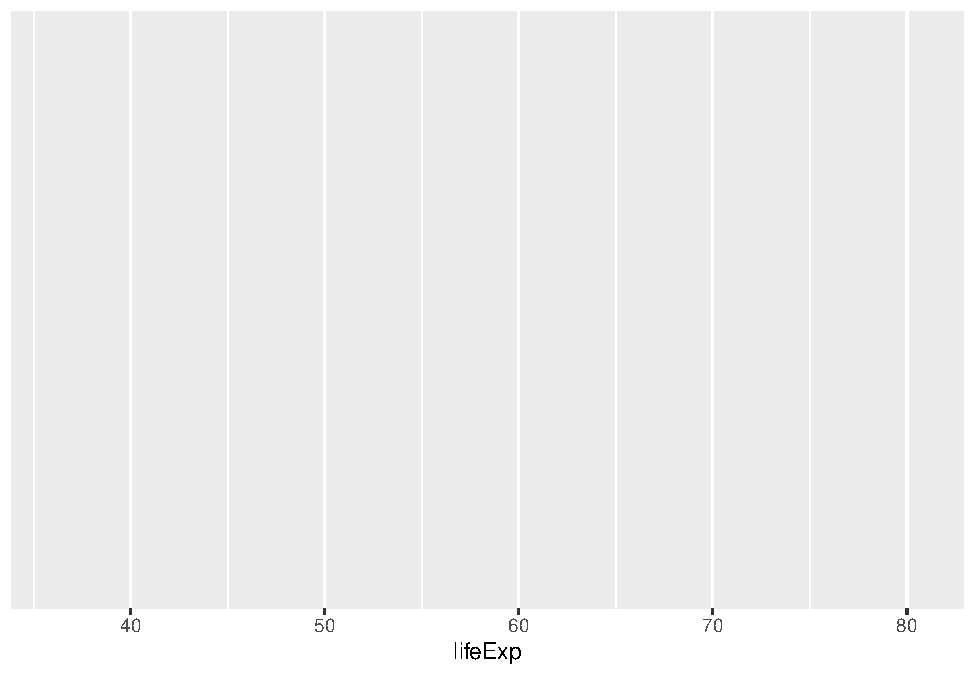
\includegraphics{bookdown-R-Essentials_files/figure-latex/unnamed-chunk-36-1.pdf}

Now we use additional code to place the dotplot in the existing
graphical region. In ggplot graphics we make graphical objects with a
\texttt{geom} function - here a dotplot so we use
\texttt{geom\_dotplot()} to produce the dotplot specified using the
variable mappings in the aesthetics command \texttt{aes} in the ggplot
command.

\begin{Shaded}
\begin{Highlighting}[]
\NormalTok{ds <-}\StringTok{ }\NormalTok{gapminder }\OperatorTok\StringTok{ }\KeywordTok{filter}\NormalTok{(year}\OperatorTok{==}\DecValTok{1997}\NormalTok{) }
\CommentTok{#}
\KeywordTok{ggplot}\NormalTok{(}\DataTypeTok{data=}\NormalTok{ds, }\DataTypeTok{mapping=}\KeywordTok{aes}\NormalTok{(}\DataTypeTok{x=}\NormalTok{lifeExp)) }\OperatorTok{+}\StringTok{ }
\StringTok{  }\KeywordTok{geom_dotplot}\NormalTok{() }\OperatorTok{+}\StringTok{ }
\StringTok{  }\KeywordTok{xlab}\NormalTok{(}\StringTok{"Life Expectancy (years)"}\NormalTok{) }\OperatorTok{+}\StringTok{ }\KeywordTok{ylab}\NormalTok{(}\StringTok{"Frequency"}\NormalTok{)}
\end{Highlighting}
\end{Shaded}

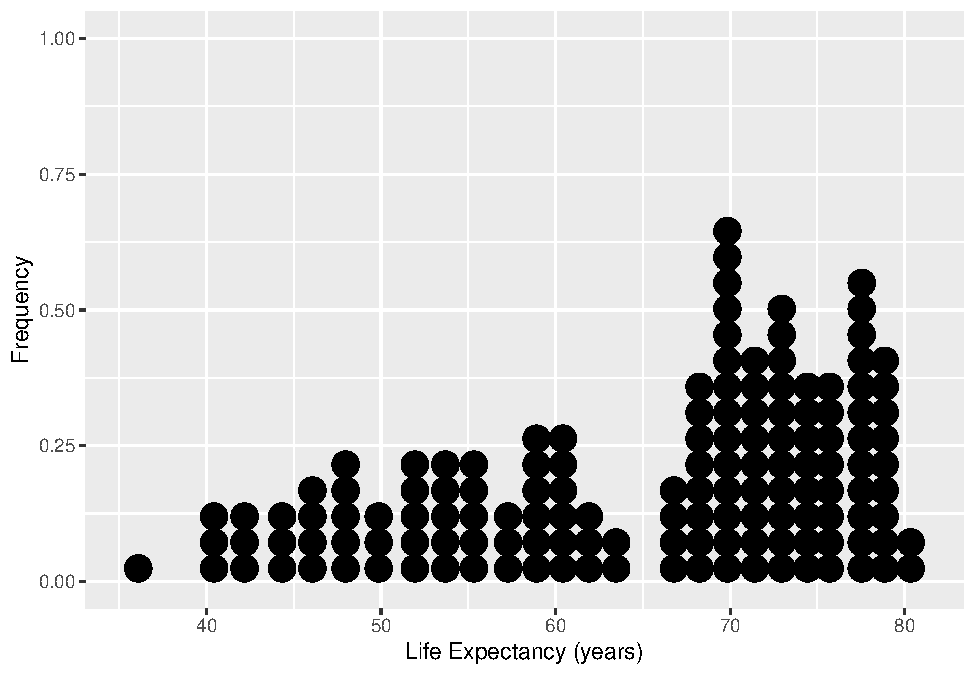
\includegraphics{bookdown-R-Essentials_files/figure-latex/unnamed-chunk-37-1.pdf}

Here we change the default size for the dots.

\begin{Shaded}
\begin{Highlighting}[]
\NormalTok{ds <-}\StringTok{ }\NormalTok{gapminder }\OperatorTok\StringTok{ }\KeywordTok{filter}\NormalTok{(year}\OperatorTok{==}\DecValTok{1997}\NormalTok{) }
\CommentTok{#}
\KeywordTok{ggplot}\NormalTok{(}\DataTypeTok{data=}\NormalTok{ds, }\DataTypeTok{mapping=}\KeywordTok{aes}\NormalTok{(}\DataTypeTok{x=}\NormalTok{lifeExp)) }\OperatorTok{+}\StringTok{ }
\StringTok{  }\KeywordTok{geom_dotplot}\NormalTok{(}\DataTypeTok{dotsize=}\FloatTok{0.70}\NormalTok{) }\OperatorTok{+}\StringTok{ }
\StringTok{  }\KeywordTok{xlab}\NormalTok{(}\StringTok{"Life Expectancy (years)"}\NormalTok{) }\OperatorTok{+}\StringTok{ }\KeywordTok{ylab}\NormalTok{(}\StringTok{"Frequency"}\NormalTok{)}
\end{Highlighting}
\end{Shaded}

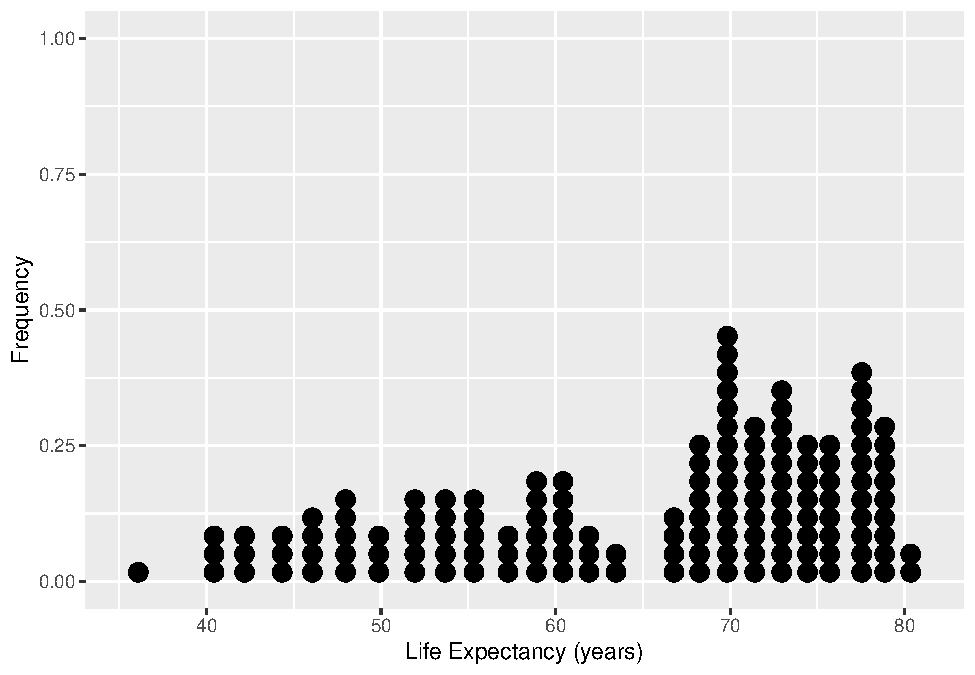
\includegraphics{bookdown-R-Essentials_files/figure-latex/unnamed-chunk-38-1.pdf}

\subsubsection{Dotplot with observations identified and
ordered}\label{dotplot-with-observations-identified-and-ordered}

Here we produce a display so that life expectancy is displayed for each
country in Asia, and the values are ordered.

\begin{Shaded}
\begin{Highlighting}[]
\NormalTok{ds <-}\StringTok{ }\NormalTok{gapminder }\OperatorTok\StringTok{ }\KeywordTok{filter}\NormalTok{(continent}\OperatorTok{==}\StringTok{"Asia"}\NormalTok{,year}\OperatorTok{==}\DecValTok{1997}\NormalTok{) }
\CommentTok{#  }
\KeywordTok{ggplot}\NormalTok{(}\DataTypeTok{data=}\NormalTok{ds, }\DataTypeTok{mapping=}\KeywordTok{aes}\NormalTok{(}\DataTypeTok{x=}\NormalTok{lifeExp, }\DataTypeTok{y=} \KeywordTok{reorder}\NormalTok{(country,lifeExp))) }\OperatorTok{+}\StringTok{ }
\StringTok{  }\KeywordTok{geom_point}\NormalTok{() }\OperatorTok{+}\StringTok{ }
\StringTok{  }\KeywordTok{xlab}\NormalTok{(}\StringTok{"Life Expectancy (years) in 1997"}\NormalTok{) }\OperatorTok{+}\StringTok{ }
\StringTok{  }\KeywordTok{ylab}\NormalTok{(}\StringTok{"Asian Countries"}\NormalTok{)}
\end{Highlighting}
\end{Shaded}

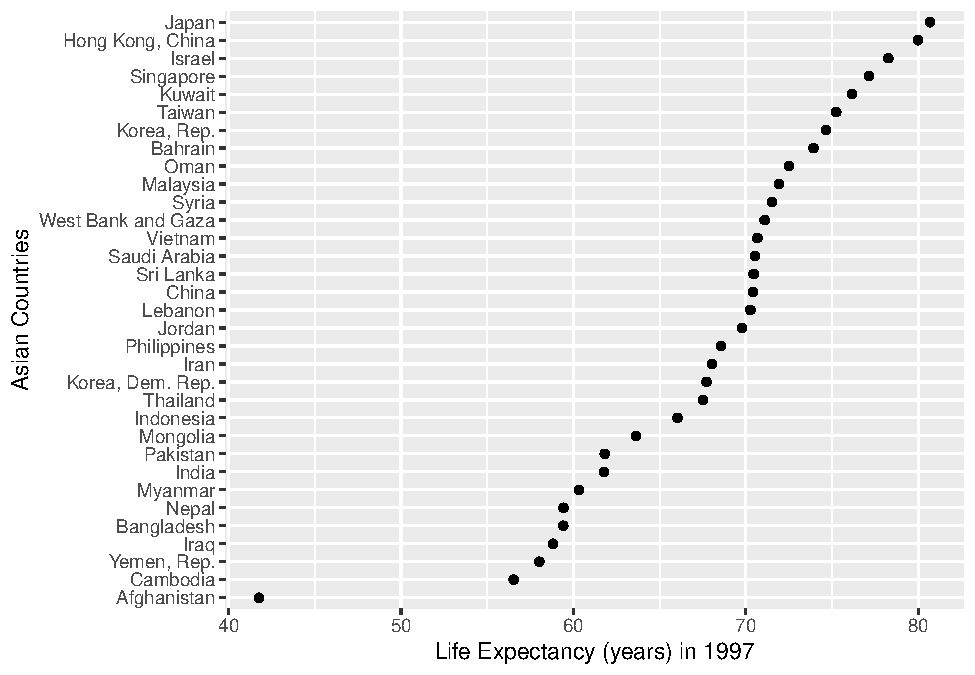
\includegraphics{bookdown-R-Essentials_files/figure-latex/unnamed-chunk-39-1.pdf}

Notice that in the next example we simply pipe the modified dataset into
the first argument of the \texttt{ggplot} command so that there is no
need to save the modified dataset to make the display.

\begin{Shaded}
\begin{Highlighting}[]
\NormalTok{gapminder }\OperatorTok\StringTok{ }\KeywordTok{filter}\NormalTok{(continent}\OperatorTok{==}\StringTok{"Asia"}\NormalTok{,year}\OperatorTok{==}\DecValTok{1997}\NormalTok{) }\OperatorTok
\KeywordTok{ggplot}\NormalTok{( }\DataTypeTok{mapping=}\KeywordTok{aes}\NormalTok{(}\DataTypeTok{x=}\NormalTok{lifeExp, }\DataTypeTok{y=} \KeywordTok{reorder}\NormalTok{(country,lifeExp))) }\OperatorTok{+}\StringTok{ }
\StringTok{  }\KeywordTok{geom_point}\NormalTok{() }\OperatorTok{+}\StringTok{ }
\StringTok{  }\KeywordTok{xlab}\NormalTok{(}\StringTok{"Life Expectancy (years) in 1997"}\NormalTok{) }\OperatorTok{+}\StringTok{ }
\StringTok{  }\KeywordTok{ylab}\NormalTok{(}\StringTok{"Asian Countries"}\NormalTok{)}
\end{Highlighting}
\end{Shaded}

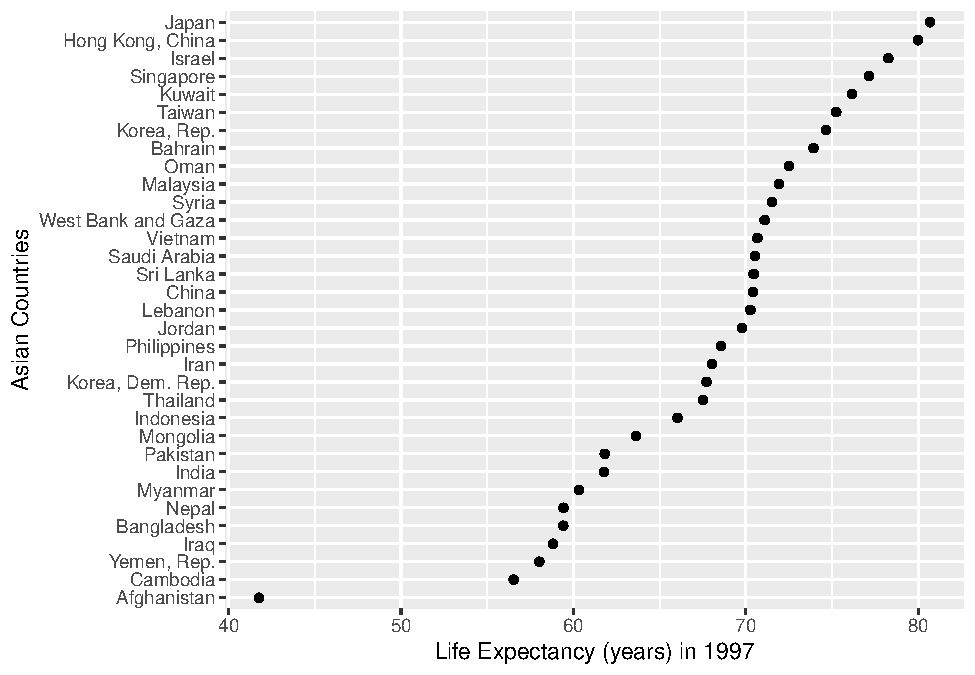
\includegraphics{bookdown-R-Essentials_files/figure-latex/unnamed-chunk-40-1.pdf}

\subsection{Histogram}\label{histogram}

This code block is similar to the dotplot commands, but the
geom\_histogram function controls the bin width in units of the x
variable - in this case 5 years.

\begin{Shaded}
\begin{Highlighting}[]
\NormalTok{gapminder }\OperatorTok\StringTok{ }\KeywordTok{filter}\NormalTok{(year}\OperatorTok{==}\DecValTok{1997}\NormalTok{) }\OperatorTok
\KeywordTok{ggplot}\NormalTok{(}\DataTypeTok{mapping=}\KeywordTok{aes}\NormalTok{(}\DataTypeTok{x=}\NormalTok{lifeExp)) }\OperatorTok{+}\StringTok{ }
\StringTok{  }\KeywordTok{geom_histogram}\NormalTok{(}\DataTypeTok{binwidth=}\DecValTok{5}\NormalTok{) }\OperatorTok{+}\StringTok{ }
\StringTok{  }\KeywordTok{xlab}\NormalTok{(}\StringTok{"Life Expectancy (years)"}\NormalTok{) }\OperatorTok{+}
\StringTok{  }\KeywordTok{ylab}\NormalTok{(}\StringTok{"Relative Frequency"}\NormalTok{)}
\end{Highlighting}
\end{Shaded}

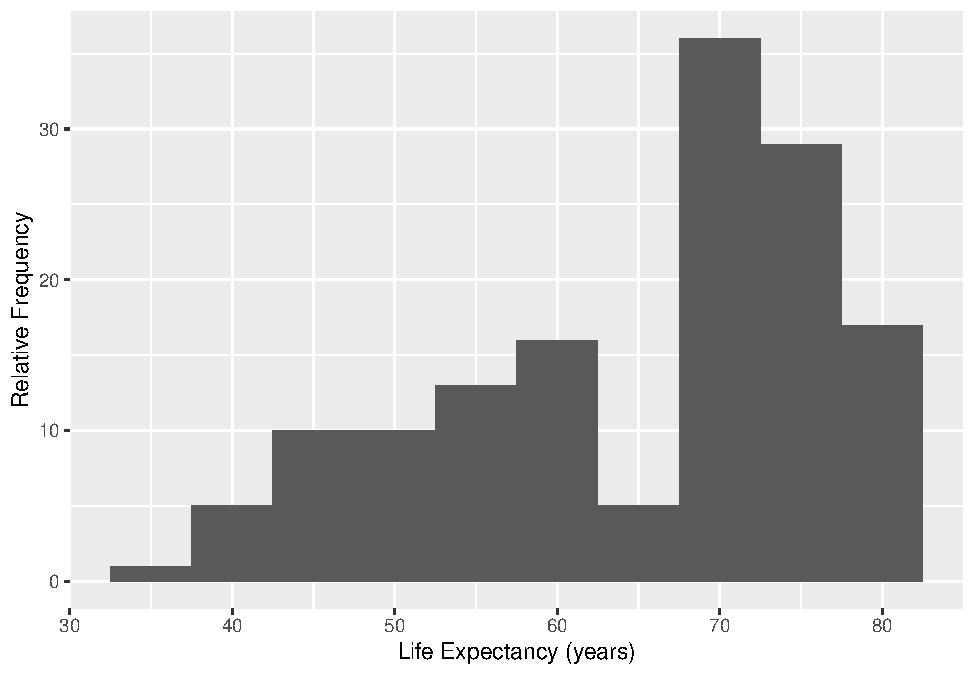
\includegraphics{bookdown-R-Essentials_files/figure-latex/unnamed-chunk-41-1.pdf}

Here we change the binwidth:

\begin{Shaded}
\begin{Highlighting}[]
\NormalTok{gapminder }\OperatorTok\StringTok{ }\KeywordTok{filter}\NormalTok{(year}\OperatorTok{==}\DecValTok{1997}\NormalTok{) }\OperatorTok
\KeywordTok{ggplot}\NormalTok{(}\DataTypeTok{mapping=}\KeywordTok{aes}\NormalTok{(}\DataTypeTok{x=}\NormalTok{lifeExp)) }\OperatorTok{+}\StringTok{ }
\StringTok{  }\KeywordTok{geom_histogram}\NormalTok{(}\DataTypeTok{binwidth=}\FloatTok{2.5}\NormalTok{) }\OperatorTok{+}\StringTok{ }
\StringTok{  }\KeywordTok{xlab}\NormalTok{(}\StringTok{"Life Expectancy (years)"}\NormalTok{) }\OperatorTok{+}
\StringTok{  }\KeywordTok{ylab}\NormalTok{(}\StringTok{"Relative Frequency"}\NormalTok{)}
\end{Highlighting}
\end{Shaded}

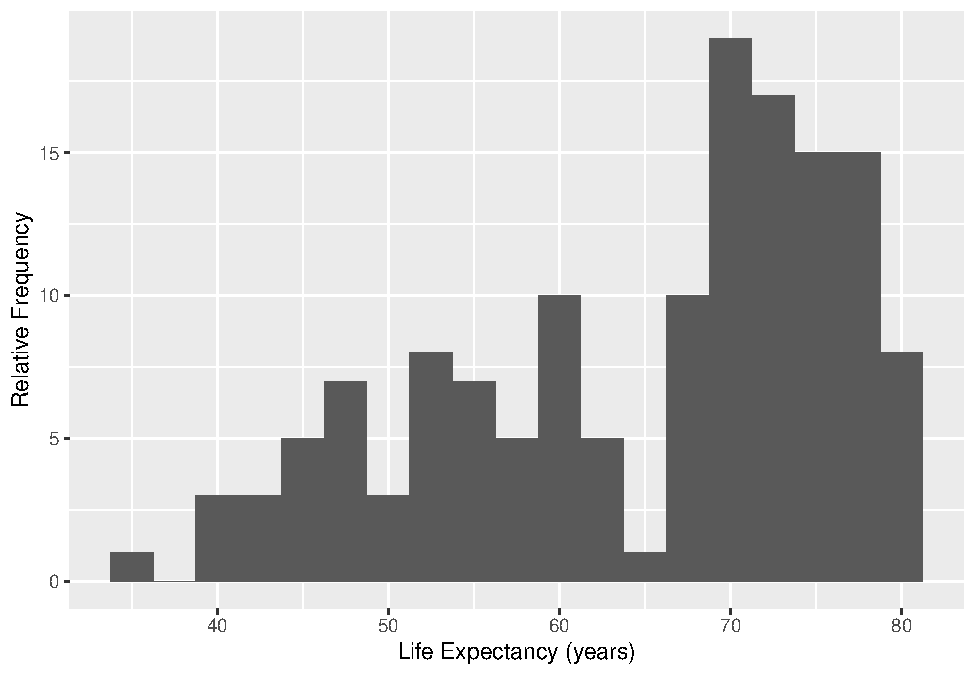
\includegraphics{bookdown-R-Essentials_files/figure-latex/unnamed-chunk-42-1.pdf}

\subsection{Density Plot}\label{density-plot}

Density plots produces a smoothing of a histogram to display the
distribution.

\begin{Shaded}
\begin{Highlighting}[]
\NormalTok{ds <-}\StringTok{ }\NormalTok{gapminder }\OperatorTok\StringTok{ }\KeywordTok{filter}\NormalTok{(year}\OperatorTok{==}\DecValTok{1997}\NormalTok{)}
\CommentTok{#}
\KeywordTok{ggplot}\NormalTok{(}\DataTypeTok{data=}\NormalTok{ds, }\DataTypeTok{mapping=}\KeywordTok{aes}\NormalTok{(}\DataTypeTok{x=}\NormalTok{lifeExp)) }\OperatorTok{+}\StringTok{ }
\StringTok{  }\KeywordTok{geom_density}\NormalTok{() }\OperatorTok{+}\StringTok{ }
\StringTok{  }\KeywordTok{xlab}\NormalTok{(}\StringTok{"Life Expectancy (years)"}\NormalTok{) }\OperatorTok{+}
\StringTok{  }\KeywordTok{ylab}\NormalTok{(}\StringTok{"Density"}\NormalTok{)}
\end{Highlighting}
\end{Shaded}

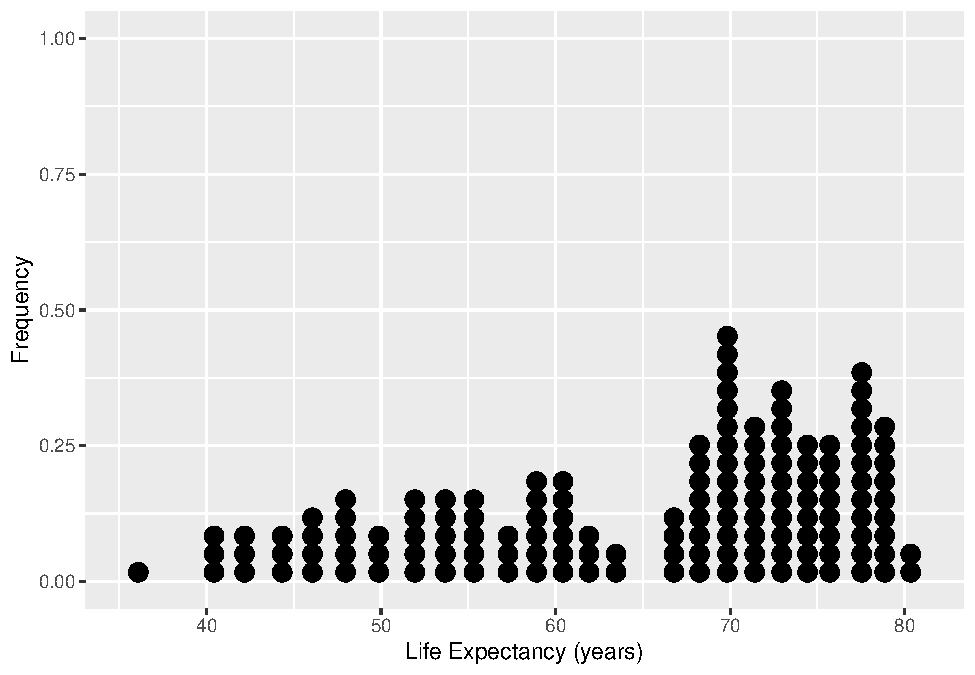
\includegraphics{bookdown-R-Essentials_files/figure-latex/unnamed-chunk-43-1.pdf}

The \texttt{adjust} option controls the amount of smoothing relative to
a default value of 1. A smaller value gives less smoothing (more
responsive line to small changes in the data distribution), and larger
values will make a smoother curve that is less sensitive to the data
pattern.

\begin{Shaded}
\begin{Highlighting}[]
\NormalTok{ds <-}\StringTok{ }\NormalTok{gapminder }\OperatorTok\StringTok{ }\KeywordTok{filter}\NormalTok{(year}\OperatorTok{==}\DecValTok{1997}\NormalTok{)}
\CommentTok{#}
\KeywordTok{ggplot}\NormalTok{(}\DataTypeTok{data=}\NormalTok{ds, }\DataTypeTok{mapping=}\KeywordTok{aes}\NormalTok{(}\DataTypeTok{x=}\NormalTok{lifeExp)) }\OperatorTok{+}\StringTok{ }
\StringTok{  }\KeywordTok{geom_density}\NormalTok{(}\DataTypeTok{adjust=}\FloatTok{0.75}\NormalTok{) }\OperatorTok{+}\StringTok{ }
\StringTok{  }\KeywordTok{xlab}\NormalTok{(}\StringTok{"Life Expectancy (years)"}\NormalTok{) }\OperatorTok{+}
\StringTok{  }\KeywordTok{ylab}\NormalTok{(}\StringTok{"Density"}\NormalTok{)}
\end{Highlighting}
\end{Shaded}

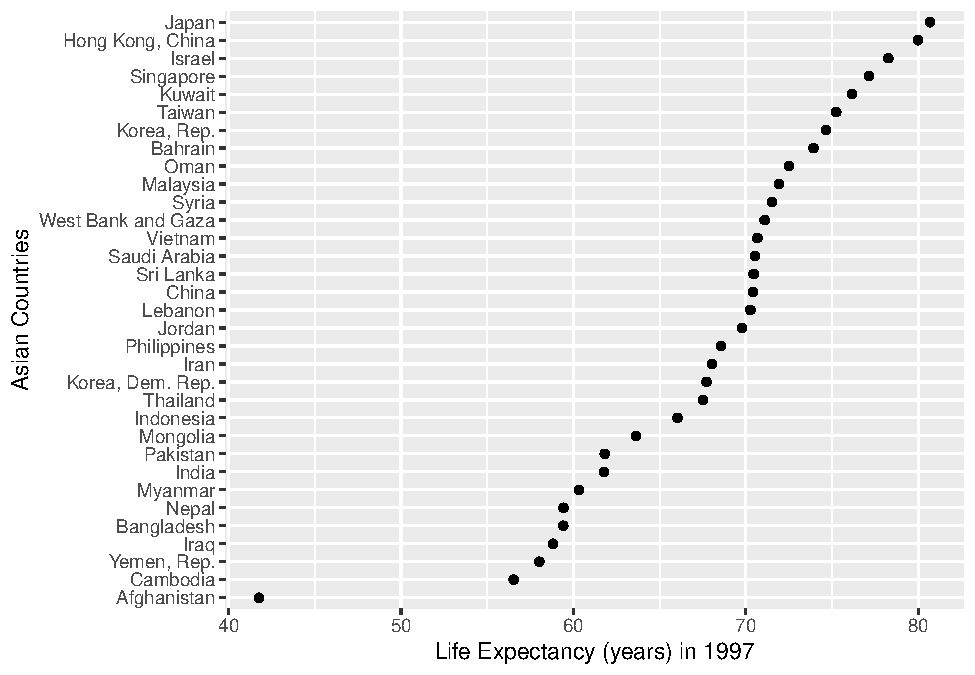
\includegraphics{bookdown-R-Essentials_files/figure-latex/unnamed-chunk-44-1.pdf}

\subsection{Boxplot}\label{boxplot}

The boxplot display really needs only a single quantitative variable
(here life expectancy) for the numeric axis. However, the other axis
looks better with some sort of factor variable - so here we supply the
year for the display, where the quantitative variable \texttt{year} has
temporarily being used as a category/factor variable by being processed
by the \texttt{factor} function before used in the graphic:

\begin{Shaded}
\begin{Highlighting}[]
\NormalTok{ds <-}\StringTok{ }\NormalTok{gapminder }\OperatorTok\StringTok{ }\KeywordTok{filter}\NormalTok{(year}\OperatorTok{==}\DecValTok{1997}\NormalTok{) }
\CommentTok{#}
\KeywordTok{ggplot}\NormalTok{(}\DataTypeTok{data=}\NormalTok{ds, }\DataTypeTok{mapping=}\KeywordTok{aes}\NormalTok{(}\DataTypeTok{x=}\KeywordTok{factor}\NormalTok{(year),}\DataTypeTok{y=}\NormalTok{lifeExp)) }\OperatorTok{+}
\StringTok{ }\KeywordTok{geom_boxplot}\NormalTok{() }\OperatorTok{+}\StringTok{ }
\StringTok{  }\KeywordTok{labs}\NormalTok{(}\DataTypeTok{x=}\StringTok{"Year"}\NormalTok{,}\DataTypeTok{y=}\StringTok{"Life Expectancy (years)"}\NormalTok{)}
\end{Highlighting}
\end{Shaded}

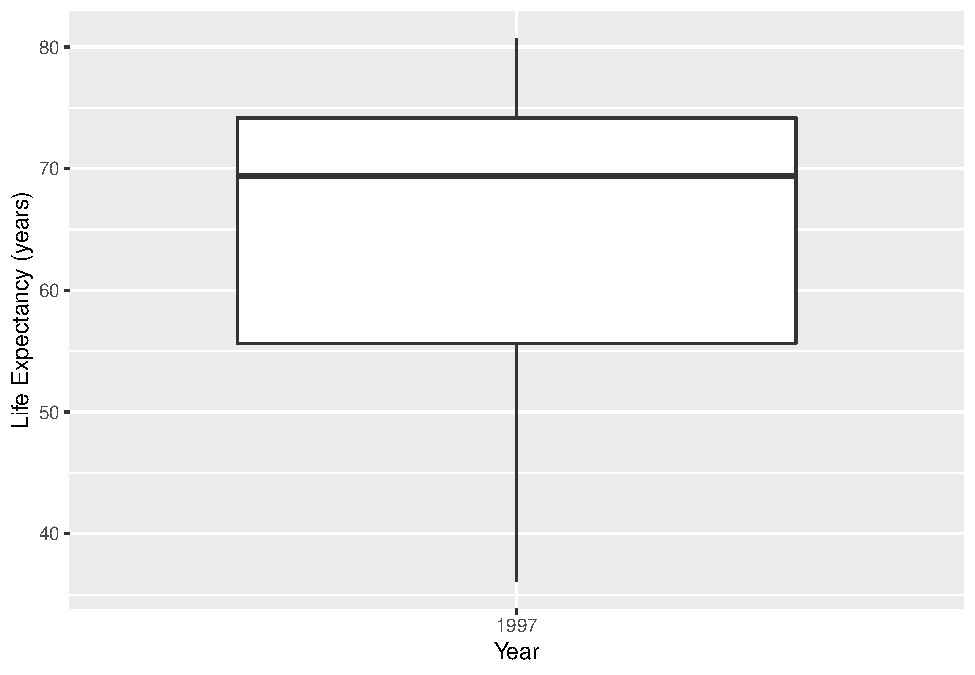
\includegraphics{bookdown-R-Essentials_files/figure-latex/unnamed-chunk-45-1.pdf}

\begin{Shaded}
\begin{Highlighting}[]
\CommentTok{# Change orientation}
\KeywordTok{ggplot}\NormalTok{(}\DataTypeTok{data=}\NormalTok{ds, }\DataTypeTok{mapping=}\KeywordTok{aes}\NormalTok{(}\DataTypeTok{x=}\KeywordTok{factor}\NormalTok{(year),}\DataTypeTok{y=}\NormalTok{lifeExp)) }\OperatorTok{+}
\StringTok{ }\KeywordTok{geom_boxplot}\NormalTok{() }\OperatorTok{+}\StringTok{ }
\StringTok{  }\KeywordTok{coord_flip}\NormalTok{() }\OperatorTok{+}\StringTok{ }
\StringTok{  }\KeywordTok{labs}\NormalTok{(}\DataTypeTok{x=}\StringTok{"Year"}\NormalTok{,}\DataTypeTok{y=}\StringTok{"Life Expectancy (years)"}\NormalTok{)}
\end{Highlighting}
\end{Shaded}

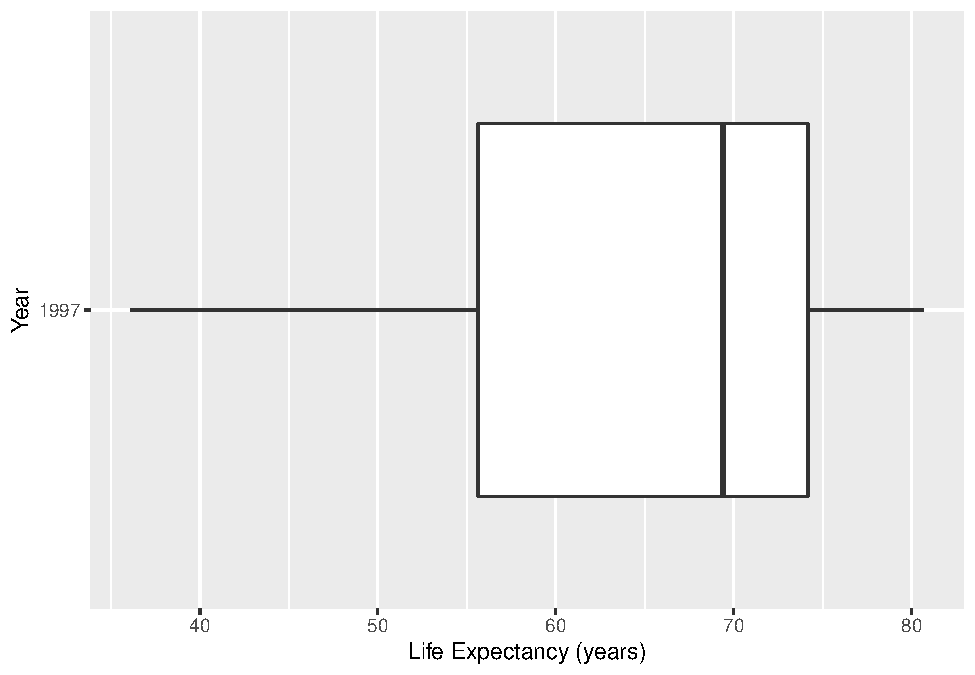
\includegraphics{bookdown-R-Essentials_files/figure-latex/unnamed-chunk-45-2.pdf}

Now we overlay points on top of the boxplot display. Note the
\texttt{geom\_jitter} that overlays the points has an argument
\texttt{alpha=0.5} signifying a slightly transparent plot symbol. An
alpha value of 1 means the plot symbol is opaque, and a value of 0 is
comletely transparent. Careful use of alpha in large datasets will
enable the analyst to correctly perceive point density. Without using a
smaller value of \texttt{alpha} the plot may be one large blob of ink -
making it difficult to judge the density of points in the display.

\begin{Shaded}
\begin{Highlighting}[]
\NormalTok{ds <-}\StringTok{ }\NormalTok{gapminder }\OperatorTok\StringTok{ }\KeywordTok{filter}\NormalTok{(year}\OperatorTok{==}\DecValTok{1997}\NormalTok{) }
\CommentTok{#}
\KeywordTok{ggplot}\NormalTok{(}\DataTypeTok{data=}\NormalTok{ds, }\DataTypeTok{mapping=}\KeywordTok{aes}\NormalTok{(}\DataTypeTok{x=}\KeywordTok{factor}\NormalTok{(year),}\DataTypeTok{y=}\NormalTok{lifeExp)) }\OperatorTok{+}
\StringTok{ }\KeywordTok{geom_boxplot}\NormalTok{(}\DataTypeTok{outlier.shape =} \OtherTok{NA}\NormalTok{) }\OperatorTok{+}\StringTok{ }
\StringTok{ }\KeywordTok{geom_jitter}\NormalTok{(}\DataTypeTok{alpha=}\FloatTok{0.5}\NormalTok{, }\DataTypeTok{width=}\FloatTok{0.35}\NormalTok{) }\OperatorTok{+}
\StringTok{  }\KeywordTok{labs}\NormalTok{(}\DataTypeTok{x=}\StringTok{"Year"}\NormalTok{,}\DataTypeTok{y=}\StringTok{"Life Expectancy (years)"}\NormalTok{)}
\end{Highlighting}
\end{Shaded}

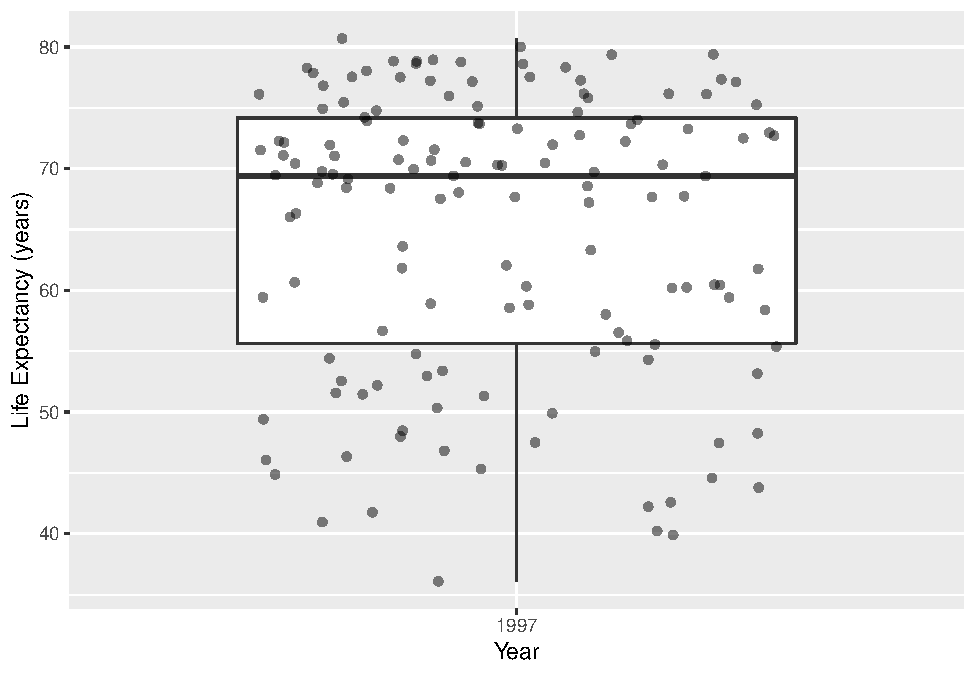
\includegraphics{bookdown-R-Essentials_files/figure-latex/unnamed-chunk-46-1.pdf}

If the dataframe has only one quantitative variable, we can make a
character variable called ``sample'', then this code will produce an
acceptable display.

\begin{Shaded}
\begin{Highlighting}[]
\NormalTok{ds <-}\StringTok{ }\NormalTok{gapminder }\OperatorTok\StringTok{ }\KeywordTok{filter}\NormalTok{(year}\OperatorTok{==}\DecValTok{1997}\NormalTok{) }\OperatorTok
\StringTok{  }\KeywordTok{mutate}\NormalTok{(}\DataTypeTok{sample=}\StringTok{"Sample"}\NormalTok{)}
\CommentTok{#}
\KeywordTok{ggplot}\NormalTok{(}\DataTypeTok{data=}\NormalTok{ds, }\DataTypeTok{mapping=}\KeywordTok{aes}\NormalTok{(}\DataTypeTok{x=}\NormalTok{sample,}\DataTypeTok{y=}\NormalTok{lifeExp)) }\OperatorTok{+}
\StringTok{ }\KeywordTok{geom_boxplot}\NormalTok{(}\DataTypeTok{outlier.shape =} \OtherTok{NA}\NormalTok{) }\OperatorTok{+}\StringTok{ }
\StringTok{ }\KeywordTok{geom_jitter}\NormalTok{(}\DataTypeTok{alpha=}\FloatTok{0.5}\NormalTok{, }\DataTypeTok{width=}\FloatTok{0.35}\NormalTok{) }\OperatorTok{+}
\StringTok{  }\KeywordTok{labs}\NormalTok{(}\DataTypeTok{x=}\StringTok{""}\NormalTok{,}\DataTypeTok{y=}\StringTok{"Life Expectancy (years)"}\NormalTok{)}
\end{Highlighting}
\end{Shaded}

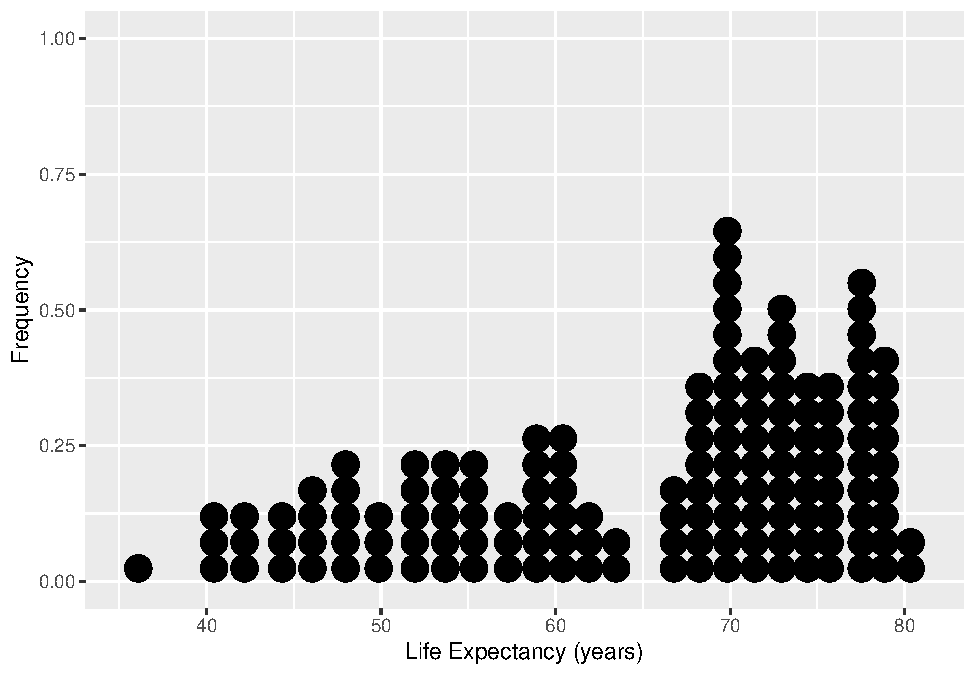
\includegraphics{bookdown-R-Essentials_files/figure-latex/unnamed-chunk-47-1.pdf}

\section{Displays of a Categorical
Variable}\label{displays-of-a-categorical-variable}

\subsection{Bar Graph}\label{bar-graph}

\begin{Shaded}
\begin{Highlighting}[]
\NormalTok{ds <-}\StringTok{ }\NormalTok{gapminder }\OperatorTok\StringTok{ }
\StringTok{  }\KeywordTok{filter}\NormalTok{(year}\OperatorTok{==}\DecValTok{1997}\NormalTok{) }\OperatorTok\StringTok{ }
\StringTok{  }\KeywordTok{group_by}\NormalTok{(continent) }
\CommentTok{# Frequency of countries in each continent in 1997.}
\KeywordTok{ggplot}\NormalTok{(}\DataTypeTok{data=}\NormalTok{ds, }\DataTypeTok{mapping=}\KeywordTok{aes}\NormalTok{(}\DataTypeTok{x=}\NormalTok{continent)) }\OperatorTok{+}\StringTok{ }
\StringTok{  }\KeywordTok{geom_bar}\NormalTok{() }\OperatorTok{+}
\StringTok{  }\KeywordTok{labs}\NormalTok{(}\DataTypeTok{x=}\StringTok{"Continent"}\NormalTok{, }\DataTypeTok{y=}\StringTok{"Frequency"}\NormalTok{)}
\end{Highlighting}
\end{Shaded}

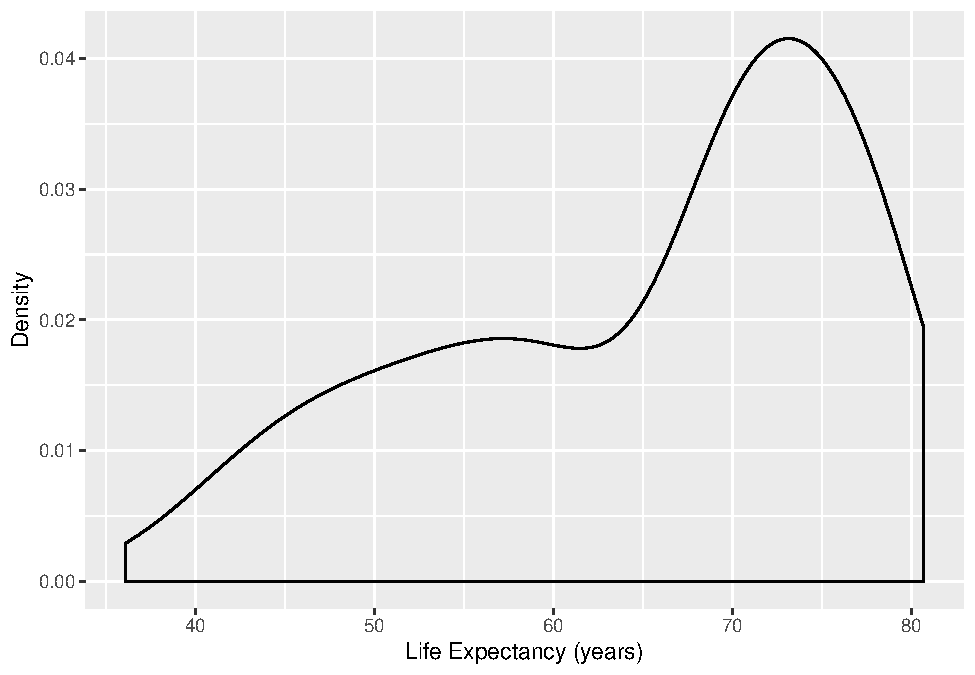
\includegraphics{bookdown-R-Essentials_files/figure-latex/unnamed-chunk-48-1.pdf}

\begin{Shaded}
\begin{Highlighting}[]
\CommentTok{#}
\KeywordTok{ggplot}\NormalTok{(}\DataTypeTok{data=}\NormalTok{ds, }\DataTypeTok{mapping=}\KeywordTok{aes}\NormalTok{(}\DataTypeTok{x=}\NormalTok{continent)) }\OperatorTok{+}\StringTok{ }
\StringTok{  }\KeywordTok{geom_bar}\NormalTok{(}\DataTypeTok{width=}\FloatTok{0.5}\NormalTok{,}\DataTypeTok{fill=}\StringTok{"blue"}\NormalTok{) }\OperatorTok{+}
\StringTok{  }\KeywordTok{labs}\NormalTok{(}\DataTypeTok{title=}\StringTok{"Countries in Each Continent"}\NormalTok{,}
       \DataTypeTok{subtitle =} \StringTok{"Year = 1997"}\NormalTok{,}
       \DataTypeTok{caption =} \StringTok{"Gapminder data"}\NormalTok{,}
       \DataTypeTok{x=}\StringTok{"Continent"}\NormalTok{, }
       \DataTypeTok{y=}\StringTok{"Frequency"}\NormalTok{) }\OperatorTok{+}
\StringTok{  }\KeywordTok{theme}\NormalTok{(}\DataTypeTok{axis.text.x =} \KeywordTok{element_text}\NormalTok{(}\DataTypeTok{angle=}\DecValTok{45}\NormalTok{,}\DataTypeTok{vjust =} \FloatTok{0.6}\NormalTok{))}
\end{Highlighting}
\end{Shaded}

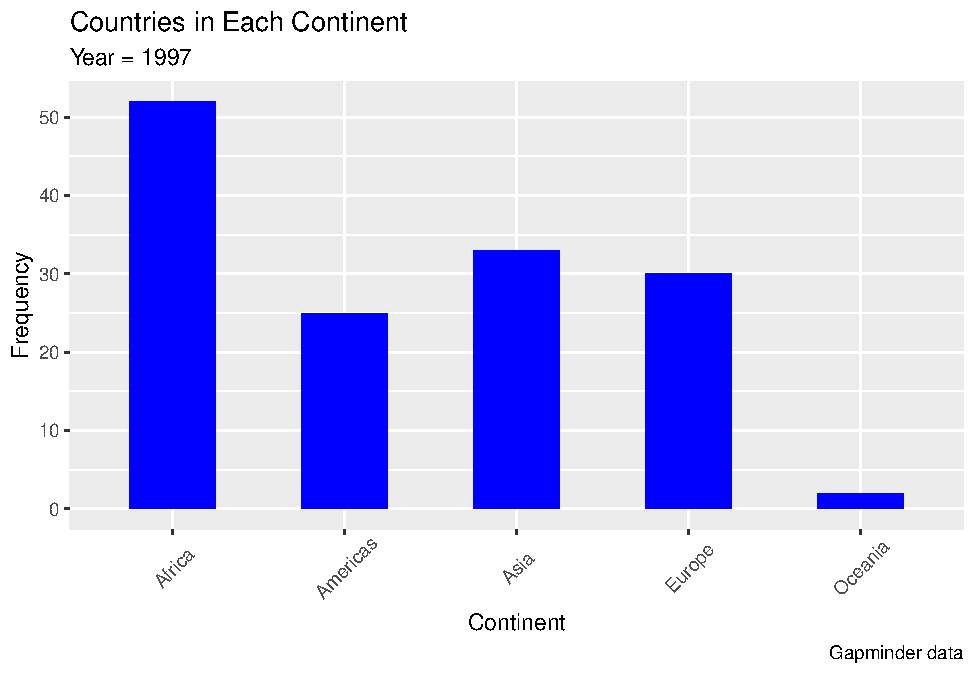
\includegraphics{bookdown-R-Essentials_files/figure-latex/unnamed-chunk-48-2.pdf}

Bar graph with percentages on vertical axis.

\begin{Shaded}
\begin{Highlighting}[]
\NormalTok{ds <-}\StringTok{ }\NormalTok{gapminder }\OperatorTok\StringTok{ }
\StringTok{  }\KeywordTok{filter}\NormalTok{(year}\OperatorTok{==}\DecValTok{1997}\NormalTok{) }\OperatorTok\StringTok{ }
\StringTok{  }\KeywordTok{group_by}\NormalTok{(continent)  }\OperatorTok
\StringTok{  }\KeywordTok{summarise}\NormalTok{ (}\DataTypeTok{n =} \KeywordTok{n}\NormalTok{()) }\OperatorTok
\StringTok{  }\KeywordTok{mutate}\NormalTok{(}\DataTypeTok{pct =} \DecValTok{100}\OperatorTok{*}\NormalTok{n }\OperatorTok{/}\StringTok{ }\KeywordTok{sum}\NormalTok{(n)) }
\CommentTok{#}
\KeywordTok{ggplot}\NormalTok{(}\DataTypeTok{data=}\NormalTok{ds, }\DataTypeTok{mapping=}\KeywordTok{aes}\NormalTok{(}\DataTypeTok{x =}\NormalTok{ continent, }\DataTypeTok{y =}\NormalTok{ pct)) }\OperatorTok{+}\StringTok{ }
\StringTok{  }\KeywordTok{geom_bar}\NormalTok{(}\DataTypeTok{stat =} \StringTok{"identity"}\NormalTok{) }\OperatorTok{+}\StringTok{ }
\StringTok{  }\KeywordTok{xlab}\NormalTok{(}\StringTok{"Continent"}\NormalTok{) }\OperatorTok{+}\StringTok{ }\KeywordTok{ylab}\NormalTok{(}\StringTok{"Percentage"}\NormalTok{)}
\end{Highlighting}
\end{Shaded}

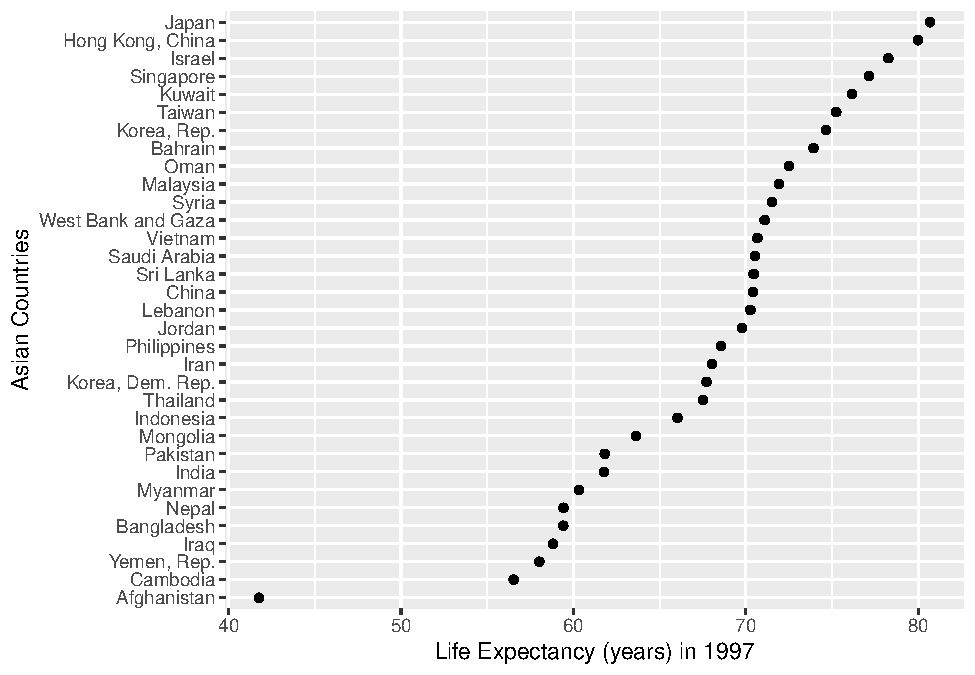
\includegraphics{bookdown-R-Essentials_files/figure-latex/unnamed-chunk-49-1.pdf}

\begin{Shaded}
\begin{Highlighting}[]
\CommentTok{# change order of continents in decreasing frequency order}
\KeywordTok{ggplot}\NormalTok{(}\DataTypeTok{data=}\NormalTok{ds, }\DataTypeTok{mapping=}\KeywordTok{aes}\NormalTok{(}\DataTypeTok{x =} \KeywordTok{reorder}\NormalTok{(continent, }\OperatorTok{-}\NormalTok{pct), }\DataTypeTok{y =}\NormalTok{ pct)) }\OperatorTok{+}\StringTok{ }
\StringTok{  }\KeywordTok{geom_bar}\NormalTok{(}\DataTypeTok{stat =} \StringTok{"identity"}\NormalTok{) }\OperatorTok{+}\StringTok{ }
\StringTok{  }\KeywordTok{xlab}\NormalTok{(}\StringTok{"Continent"}\NormalTok{) }\OperatorTok{+}\StringTok{ }\KeywordTok{ylab}\NormalTok{(}\StringTok{"Percentage"}\NormalTok{)}
\end{Highlighting}
\end{Shaded}

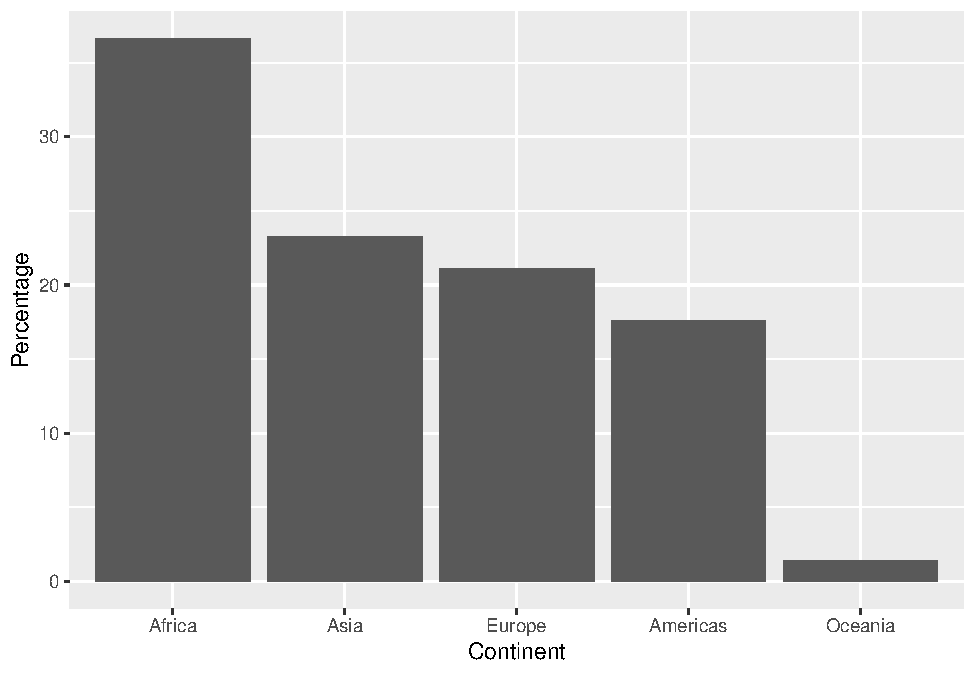
\includegraphics{bookdown-R-Essentials_files/figure-latex/unnamed-chunk-49-2.pdf}

Sometimes it is more convenient to have the bars oriented horizontally.
Notice we set up the aesthetic mappings as usual and then flip the axes
with the \texttt{coord\_flip} command.

\begin{Shaded}
\begin{Highlighting}[]
\NormalTok{ds <-}\StringTok{ }\NormalTok{gapminder }\OperatorTok\StringTok{ }
\StringTok{  }\KeywordTok{filter}\NormalTok{(year}\OperatorTok{==}\DecValTok{1997}\NormalTok{) }\OperatorTok\StringTok{ }
\StringTok{  }\KeywordTok{group_by}\NormalTok{(continent)  }\OperatorTok
\StringTok{  }\KeywordTok{summarise}\NormalTok{ (}\DataTypeTok{n =} \KeywordTok{n}\NormalTok{()) }\OperatorTok
\StringTok{  }\KeywordTok{mutate}\NormalTok{(}\DataTypeTok{pct =} \DecValTok{100}\OperatorTok{*}\NormalTok{n }\OperatorTok{/}\StringTok{ }\KeywordTok{sum}\NormalTok{(n)) }
\CommentTok{#}
\KeywordTok{ggplot}\NormalTok{(}\DataTypeTok{data=}\NormalTok{ds, }\DataTypeTok{mapping=}\KeywordTok{aes}\NormalTok{(}\DataTypeTok{x =} \KeywordTok{reorder}\NormalTok{(continent, pct), }\DataTypeTok{y =}\NormalTok{ pct)) }\OperatorTok{+}\StringTok{ }
\StringTok{  }\KeywordTok{geom_bar}\NormalTok{(}\DataTypeTok{stat =} \StringTok{"identity"}\NormalTok{) }\OperatorTok{+}
\StringTok{  }\KeywordTok{coord_flip}\NormalTok{() }\OperatorTok{+}
\StringTok{  }\KeywordTok{xlab}\NormalTok{(}\StringTok{"Continent"}\NormalTok{) }\OperatorTok{+}\StringTok{ }\KeywordTok{ylab}\NormalTok{(}\StringTok{"Percentage"}\NormalTok{)}
\end{Highlighting}
\end{Shaded}

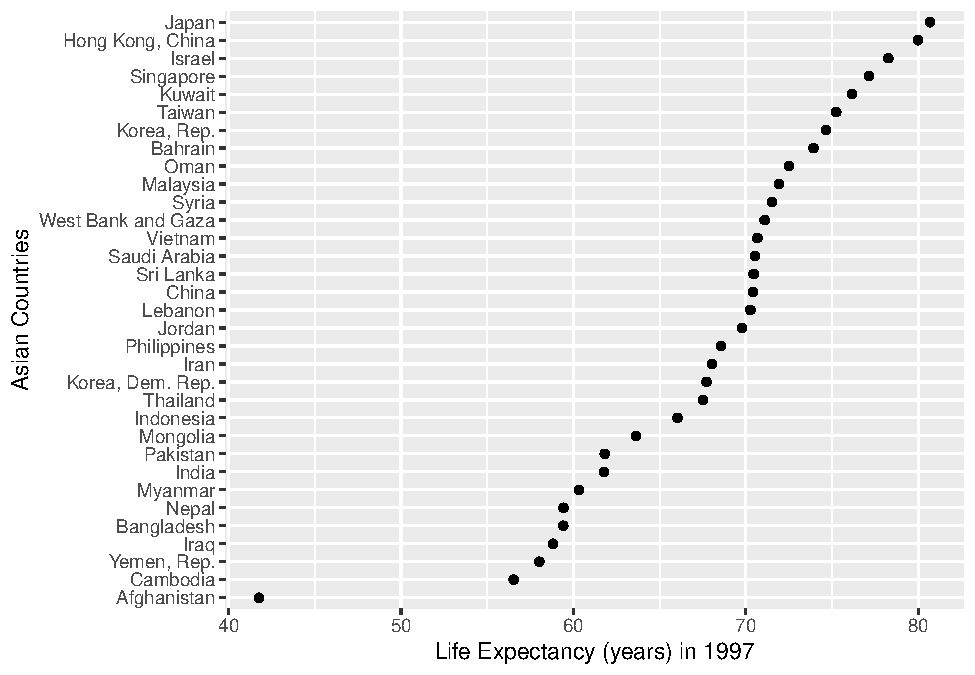
\includegraphics{bookdown-R-Essentials_files/figure-latex/unnamed-chunk-50-1.pdf}

\subsection{Pie Graph}\label{pie-graph}

Pie graphs are not recommended, but the code needed to make one is given
here.

\begin{Shaded}
\begin{Highlighting}[]
\NormalTok{contin.prop<-}\StringTok{ }\NormalTok{gapminder }\OperatorTok\StringTok{ }
\StringTok{  }\KeywordTok{group_by}\NormalTok{(continent) }\OperatorTok
\StringTok{  }\KeywordTok{summarise}\NormalTok{ (}\DataTypeTok{n =} \KeywordTok{n}\NormalTok{()) }\OperatorTok
\StringTok{  }\KeywordTok{mutate}\NormalTok{(}\DataTypeTok{freq =}\NormalTok{ n }\OperatorTok{/}\StringTok{ }\KeywordTok{sum}\NormalTok{(n))}
\CommentTok{#}
\KeywordTok{ggplot}\NormalTok{(}\DataTypeTok{data=}\NormalTok{contin.prop, }\DataTypeTok{mapping=}\KeywordTok{aes}\NormalTok{(}\DataTypeTok{x=}\StringTok{""}\NormalTok{,}\DataTypeTok{y=}\NormalTok{freq,}\DataTypeTok{fill=}\NormalTok{continent)) }\OperatorTok{+}\StringTok{ }
\StringTok{  }\KeywordTok{geom_bar}\NormalTok{(}\DataTypeTok{width=}\DecValTok{1}\NormalTok{,}\DataTypeTok{stat=}\StringTok{"identity"}\NormalTok{) }\OperatorTok{+}
\StringTok{  }\KeywordTok{coord_polar}\NormalTok{(}\StringTok{"y"}\NormalTok{,}\DataTypeTok{start=}\DecValTok{0}\NormalTok{) }\OperatorTok{+}
\StringTok{  }\KeywordTok{xlab}\NormalTok{(}\StringTok{""}\NormalTok{) }\OperatorTok{+}\StringTok{ }\KeywordTok{ylab}\NormalTok{(}\StringTok{"Country Frequency by Continent"}\NormalTok{)}
\end{Highlighting}
\end{Shaded}

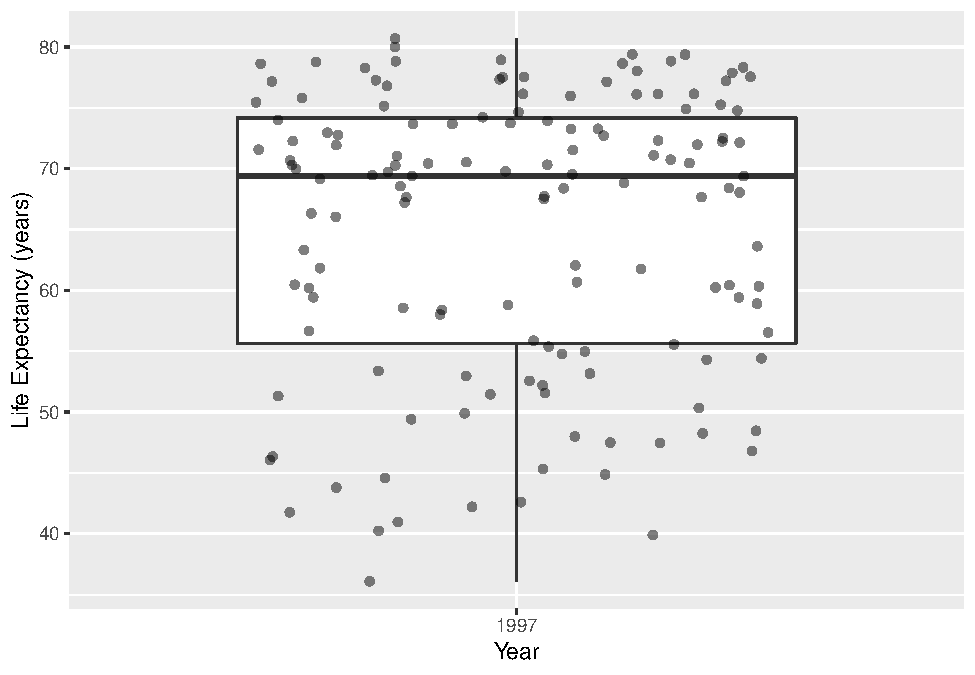
\includegraphics{bookdown-R-Essentials_files/figure-latex/unnamed-chunk-51-1.pdf}

\chapter{Summary Statistics For One
Variable}\label{summary-statistics-for-one-variable}

\section{One Quantitative Variable}\label{one-quantitative-variable}

\subsection{Using base R summary
function}\label{using-base-r-summary-function}

\begin{Shaded}
\begin{Highlighting}[]
\NormalTok{gapminder }\OperatorTok\StringTok{ }\KeywordTok{filter}\NormalTok{(year}\OperatorTok{==}\DecValTok{1997}\NormalTok{) }\OperatorTok\StringTok{ }\KeywordTok{select}\NormalTok{(lifeExp) }\OperatorTok\StringTok{ }\KeywordTok{summary}\NormalTok{()}
\end{Highlighting}
\end{Shaded}

\begin{verbatim}
##     lifeExp     
##  Min.   :36.09  
##  1st Qu.:55.63  
##  Median :69.39  
##  Mean   :65.01  
##  3rd Qu.:74.17  
##  Max.   :80.69
\end{verbatim}

\subsection{Using dplyr summarise
function}\label{using-dplyr-summarise-function}

It is often helpful to create data summaries during preliminary phases
of examination. Here is how to use the summarise command in the analysis
pipeline system.

\begin{Shaded}
\begin{Highlighting}[]
\NormalTok{gapminder }\OperatorTok\StringTok{ }\KeywordTok{filter}\NormalTok{(year}\OperatorTok{==}\DecValTok{1997}\NormalTok{) }\OperatorTok\StringTok{ }
\StringTok{      }\NormalTok{dplyr}\OperatorTok{::}\KeywordTok{summarise}\NormalTok{(}\DataTypeTok{meanLE=}\KeywordTok{mean}\NormalTok{(lifeExp,}\DataTypeTok{na.rm=}\OtherTok{TRUE}\NormalTok{),}
                       \DataTypeTok{medLE=}\KeywordTok{median}\NormalTok{(lifeExp,}\DataTypeTok{na.rm=}\OtherTok{TRUE}\NormalTok{),}
                       \DataTypeTok{sd=}\KeywordTok{sd}\NormalTok{(lifeExp,}\DataTypeTok{na.rm=}\OtherTok{TRUE}\NormalTok{),}
                       \DataTypeTok{iqr=}\KeywordTok{IQR}\NormalTok{(lifeExp,}\DataTypeTok{na.rm=}\OtherTok{TRUE}\NormalTok{),}
                      \DataTypeTok{Q1=}\KeywordTok{quantile}\NormalTok{(lifeExp,}\DataTypeTok{probs=}\FloatTok{0.25}\NormalTok{,}\DataTypeTok{na.rm=}\OtherTok{TRUE}\NormalTok{),}
                      \DataTypeTok{Q3=}\KeywordTok{quantile}\NormalTok{(lifeExp,}\DataTypeTok{probs=}\FloatTok{0.75}\NormalTok{),}
                      \DataTypeTok{n=}\KeywordTok{n}\NormalTok{())}
\end{Highlighting}
\end{Shaded}

\begin{verbatim}
## # A tibble: 1 x 7
##   meanLE medLE    sd   iqr    Q1    Q3     n
##    <dbl> <dbl> <dbl> <dbl> <dbl> <dbl> <int>
## 1   65.0  69.4  11.6  18.5  55.6  74.2   142
\end{verbatim}

\subsection{Summary Statistics Using funModeling
package}\label{summary-statistics-using-funmodeling-package}

The \texttt{profiling\_num} and \texttt{plot\_num} functions from the
\emph{funModeling} package help give a concise numeric and visual
overview of the numeric variables in the dataframe.

\begin{Shaded}
\begin{Highlighting}[]
\NormalTok{funModeling}\OperatorTok{::}\KeywordTok{profiling_num}\NormalTok{(gapminder)}
\end{Highlighting}
\end{Shaded}

\begin{verbatim}
##    variable         mean      std_dev variation_coef        p_01        p_05
## 1      year 1.979500e+03 1.726533e+01    0.008722066   1952.0000   1952.0000
## 2   lifeExp 5.947444e+01 1.291711e+01    0.217187544     33.4926     38.4924
## 3       pop 2.960121e+07 1.061579e+08    3.586268548 154117.9200 475458.9000
## 4 gdpPercap 7.215327e+03 9.857455e+03    1.366182632    369.2201    547.9964
##          p_25         p_50         p_75         p_95         p_99   skewness
## 1    1965.750    1979.5000 1.993250e+03     2007.000 2.007000e+03  0.0000000
## 2      48.198      60.7125 7.084550e+01       77.437 8.023892e+01 -0.2524798
## 3 2793664.000 7023595.5000 1.958522e+07 89822054.500 6.319900e+08  8.3328742
## 4    1202.060    3531.8470 9.325462e+03    26608.333 3.678357e+04  3.8468819
##    kurtosis          iqr                       range_98
## 1  1.783217 2.750000e+01                   [1952, 2007]
## 2  1.873099 2.264750e+01            [33.4926, 80.23892]
## 3 80.716151 1.679156e+07  [154117.92, 631990000.000002]
## 4 30.431702 8.123402e+03 [369.220127794, 36783.5723707]
##                       range_80
## 1                 [1957, 2002]
## 2            [41.5108, 75.097]
## 3       [946367.1, 54801369.5]
## 4 [687.71836128, 19449.138209]
\end{verbatim}

\begin{Shaded}
\begin{Highlighting}[]
\NormalTok{funModeling}\OperatorTok{::}\KeywordTok{plot_num}\NormalTok{(gapminder)}
\end{Highlighting}
\end{Shaded}

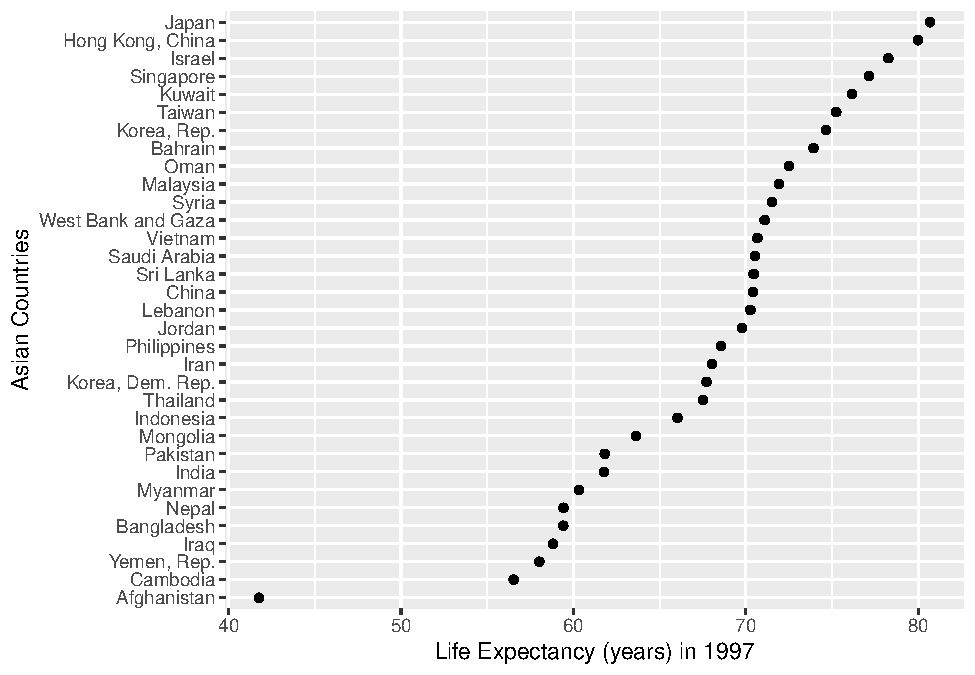
\includegraphics{bookdown-R-Essentials_files/figure-latex/unnamed-chunk-55-1.pdf}

This example shows summary statistics for two quantitative variables.
For only one variable, simply use \texttt{select} for only one variable.

\begin{Shaded}
\begin{Highlighting}[]
\NormalTok{gapminder }\OperatorTok
\StringTok{  }\KeywordTok{filter}\NormalTok{(year}\OperatorTok{==}\DecValTok{1997}\NormalTok{) }\OperatorTok
\StringTok{  }\KeywordTok{select}\NormalTok{(lifeExp,gdpPercap) }\OperatorTok
\NormalTok{funModeling}\OperatorTok{::}\KeywordTok{profiling_num}\NormalTok{() }
\end{Highlighting}
\end{Shaded}

\begin{verbatim}
##    variable       mean     std_dev variation_coef      p_01      p_05
## 1   lifeExp   65.01468    11.55944      0.1777974  40.03681  43.83415
## 2 gdpPercap 9090.17536 10171.49326      1.1189546 434.72721 590.90598
##         p_25     p_50        p_75       p_95       p_99   skewness kurtosis
## 1   55.63375   69.394    74.16975    78.7635    79.7499 -0.6427906 2.218599
## 2 1366.83796 4781.825 12022.86719 29088.8709 38442.0133  1.2979366 3.604446
##         iqr                       range_98                     range_80
## 1    18.536            [40.03681, 79.7499]            [47.4671, 77.548]
## 2 10656.029 [434.727210598, 38442.0133187] [789.29339925, 26905.596049]
\end{verbatim}

\begin{Shaded}
\begin{Highlighting}[]
\CommentTok{#}
\NormalTok{gapminder }\OperatorTok
\StringTok{  }\KeywordTok{filter}\NormalTok{(year}\OperatorTok{==}\DecValTok{1997}\NormalTok{) }\OperatorTok
\StringTok{  }\KeywordTok{select}\NormalTok{(lifeExp,gdpPercap) }\OperatorTok
\NormalTok{funModeling}\OperatorTok{::}\KeywordTok{plot_num}\NormalTok{() }
\end{Highlighting}
\end{Shaded}

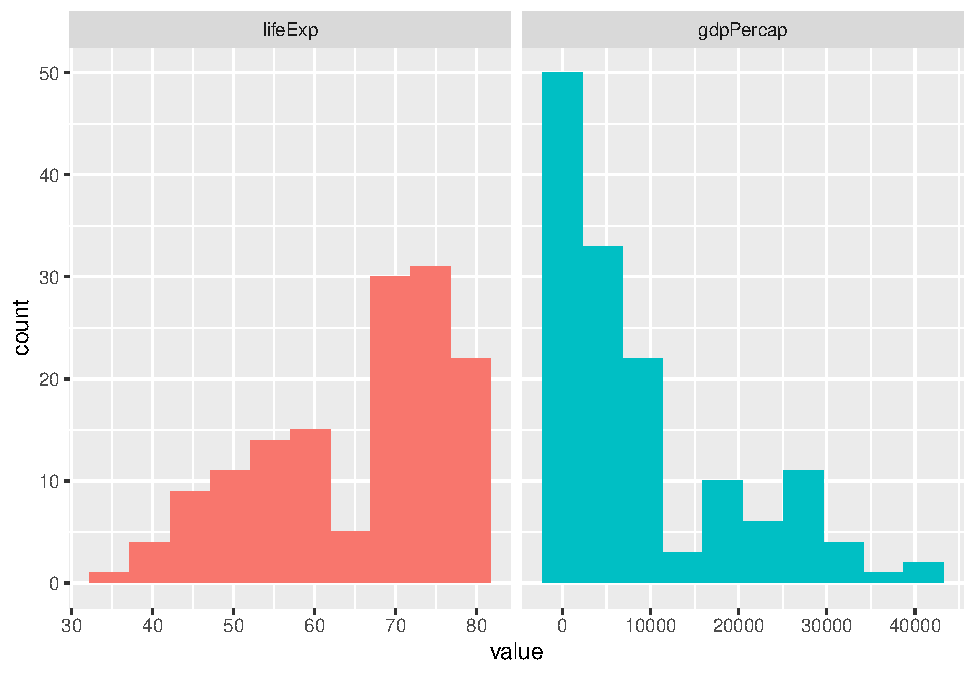
\includegraphics{bookdown-R-Essentials_files/figure-latex/unnamed-chunk-56-1.pdf}

\subsection{Summary Statistics: skimr
package}\label{summary-statistics-skimr-package}

The \emph{skimr} package produces summary statistics about variables and
overviews for dataframes. It is easy to manipulate and use pipes,
select, and filter from the tidyverse family of packages.

The next code supplies a dataframe that contains both categorical
variables (continent), and numeric variables (lifeExp, gdpPercap).
Numeric variables are chosen with the \texttt{yank} function, then some
attributes are omitted from the display (n\_missing, complete\_rate)
using the \texttt{select} function from dplyr.

\begin{Shaded}
\begin{Highlighting}[]
\NormalTok{varlist <-}\StringTok{ }\KeywordTok{c}\NormalTok{(}\StringTok{"n_missing"}\NormalTok{,}\StringTok{"complete_rate"}\NormalTok{)}
\NormalTok{gapminder }\OperatorTok\StringTok{ }\KeywordTok{filter}\NormalTok{(year}\OperatorTok{==}\DecValTok{1997}\NormalTok{) }\OperatorTok\StringTok{ }
\StringTok{  }\KeywordTok{select}\NormalTok{(}\OperatorTok{-}\NormalTok{year, }\OperatorTok{-}\NormalTok{country, }\OperatorTok{-}\NormalTok{pop) }\OperatorTok\StringTok{ }
\StringTok{  }\NormalTok{skimr}\OperatorTok{::}\KeywordTok{skim_without_charts}\NormalTok{() }\OperatorTok
\StringTok{  }\NormalTok{skimr}\OperatorTok{::}\KeywordTok{yank}\NormalTok{(}\StringTok{"numeric"}\NormalTok{) }\OperatorTok
\StringTok{  }\NormalTok{dplyr}\OperatorTok{::}\KeywordTok{select}\NormalTok{(}\OperatorTok{-}\KeywordTok{one_of}\NormalTok{(varlist))}
\end{Highlighting}
\end{Shaded}

\textbf{Variable type: numeric}

\begin{tabular}{l|r|r|r|r|r|r|r}
\hline
skim\_variable & mean & sd & p0 & p25 & p50 & p75 & p100\\
\hline
lifeExp & 65.01 & 11.56 & 36.09 & 55.63 & 69.39 & 74.17 & 80.69\\
\hline
gdpPercap & 9090.18 & 10171.49 & 312.19 & 1366.84 & 4781.83 & 12022.87 & 41283.16\\
\hline
\end{tabular}

\section{One Categorical Variable}\label{one-categorical-variable}

\subsection{Counting Values}\label{counting-values}

The next command counts the number of rows in the dataset for each
continent - then we show a variant which pipes the output into the kable
function for a more attractive table.

\begin{Shaded}
\begin{Highlighting}[]
\NormalTok{gapminder }\OperatorTok\StringTok{ }\KeywordTok{count}\NormalTok{(continent)}
\end{Highlighting}
\end{Shaded}

\begin{verbatim}
## # A tibble: 5 x 2
##   continent     n
##   <fct>     <int>
## 1 Africa      624
## 2 Americas    300
## 3 Asia        396
## 4 Europe      360
## 5 Oceania      24
\end{verbatim}

\begin{Shaded}
\begin{Highlighting}[]
\CommentTok{#}
\NormalTok{gapminder }\OperatorTok\StringTok{  }\KeywordTok{count}\NormalTok{(continent) }\OperatorTok\StringTok{ }\NormalTok{knitr}\OperatorTok{::}\KeywordTok{kable}\NormalTok{()}
\end{Highlighting}
\end{Shaded}

\begin{tabular}{l|r}
\hline
continent & n\\
\hline
Africa & 624\\
\hline
Americas & 300\\
\hline
Asia & 396\\
\hline
Europe & 360\\
\hline
Oceania & 24\\
\hline
\end{tabular}

\begin{Shaded}
\begin{Highlighting}[]
\CommentTok{#}
\NormalTok{gapminder }\OperatorTok\StringTok{  }\KeywordTok{count}\NormalTok{(continent, }\DataTypeTok{sort=}\OtherTok{TRUE}\NormalTok{) }\OperatorTok\StringTok{ }\NormalTok{knitr}\OperatorTok{::}\KeywordTok{kable}\NormalTok{()}
\end{Highlighting}
\end{Shaded}

\begin{tabular}{l|r}
\hline
continent & n\\
\hline
Africa & 624\\
\hline
Asia & 396\\
\hline
Europe & 360\\
\hline
Americas & 300\\
\hline
Oceania & 24\\
\hline
\end{tabular}

The previous code tells us how many lines (rows) for each continent, but
many rows are repeated for each country - just different years.

\begin{Shaded}
\begin{Highlighting}[]
\NormalTok{gapminder }\OperatorTok\StringTok{ }\KeywordTok{filter}\NormalTok{(year}\OperatorTok{==}\DecValTok{1997} \OperatorTok{|}\StringTok{ }\NormalTok{year}\OperatorTok{==}\DecValTok{1967}\NormalTok{) }\OperatorTok
\StringTok{  }\NormalTok{dplyr}\OperatorTok{::}\KeywordTok{group_by}\NormalTok{(continent) }\OperatorTok
\StringTok{  }\NormalTok{dplyr}\OperatorTok{::}\KeywordTok{summarise}\NormalTok{(}\DataTypeTok{n =} \KeywordTok{n}\NormalTok{(), }\DataTypeTok{n_countries =} \KeywordTok{n_distinct}\NormalTok{(country)) }\OperatorTok\StringTok{ }\NormalTok{knitr}\OperatorTok{::}\KeywordTok{kable}\NormalTok{()}
\end{Highlighting}
\end{Shaded}

\begin{tabular}{l|r|r}
\hline
continent & n & n\_countries\\
\hline
Africa & 104 & 52\\
\hline
Americas & 50 & 25\\
\hline
Asia & 66 & 33\\
\hline
Europe & 60 & 30\\
\hline
Oceania & 4 & 2\\
\hline
\end{tabular}

\subsection{Categorical variable: skimr
package}\label{categorical-variable-skimr-package}

Here we summarize a categorical variable (continent), and observe it has
5 unique values (levels) and the most frequent values are displayed.

\begin{Shaded}
\begin{Highlighting}[]
\NormalTok{gapminder }\OperatorTok\StringTok{ }\KeywordTok{filter}\NormalTok{(year}\OperatorTok{==}\DecValTok{1997}\NormalTok{) }\OperatorTok\StringTok{ }
\StringTok{  }\KeywordTok{select}\NormalTok{(lifeExp,continent) }\OperatorTok\StringTok{ }
\StringTok{  }\NormalTok{skimr}\OperatorTok{::}\KeywordTok{skim_without_charts}\NormalTok{() }\OperatorTok
\StringTok{  }\NormalTok{skimr}\OperatorTok{::}\KeywordTok{yank}\NormalTok{(}\StringTok{"factor"}\NormalTok{) }\OperatorTok
\StringTok{  }\NormalTok{dplyr}\OperatorTok{::}\KeywordTok{select}\NormalTok{(}\OperatorTok{-}\NormalTok{n_missing,}\OperatorTok{-}\NormalTok{ordered,}\OperatorTok{-}\NormalTok{complete_rate)}
\end{Highlighting}
\end{Shaded}

\textbf{Variable type: factor}

\begin{tabular}{l|r|l}
\hline
skim\_variable & n\_unique & top\_counts\\
\hline
continent & 5 & Afr: 52, Asi: 33, Eur: 30, Ame: 25\\
\hline
\end{tabular}

\subsection{Categorical variable: funModeling
package}\label{categorical-variable-funmodeling-package}

The \emph{funModeling} package gives an easy way to learn about
categorical variables of types: character and factor. There are two
categorical variables in the gapminder dataframe: country and continent.
There are a lot of countries, so we demonstrate this command for only
the continent variable.

\begin{Shaded}
\begin{Highlighting}[]
\CommentTok{# Frequency distribution of entire dataframe}
\CommentTok{# will produce lots of output and warnings}
\CommentTok{#funModeling::freq(gapminder)}
\CommentTok{# next command for one category variable:  continent}
\NormalTok{funModeling}\OperatorTok{::}\KeywordTok{freq}\NormalTok{(gapminder}\OperatorTok{$}\NormalTok{continent)}
\end{Highlighting}
\end{Shaded}

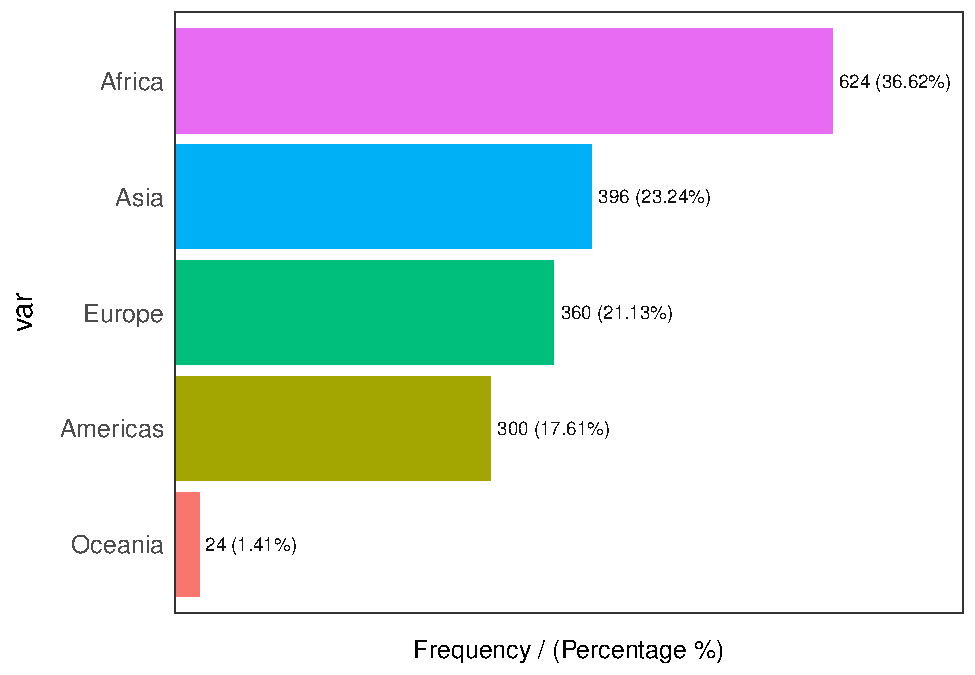
\includegraphics{bookdown-R-Essentials_files/figure-latex/unnamed-chunk-61-1.pdf}

\begin{verbatim}
##        var frequency percentage cumulative_perc
## 1   Africa       624      36.62           36.62
## 2     Asia       396      23.24           59.86
## 3   Europe       360      21.13           80.99
## 4 Americas       300      17.61           98.60
## 5  Oceania        24       1.41          100.00
\end{verbatim}

There are a lot of observations (rows) for Africa and very few for
Oceania (Australia, New Zealand, etc).

\subsection{Categorical variable: janitor
package}\label{categorical-variable-janitor-package}

Let's begin with the base R function \texttt{table}:

\begin{Shaded}
\begin{Highlighting}[]
\NormalTok{gapminder }\OperatorTok\StringTok{ }
\StringTok{  }\KeywordTok{filter}\NormalTok{(year}\OperatorTok{==}\DecValTok{1997}\NormalTok{) }\OperatorTok
\StringTok{  }\KeywordTok{select}\NormalTok{(continent) }\OperatorTok
\StringTok{  }\KeywordTok{table}\NormalTok{()}
\end{Highlighting}
\end{Shaded}

\begin{verbatim}
## .
##   Africa Americas     Asia   Europe  Oceania 
##       52       25       33       30        2
\end{verbatim}

Now contrast with the \texttt{tabyl} function from the \emph{janitor}
package:

\begin{Shaded}
\begin{Highlighting}[]
\NormalTok{gapminder }\OperatorTok\StringTok{ }
\StringTok{  }\KeywordTok{filter}\NormalTok{(year}\OperatorTok{==}\DecValTok{1997}\NormalTok{) }\OperatorTok
\StringTok{  }\NormalTok{janitor}\OperatorTok{::}\KeywordTok{tabyl}\NormalTok{(continent,}\DataTypeTok{sort=}\OtherTok{TRUE}\NormalTok{) }\OperatorTok
\StringTok{  }\NormalTok{knitr}\OperatorTok{::}\KeywordTok{kable}\NormalTok{()}
\end{Highlighting}
\end{Shaded}

\begin{tabular}{l|r|r}
\hline
continent & n & percent\\
\hline
Africa & 52 & 0.3661972\\
\hline
Americas & 25 & 0.1760563\\
\hline
Asia & 33 & 0.2323944\\
\hline
Europe & 30 & 0.2112676\\
\hline
Oceania & 2 & 0.0140845\\
\hline
\end{tabular}

\begin{Shaded}
\begin{Highlighting}[]
\CommentTok{#}
\NormalTok{gapminder }\OperatorTok\StringTok{ }
\StringTok{  }\KeywordTok{filter}\NormalTok{(year}\OperatorTok{==}\DecValTok{1997}\NormalTok{) }\OperatorTok
\StringTok{  }\NormalTok{janitor}\OperatorTok{::}\KeywordTok{tabyl}\NormalTok{(continent,}\DataTypeTok{sort=}\OtherTok{TRUE}\NormalTok{) }\OperatorTok
\StringTok{  }\NormalTok{janitor}\OperatorTok{::}\KeywordTok{adorn_pct_formatting}\NormalTok{(}\DataTypeTok{digits=}\DecValTok{2}\NormalTok{,}\DataTypeTok{affix_sign =} \OtherTok{TRUE}\NormalTok{) }\OperatorTok
\StringTok{  }\NormalTok{knitr}\OperatorTok{::}\KeywordTok{kable}\NormalTok{()}
\end{Highlighting}
\end{Shaded}

\begin{tabular}{l|r|l}
\hline
continent & n & percent\\
\hline
Africa & 52 & 36.62\%\\
\hline
Americas & 25 & 17.61\%\\
\hline
Asia & 33 & 23.24\%\\
\hline
Europe & 30 & 21.13\%\\
\hline
Oceania & 2 & 1.41\%\\
\hline
\end{tabular}

\chapter{Exploratory Data Analysis For One Quantitative Variable: by
Groups}\label{exploratory-data-analysis-for-one-quantitative-variable-by-groups}

It is often helpful to create data summaries of a quantitative variable
for each level of a grouping variable.

\section{Summary Statistics: dplyr}\label{summary-statistics-dplyr}

Using \emph{dplyr} and \emph{tidyverse} for summary statistics across
the levels of a group variable (of type factor/categorical) requires the
use of the verb \texttt{group\_by}. Here we produce summary statistics
of life expectancy across the levels of continent.

\begin{Shaded}
\begin{Highlighting}[]
\CommentTok{# Output presented in initial continent order (alphabetic)}
\NormalTok{gapminder }\OperatorTok\StringTok{ }\KeywordTok{filter}\NormalTok{(year}\OperatorTok{==}\DecValTok{1997}\NormalTok{) }\OperatorTok\StringTok{ }
\StringTok{  }\KeywordTok{filter}\NormalTok{(continent }\OperatorTok{!=}\StringTok{ "Oceania"}\NormalTok{) }\OperatorTok\StringTok{ }
\StringTok{  }\KeywordTok{group_by}\NormalTok{(continent) }\OperatorTok\StringTok{ }
\StringTok{  }\KeywordTok{summarise}\NormalTok{(}\DataTypeTok{meanLE=}\KeywordTok{mean}\NormalTok{(lifeExp,}\DataTypeTok{na.rm=}\OtherTok{TRUE}\NormalTok{),}
            \DataTypeTok{medLE=}\KeywordTok{median}\NormalTok{(lifeExp,}\DataTypeTok{na.rm=}\OtherTok{TRUE}\NormalTok{),}
            \DataTypeTok{sd=}\KeywordTok{sd}\NormalTok{(lifeExp,}\DataTypeTok{na.rm=}\OtherTok{TRUE}\NormalTok{),}
            \DataTypeTok{iqr=}\KeywordTok{IQR}\NormalTok{(lifeExp,}\DataTypeTok{na.rm=}\OtherTok{TRUE}\NormalTok{),}
            \DataTypeTok{Q1=}\KeywordTok{quantile}\NormalTok{(lifeExp, }\DataTypeTok{probs=}\FloatTok{0.25}\NormalTok{,}\DataTypeTok{na.rm=}\OtherTok{TRUE}\NormalTok{),}
            \DataTypeTok{Q3=}\KeywordTok{quantile}\NormalTok{(lifeExp,}\DataTypeTok{probs=}\FloatTok{0.75}\NormalTok{),}
            \DataTypeTok{n=}\KeywordTok{n}\NormalTok{())}
\end{Highlighting}
\end{Shaded}

\begin{verbatim}
## # A tibble: 4 x 8
##   continent meanLE medLE    sd   iqr    Q1    Q3     n
##   <fct>      <dbl> <dbl> <dbl> <dbl> <dbl> <dbl> <int>
## 1 Africa      53.6  52.8  9.10 11.9   47.3  59.2    52
## 2 Americas    71.2  72.1  4.89  4.83  69.4  74.2    25
## 3 Asia        68.0  70.3  8.09 10.7   61.8  72.5    33
## 4 Europe      75.5  76.1  3.10  4.97  73.0  78.0    30
\end{verbatim}

\begin{Shaded}
\begin{Highlighting}[]
\CommentTok{#}
\CommentTok{# Output rows ordered by decreasing values of a statistic (mean Life Expectancy):}
\NormalTok{gapminder }\OperatorTok\StringTok{ }\KeywordTok{filter}\NormalTok{(year}\OperatorTok{==}\DecValTok{1997}\NormalTok{) }\OperatorTok\StringTok{ }
\StringTok{  }\KeywordTok{filter}\NormalTok{(continent }\OperatorTok{!=}\StringTok{ "Oceania"}\NormalTok{) }\OperatorTok\StringTok{ }
\StringTok{  }\KeywordTok{group_by}\NormalTok{(continent) }\OperatorTok
\StringTok{  }\KeywordTok{summarise}\NormalTok{(}\DataTypeTok{meanLE=}\KeywordTok{mean}\NormalTok{(lifeExp,}\DataTypeTok{na.rm=}\OtherTok{TRUE}\NormalTok{),}
            \DataTypeTok{medLE=}\KeywordTok{median}\NormalTok{(lifeExp,}\DataTypeTok{na.rm=}\OtherTok{TRUE}\NormalTok{),}
            \DataTypeTok{sd=}\KeywordTok{sd}\NormalTok{(lifeExp,}\DataTypeTok{na.rm=}\OtherTok{TRUE}\NormalTok{),}
            \DataTypeTok{iqr=}\KeywordTok{IQR}\NormalTok{(lifeExp,}\DataTypeTok{na.rm=}\OtherTok{TRUE}\NormalTok{),}
            \DataTypeTok{min=}\KeywordTok{min}\NormalTok{(lifeExp),}
            \DataTypeTok{max=}\KeywordTok{max}\NormalTok{(lifeExp),}
            \DataTypeTok{n=}\KeywordTok{n}\NormalTok{())  }\OperatorTok
\StringTok{  }\KeywordTok{arrange}\NormalTok{(}\KeywordTok{desc}\NormalTok{(meanLE))}
\end{Highlighting}
\end{Shaded}

\begin{verbatim}
## # A tibble: 4 x 8
##   continent meanLE medLE    sd   iqr   min   max     n
##   <fct>      <dbl> <dbl> <dbl> <dbl> <dbl> <dbl> <int>
## 1 Europe      75.5  76.1  3.10  4.97  68.8  79.4    30
## 2 Americas    71.2  72.1  4.89  4.83  56.7  78.6    25
## 3 Asia        68.0  70.3  8.09 10.7   41.8  80.7    33
## 4 Africa      53.6  52.8  9.10 11.9   36.1  74.8    52
\end{verbatim}

Next, we save the statistics table to an object called statstable, then
we use the \texttt{kable} function for display.

\begin{Shaded}
\begin{Highlighting}[]
\NormalTok{statstable <-}\StringTok{ }\NormalTok{gapminder }\OperatorTok\StringTok{ }\KeywordTok{filter}\NormalTok{(year}\OperatorTok{==}\DecValTok{1997}\NormalTok{) }\OperatorTok\StringTok{ }
\StringTok{  }\KeywordTok{filter}\NormalTok{(continent }\OperatorTok{!=}\StringTok{ "Oceania"}\NormalTok{) }\OperatorTok\StringTok{ }
\StringTok{  }\KeywordTok{group_by}\NormalTok{(continent) }\OperatorTok\StringTok{ }
\StringTok{  }\KeywordTok{summarise}\NormalTok{(}\DataTypeTok{meanLE=}\KeywordTok{mean}\NormalTok{(lifeExp,}\DataTypeTok{na.rm=}\OtherTok{TRUE}\NormalTok{),}
            \DataTypeTok{medLE=}\KeywordTok{median}\NormalTok{(lifeExp,}\DataTypeTok{na.rm=}\OtherTok{TRUE}\NormalTok{),}
            \DataTypeTok{sd=}\KeywordTok{sd}\NormalTok{(lifeExp,}\DataTypeTok{na.rm=}\OtherTok{TRUE}\NormalTok{),}
            \DataTypeTok{iqr=}\KeywordTok{IQR}\NormalTok{(lifeExp,}\DataTypeTok{na.rm=}\OtherTok{TRUE}\NormalTok{),}
            \DataTypeTok{min=}\KeywordTok{min}\NormalTok{(lifeExp),}
            \DataTypeTok{max=}\KeywordTok{max}\NormalTok{(lifeExp),}
            \DataTypeTok{n=}\KeywordTok{n}\NormalTok{())  }\OperatorTok\StringTok{ }
\StringTok{  }\KeywordTok{arrange}\NormalTok{(}\KeywordTok{desc}\NormalTok{(meanLE))}
\CommentTok{#}
\NormalTok{knitr}\OperatorTok{::}\KeywordTok{kable}\NormalTok{(statstable)}
\end{Highlighting}
\end{Shaded}

\begin{tabular}{l|r|r|r|r|r|r|r}
\hline
continent & meanLE & medLE & sd & iqr & min & max & n\\
\hline
Europe & 75.50517 & 76.116 & 3.104677 & 4.96625 & 68.835 & 79.390 & 30\\
\hline
Americas & 71.15048 & 72.146 & 4.887584 & 4.83500 & 56.671 & 78.610 & 25\\
\hline
Asia & 68.02052 & 70.265 & 8.091171 & 10.68100 & 41.763 & 80.690 & 33\\
\hline
Africa & 53.59827 & 52.759 & 9.103387 & 11.92825 & 36.087 & 74.772 & 52\\
\hline
\end{tabular}

\section{Summary Statistics: skimr}\label{summary-statistics-skimr}

Here we implement the \texttt{group\_by} function to display descriptive
statistics for numeric variables by continent, for two quantitative
variables using functions from the \emph{skimr} package.

\begin{Shaded}
\begin{Highlighting}[]
\NormalTok{gapminder }\OperatorTok\StringTok{ }\KeywordTok{filter}\NormalTok{(year}\OperatorTok{==}\DecValTok{1997}\NormalTok{) }\OperatorTok\StringTok{ }
\StringTok{  }\KeywordTok{filter}\NormalTok{(continent }\OperatorTok{!=}\StringTok{ "Oceania"}\NormalTok{) }\OperatorTok\StringTok{ }
\StringTok{  }\KeywordTok{group_by}\NormalTok{(continent) }\OperatorTok\StringTok{ }
\StringTok{  }\NormalTok{skimr}\OperatorTok{::}\KeywordTok{skim_without_charts}\NormalTok{() }\OperatorTok
\StringTok{  }\NormalTok{skimr}\OperatorTok{::}\KeywordTok{yank}\NormalTok{(}\StringTok{"numeric"}\NormalTok{) }\OperatorTok
\StringTok{  }\NormalTok{dplyr}\OperatorTok{::}\KeywordTok{filter}\NormalTok{(skim_variable }\OperatorTok\StringTok{ }\KeywordTok{c}\NormalTok{(}\StringTok{"lifeExp"}\NormalTok{,}\StringTok{"gdpPercap"}\NormalTok{)) }\OperatorTok
\StringTok{  }\NormalTok{knitr}\OperatorTok{::}\KeywordTok{kable}\NormalTok{()}
\end{Highlighting}
\end{Shaded}

\begin{tabular}{l|l|r|r|r|r|r|r|r|r|r}
\hline
skim\_variable & continent & n\_missing & complete\_rate & mean & sd & p0 & p25 & p50 & p75 & p100\\
\hline
lifeExp & Africa & 0 & 1 & 53.59827 & 9.103387 & 36.0870 & 47.30025 & 52.759 & 59.22850 & 74.772\\
\hline
lifeExp & Americas & 0 & 1 & 71.15048 & 4.887584 & 56.6710 & 69.38800 & 72.146 & 74.22300 & 78.610\\
\hline
lifeExp & Asia & 0 & 1 & 68.02052 & 8.091171 & 41.7630 & 61.81800 & 70.265 & 72.49900 & 80.690\\
\hline
lifeExp & Europe & 0 & 1 & 75.50517 & 3.104677 & 68.8350 & 73.02350 & 76.116 & 77.98975 & 79.390\\
\hline
gdpPercap & Africa & 0 & 1 & 2378.75956 & 2820.728117 & 312.1884 & 791.90197 & 1179.883 & 2856.38603 & 14722.842\\
\hline
gdpPercap & Americas & 0 & 1 & 8889.30086 & 7874.225145 & 1341.7269 & 4684.31381 & 7113.692 & 9767.29753 & 35767.433\\
\hline
gdpPercap & Asia & 0 & 1 & 9834.09330 & 11094.180481 & 415.0000 & 1902.25210 & 3645.380 & 19702.05581 & 40300.620\\
\hline
gdpPercap & Europe & 0 & 1 & 19076.78180 & 10065.457716 & 3193.0546 & 9946.59931 & 19596.499 & 27189.53031 & 41283.164\\
\hline
\end{tabular}

\section{Graphical Displays of a quantitative variable, separated by
groups}\label{graphical-displays-of-a-quantitative-variable-separated-by-groups}

In each example, the first lines create the dataset to be graphed -
followed by a \texttt{ggplot} command making the display. Several of the
examples make use of the principle of ``small-multiples'' so that each
level of the factor variable has a separarate panel for the quantitative
variable display.

\subsection{Dotplots}\label{dotplots}

\begin{Shaded}
\begin{Highlighting}[]
\NormalTok{ds <-}\StringTok{ }\NormalTok{gapminder }\OperatorTok\StringTok{ }\KeywordTok{filter}\NormalTok{(year}\OperatorTok{==}\DecValTok{1997}\NormalTok{) }
\CommentTok{#}
\KeywordTok{ggplot}\NormalTok{(}\DataTypeTok{data=}\NormalTok{ds,}\DataTypeTok{mapping=}\KeywordTok{aes}\NormalTok{(}\DataTypeTok{x=}\NormalTok{lifeExp)) }\OperatorTok{+}\StringTok{ }
\StringTok{  }\KeywordTok{geom_dotplot}\NormalTok{() }\OperatorTok{+}\StringTok{ }
\StringTok{  }\KeywordTok{facet_wrap}\NormalTok{( }\OperatorTok{~}\StringTok{ }\NormalTok{continent,}\DataTypeTok{ncol=}\DecValTok{2}\NormalTok{) }\OperatorTok{+}\StringTok{ }
\StringTok{  }\KeywordTok{xlab}\NormalTok{(}\StringTok{"Life Expectancy (years)"}\NormalTok{) }\OperatorTok{+}
\StringTok{  }\KeywordTok{ylab}\NormalTok{(}\StringTok{"Frequency"}\NormalTok{)}
\end{Highlighting}
\end{Shaded}

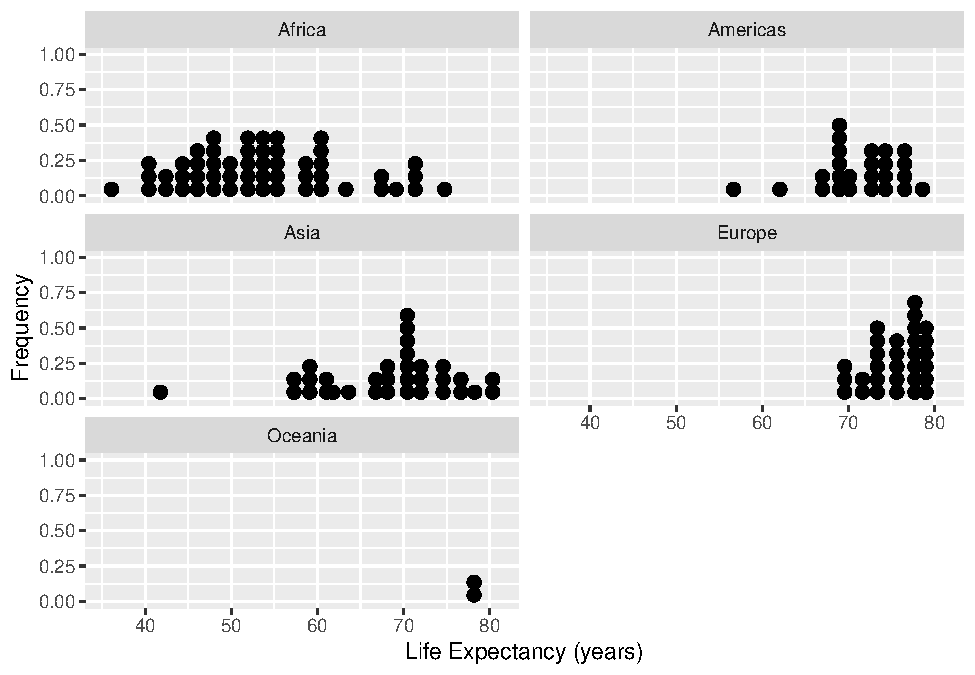
\includegraphics{bookdown-R-Essentials_files/figure-latex/unnamed-chunk-68-1.pdf}

\subsection{Histograms}\label{histograms}

\begin{Shaded}
\begin{Highlighting}[]
\NormalTok{ds <-}\StringTok{ }\NormalTok{gapminder }\OperatorTok\StringTok{ }
\StringTok{  }\KeywordTok{filter}\NormalTok{(year}\OperatorTok{==}\DecValTok{1997}\NormalTok{) }\OperatorTok\StringTok{ }
\StringTok{  }\KeywordTok{filter}\NormalTok{(continent }\OperatorTok{!=}\StringTok{ "Oceania"}\NormalTok{) }\OperatorTok\StringTok{ }
\StringTok{  }\KeywordTok{group_by}\NormalTok{(continent) }
\CommentTok{#}
\KeywordTok{ggplot}\NormalTok{(}\DataTypeTok{data=}\NormalTok{ds, }\DataTypeTok{mapping=}\KeywordTok{aes}\NormalTok{(}\DataTypeTok{x=}\NormalTok{lifeExp)) }\OperatorTok{+}\StringTok{ }
\StringTok{  }\KeywordTok{geom_histogram}\NormalTok{(}\DataTypeTok{binwidth=}\DecValTok{5}\NormalTok{) }\OperatorTok{+}\StringTok{ }
\StringTok{  }\KeywordTok{facet_wrap}\NormalTok{( }\OperatorTok{~}\StringTok{ }\NormalTok{continent,}\DataTypeTok{ncol=}\DecValTok{2}\NormalTok{) }\OperatorTok{+}\StringTok{ }
\StringTok{  }\KeywordTok{xlab}\NormalTok{(}\StringTok{"Life Expectancy (years)"}\NormalTok{) }\OperatorTok{+}
\StringTok{  }\KeywordTok{ylab}\NormalTok{(}\StringTok{"Frequency"}\NormalTok{)}
\end{Highlighting}
\end{Shaded}

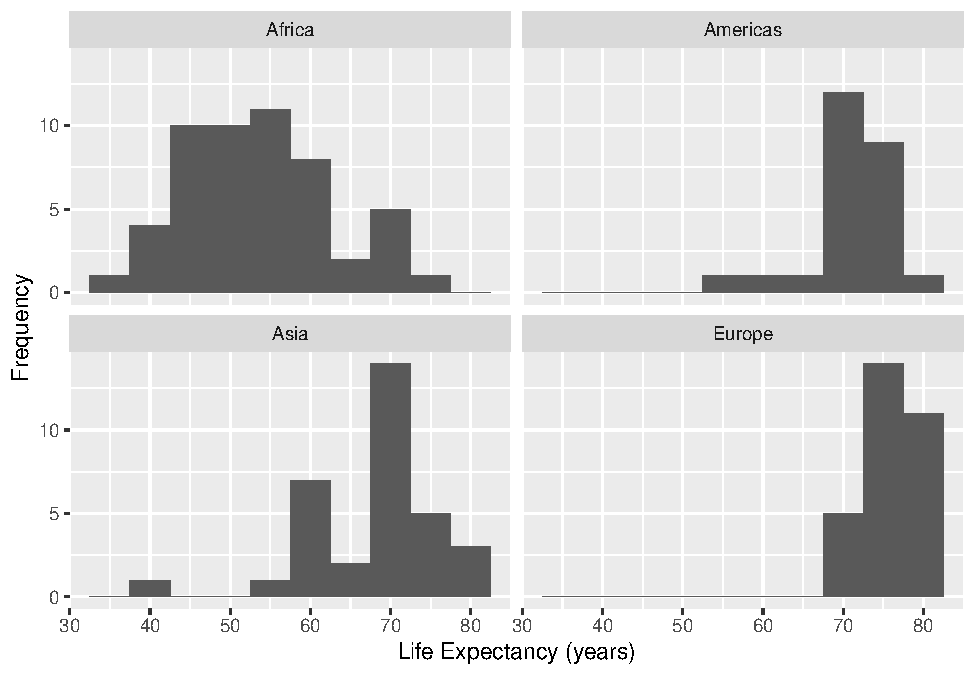
\includegraphics{bookdown-R-Essentials_files/figure-latex/unnamed-chunk-69-1.pdf}

\subsection{Density Plots in Facets}\label{density-plots-in-facets}

The code given here shows how to produce a density plot in separate
panels for each continent.

\begin{Shaded}
\begin{Highlighting}[]
\NormalTok{ds <-}\StringTok{ }\NormalTok{gapminder }\OperatorTok\StringTok{ }
\StringTok{  }\KeywordTok{filter}\NormalTok{(year}\OperatorTok{==}\DecValTok{1997}\NormalTok{) }\OperatorTok\StringTok{ }
\StringTok{  }\KeywordTok{filter}\NormalTok{(continent }\OperatorTok{!=}\StringTok{ "Oceania"}\NormalTok{) }\OperatorTok\StringTok{ }
\StringTok{  }\KeywordTok{group_by}\NormalTok{(continent) }
\CommentTok{#}
\KeywordTok{ggplot}\NormalTok{(}\DataTypeTok{data=}\NormalTok{ds, }\DataTypeTok{mapping=}\KeywordTok{aes}\NormalTok{(}\DataTypeTok{x=}\NormalTok{lifeExp, }\DataTypeTok{colour=}\NormalTok{continent, }\DataTypeTok{fill=}\NormalTok{continent)) }\OperatorTok{+}\StringTok{ }
\StringTok{  }\KeywordTok{geom_density}\NormalTok{(}\DataTypeTok{alpha =} \FloatTok{0.35}\NormalTok{) }\OperatorTok{+}\StringTok{ }
\StringTok{  }\KeywordTok{xlab}\NormalTok{(}\StringTok{"Life Expectancy (years)"}\NormalTok{) }\OperatorTok{+}
\StringTok{  }\KeywordTok{ylab}\NormalTok{(}\StringTok{"Density"}\NormalTok{) }\OperatorTok{+}
\StringTok{  }\KeywordTok{facet_wrap}\NormalTok{( }\OperatorTok{~}\StringTok{ }\NormalTok{continent, }\DataTypeTok{ncol =} \DecValTok{2}\NormalTok{) }\OperatorTok{+}\StringTok{  }
\StringTok{  }\KeywordTok{theme}\NormalTok{(}\DataTypeTok{legend.position =} \StringTok{"none"}\NormalTok{)}
\end{Highlighting}
\end{Shaded}

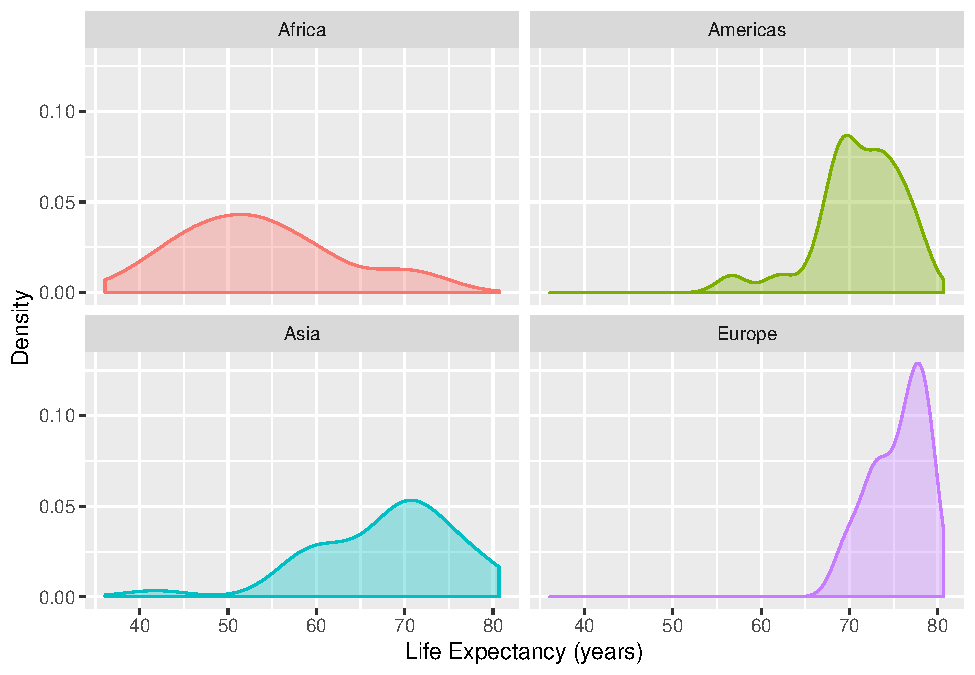
\includegraphics{bookdown-R-Essentials_files/figure-latex/unnamed-chunk-70-1.pdf}

\subsection{Overlaid Density Plots}\label{overlaid-density-plots}

The initial command below takes the gapminder data and consider only
observations (rows) from 1997, but exclude all observations from
Oceania. The \texttt{alpha} setting controls the amount of transparency
in the densities for each continent - smaller values of \texttt{alpha}
(between 0 and 1) are more transparent.

\begin{Shaded}
\begin{Highlighting}[]
\NormalTok{gapminder }\OperatorTok\StringTok{ }
\StringTok{  }\KeywordTok{filter}\NormalTok{(year}\OperatorTok{==}\DecValTok{1997}\NormalTok{) }\OperatorTok\StringTok{ }
\StringTok{  }\KeywordTok{filter}\NormalTok{(continent }\OperatorTok{!=}\StringTok{ "Oceania"}\NormalTok{) }\OperatorTok\StringTok{ }
\StringTok{  }\KeywordTok{group_by}\NormalTok{(continent) }\OperatorTok
\KeywordTok{ggplot}\NormalTok{(}\DataTypeTok{mapping=}\KeywordTok{aes}\NormalTok{(}\DataTypeTok{x=}\NormalTok{lifeExp, }\DataTypeTok{colour=}\NormalTok{continent, }\DataTypeTok{fill=}\NormalTok{continent)) }\OperatorTok{+}\StringTok{ }
\StringTok{  }\KeywordTok{geom_density}\NormalTok{(}\DataTypeTok{alpha =} \FloatTok{0.35}\NormalTok{) }\OperatorTok{+}\StringTok{ }
\StringTok{  }\KeywordTok{xlab}\NormalTok{(}\StringTok{"Life Expectancy (years)"}\NormalTok{) }\OperatorTok{+}
\StringTok{  }\KeywordTok{ylab}\NormalTok{(}\StringTok{"Density"}\NormalTok{)}
\end{Highlighting}
\end{Shaded}

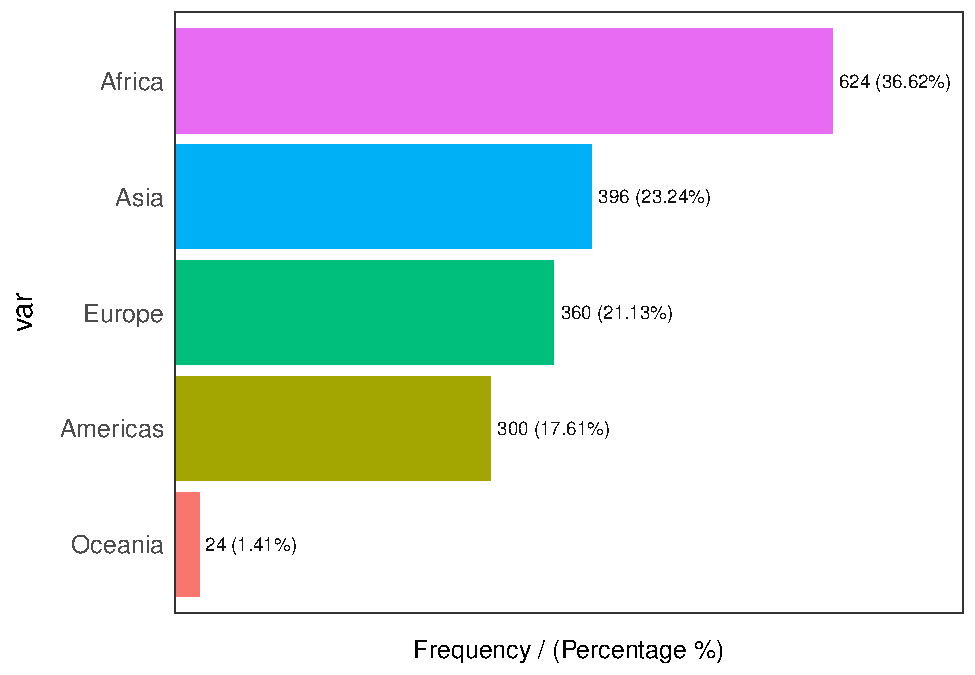
\includegraphics{bookdown-R-Essentials_files/figure-latex/unnamed-chunk-71-1.pdf}

\subsection{Boxplots, Grouped Data}\label{boxplots-grouped-data}

In the code below, the \texttt{alpha} value again controls the
transparency of the points alpha=1 means opaque, alpha=0 means
completely see-through. When there is a lot of data, use a smaller value
of alpha.

\begin{Shaded}
\begin{Highlighting}[]
\NormalTok{ds <-}\StringTok{ }\NormalTok{gapminder }\OperatorTok\StringTok{ }
\StringTok{  }\KeywordTok{filter}\NormalTok{(year}\OperatorTok{==}\DecValTok{1997}\NormalTok{) }\OperatorTok\StringTok{ }
\StringTok{  }\KeywordTok{filter}\NormalTok{(continent }\OperatorTok{!=}\StringTok{ "Oceania"}\NormalTok{) }\OperatorTok\StringTok{ }
\StringTok{  }\KeywordTok{group_by}\NormalTok{(continent) }
\CommentTok{#}
\KeywordTok{ggplot}\NormalTok{(}\DataTypeTok{data=}\NormalTok{ds, }\DataTypeTok{mapping=}\KeywordTok{aes}\NormalTok{(}\DataTypeTok{x=}\NormalTok{continent,}\DataTypeTok{y=}\NormalTok{lifeExp)) }\OperatorTok{+}
\StringTok{ }\KeywordTok{geom_boxplot}\NormalTok{() }\OperatorTok{+}\StringTok{ }
\StringTok{  }\KeywordTok{labs}\NormalTok{(}\DataTypeTok{x=}\StringTok{"Continent"}\NormalTok{,}\DataTypeTok{y=}\StringTok{"Life Expectancy (years)"}\NormalTok{)}
\end{Highlighting}
\end{Shaded}

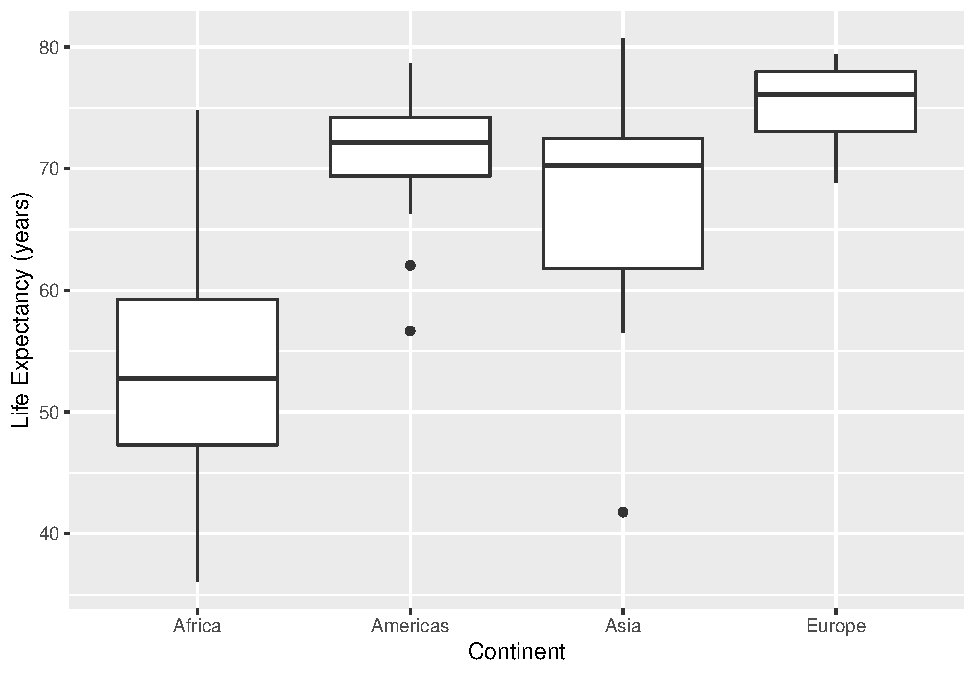
\includegraphics{bookdown-R-Essentials_files/figure-latex/unnamed-chunk-72-1.pdf}

\begin{Shaded}
\begin{Highlighting}[]
\CommentTok{#}
\KeywordTok{ggplot}\NormalTok{(}\DataTypeTok{data=}\NormalTok{ds, }\DataTypeTok{mapping=}\KeywordTok{aes}\NormalTok{(}\DataTypeTok{x=}\NormalTok{continent,}\DataTypeTok{y=}\NormalTok{lifeExp)) }\OperatorTok{+}\StringTok{  }
\StringTok{ }\KeywordTok{geom_boxplot}\NormalTok{(}\DataTypeTok{outlier.colour =} \OtherTok{NA}\NormalTok{) }\OperatorTok{+}\StringTok{ }
\StringTok{ }\KeywordTok{geom_point}\NormalTok{(}\DataTypeTok{position =} \KeywordTok{position_jitter}\NormalTok{(}\DataTypeTok{width =} \FloatTok{0.15}\NormalTok{, }\DataTypeTok{height =} \FloatTok{0.15}\NormalTok{),}\DataTypeTok{alpha=}\NormalTok{.}\DecValTok{50}\NormalTok{) }\OperatorTok{+}
\StringTok{  }\KeywordTok{labs}\NormalTok{(}\DataTypeTok{x=}\StringTok{"Continent"}\NormalTok{,}\DataTypeTok{y=}\StringTok{"Life Expectancy (years)"}\NormalTok{)}
\end{Highlighting}
\end{Shaded}

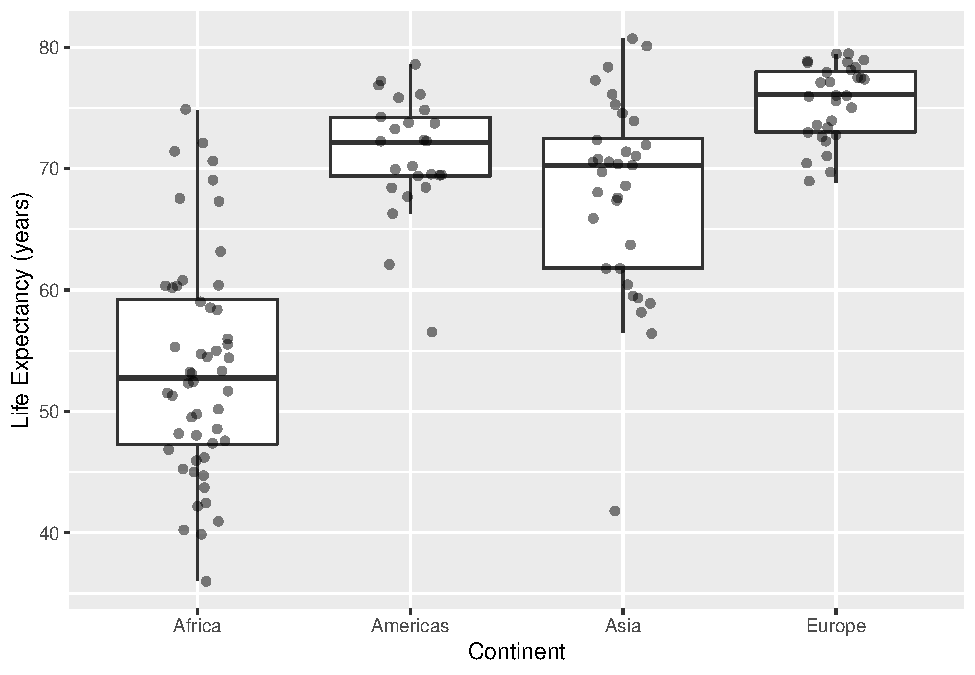
\includegraphics{bookdown-R-Essentials_files/figure-latex/unnamed-chunk-72-2.pdf}

\subsection{Boxplots, overlay points on the boxplots with color
control}\label{boxplots-overlay-points-on-the-boxplots-with-color-control}

In the code below, the alpha value controls the transparency of the
points alpha=1 means opaque, alpha=0 means completely see-through.

\begin{Shaded}
\begin{Highlighting}[]
\NormalTok{ds <-}\StringTok{ }\NormalTok{gapminder }\OperatorTok\StringTok{ }
\StringTok{  }\KeywordTok{filter}\NormalTok{(year}\OperatorTok{==}\DecValTok{1997}\NormalTok{) }\OperatorTok\StringTok{ }
\StringTok{  }\KeywordTok{filter}\NormalTok{(continent }\OperatorTok{!=}\StringTok{ "Oceania"}\NormalTok{) }\OperatorTok\StringTok{ }
\StringTok{  }\KeywordTok{group_by}\NormalTok{(continent) }
\CommentTok{# }
\KeywordTok{ggplot}\NormalTok{(}\DataTypeTok{data=}\NormalTok{ds, }\DataTypeTok{mapping=}\KeywordTok{aes}\NormalTok{(}\DataTypeTok{x=}\NormalTok{continent,}\DataTypeTok{y=}\NormalTok{lifeExp, }\DataTypeTok{colour=}\NormalTok{continent)) }\OperatorTok{+}\StringTok{ }
\StringTok{  }\KeywordTok{geom_point}\NormalTok{(}\DataTypeTok{position =} \KeywordTok{position_jitter}\NormalTok{(}\DataTypeTok{width =} \FloatTok{0.2}\NormalTok{, }\DataTypeTok{height =} \FloatTok{0.2}\NormalTok{),}\DataTypeTok{alpha=}\NormalTok{.}\DecValTok{25}\NormalTok{) }\OperatorTok{+}
\StringTok{ }\KeywordTok{geom_boxplot}\NormalTok{(}\DataTypeTok{outlier.colour =} \OtherTok{NA}\NormalTok{, }\DataTypeTok{fill =} \OtherTok{NA}\NormalTok{) }\OperatorTok{+}\StringTok{ }
\StringTok{  }\KeywordTok{labs}\NormalTok{(}\DataTypeTok{x=}\StringTok{"Continent"}\NormalTok{,}\DataTypeTok{y=}\StringTok{"Life Expectancy (years)"}\NormalTok{)}
\end{Highlighting}
\end{Shaded}

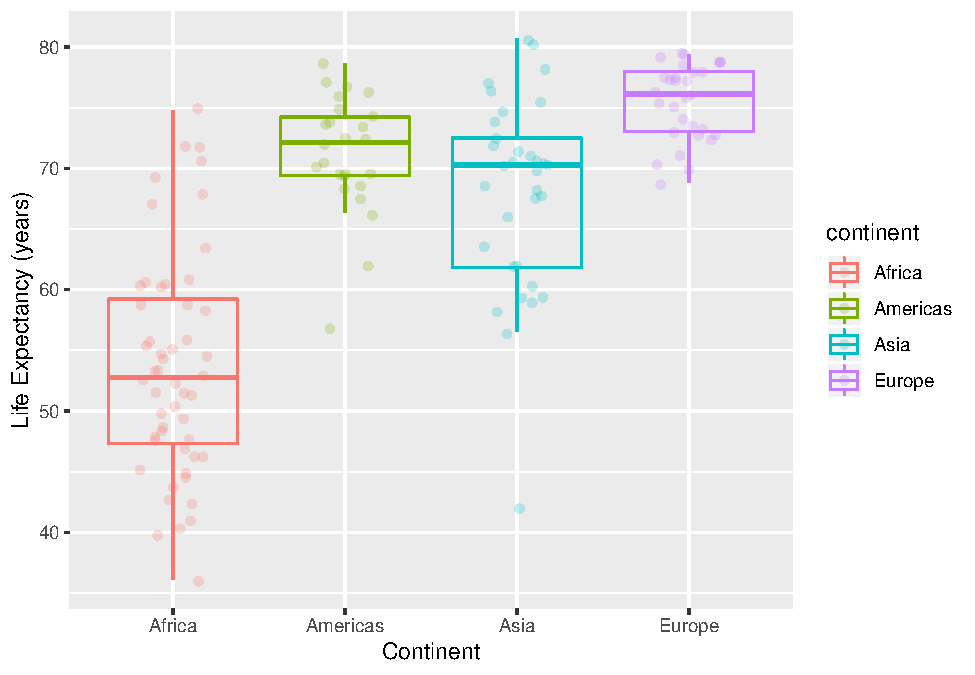
\includegraphics{bookdown-R-Essentials_files/figure-latex/oztempbox2-1.pdf}

\begin{Shaded}
\begin{Highlighting}[]
\CommentTok{# }
\KeywordTok{ggplot}\NormalTok{(}\DataTypeTok{data=}\NormalTok{ds, }\DataTypeTok{mapping=}\KeywordTok{aes}\NormalTok{(}\DataTypeTok{x=}\NormalTok{continent,}\DataTypeTok{y=}\NormalTok{lifeExp, }\DataTypeTok{colour=}\NormalTok{continent)) }\OperatorTok{+}\StringTok{ }
\StringTok{  }\KeywordTok{geom_point}\NormalTok{(}\DataTypeTok{position =} \KeywordTok{position_jitter}\NormalTok{(}\DataTypeTok{width =} \FloatTok{0.2}\NormalTok{, }\DataTypeTok{height =} \FloatTok{0.2}\NormalTok{),}\DataTypeTok{alpha=}\NormalTok{.}\DecValTok{80}\NormalTok{) }\OperatorTok{+}
\StringTok{ }\KeywordTok{geom_boxplot}\NormalTok{(}\DataTypeTok{outlier.colour =} \OtherTok{NA}\NormalTok{, }\DataTypeTok{fill =} \OtherTok{NA}\NormalTok{) }\OperatorTok{+}\StringTok{ }
\StringTok{  }\KeywordTok{labs}\NormalTok{(}\DataTypeTok{x=}\StringTok{"Continent"}\NormalTok{,}\DataTypeTok{y=}\StringTok{"Life Expectancy (years)"}\NormalTok{)}
\end{Highlighting}
\end{Shaded}

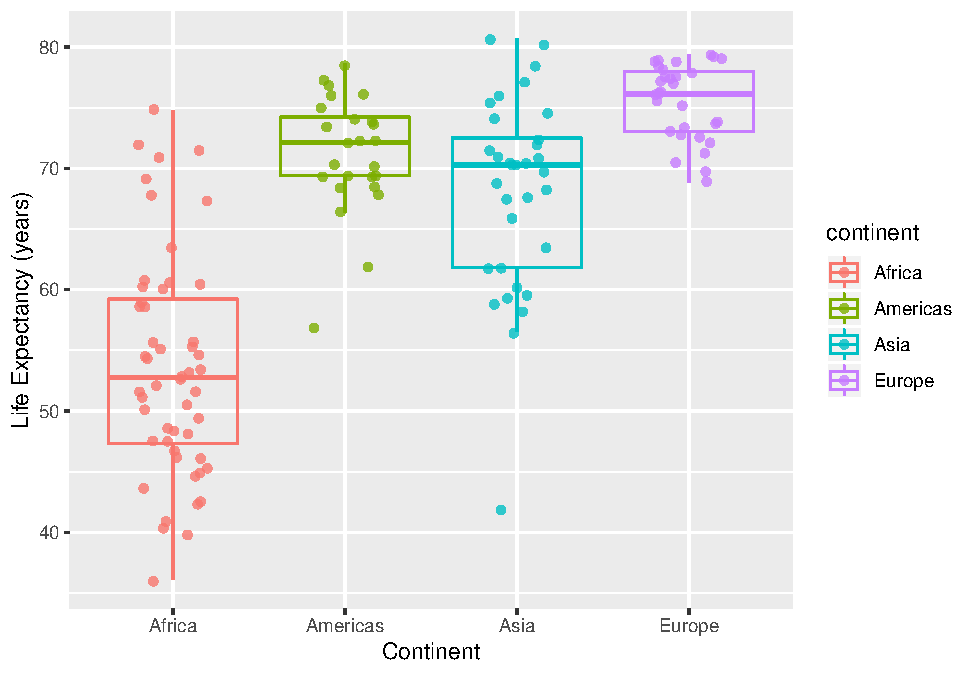
\includegraphics{bookdown-R-Essentials_files/figure-latex/oztempbox2-2.pdf}

\chapter{Analysis of One Categorical Variable by another categorical
variable}\label{analysis-of-one-categorical-variable-by-another-categorical-variable}

To demonstrate graphical displays of two categorical variables, we need
a new dataset with two categorical variables. We use the
\texttt{congress\_age} dataframe from the \emph{fivethirtyeight}
package. In these displays we will use categorical variables:

\begin{itemize}
\tightlist
\item
  party affiliation (party) with values: D, I, R.
\item
  congressional chamber (chamber) with values: house, senate
\end{itemize}

We will restrict ourselves to the 113th congress, a meeting of the
legislative branch of the United States federal government, from January
3, 2013, to January 3, 2015, during the fifth and sixth years of Barack
Obama's presidency.

\section{Tables}\label{tables}

\begin{Shaded}
\begin{Highlighting}[]
\NormalTok{congage <-}\StringTok{ }\NormalTok{fivethirtyeight}\OperatorTok{::}\NormalTok{congress_age}
\NormalTok{ds1 <-}\StringTok{ }\NormalTok{congage }\OperatorTok\StringTok{ }\KeywordTok{filter}\NormalTok{(congress }\OperatorTok{>}\StringTok{ }\DecValTok{112}\NormalTok{) }\OperatorTok\StringTok{ }\KeywordTok{select}\NormalTok{(congress,chamber,state,party,incumbent,age) }
\CommentTok{#  We declare party and chamber as factor/categorical variables, and control their levels.}
\NormalTok{ds1 <-}\StringTok{ }\NormalTok{ds1 }\OperatorTok\StringTok{ }\KeywordTok{mutate}\NormalTok{(}\DataTypeTok{party =} \KeywordTok{factor}\NormalTok{(party,}\DataTypeTok{levels=}\KeywordTok{c}\NormalTok{(}\StringTok{"D"}\NormalTok{,}\StringTok{"I"}\NormalTok{,}\StringTok{"R"}\NormalTok{)),}
                    \DataTypeTok{chamber =} \KeywordTok{factor}\NormalTok{(chamber))}
\NormalTok{ds1 <-}\StringTok{ }\NormalTok{ds1 }\OperatorTok\StringTok{ }\KeywordTok{na.omit}\NormalTok{()}
\NormalTok{ds <-}\StringTok{ }\NormalTok{ds1  }
\CommentTok{#}
\KeywordTok{table}\NormalTok{(ds}\OperatorTok{$}\NormalTok{chamber,ds}\OperatorTok{$}\NormalTok{party)}
\end{Highlighting}
\end{Shaded}

\begin{verbatim}
##         
##            D   I   R
##   house  202   0 237
##   senate  57   2  46
\end{verbatim}

\begin{Shaded}
\begin{Highlighting}[]
\CommentTok{#}
\NormalTok{mytable <-}\StringTok{ }\KeywordTok{table}\NormalTok{(ds}\OperatorTok{$}\NormalTok{chamber,ds}\OperatorTok{$}\NormalTok{party)}
\CommentTok{#}
\KeywordTok{prop.table}\NormalTok{(mytable) }\CommentTok{# cell percentages}
\end{Highlighting}
\end{Shaded}

\begin{verbatim}
##         
##                    D           I           R
##   house  0.371323529 0.000000000 0.435661765
##   senate 0.104779412 0.003676471 0.084558824
\end{verbatim}

\begin{Shaded}
\begin{Highlighting}[]
\KeywordTok{prop.table}\NormalTok{(mytable, }\DecValTok{1}\NormalTok{) }\CommentTok{# row percentages}
\end{Highlighting}
\end{Shaded}

\begin{verbatim}
##         
##                   D          I          R
##   house  0.46013667 0.00000000 0.53986333
##   senate 0.54285714 0.01904762 0.43809524
\end{verbatim}

\begin{Shaded}
\begin{Highlighting}[]
\KeywordTok{prop.table}\NormalTok{(mytable, }\DecValTok{2}\NormalTok{) }\CommentTok{# column percentages}
\end{Highlighting}
\end{Shaded}

\begin{verbatim}
##         
##                  D         I         R
##   house  0.7799228 0.0000000 0.8374558
##   senate 0.2200772 1.0000000 0.1625442
\end{verbatim}

\begin{Shaded}
\begin{Highlighting}[]
\NormalTok{ds }\OperatorTok\StringTok{  }\NormalTok{janitor}\OperatorTok{::}\KeywordTok{tabyl}\NormalTok{(chamber, party)}
\end{Highlighting}
\end{Shaded}

\begin{verbatim}
##  chamber   D I   R
##    house 202 0 237
##   senate  57 2  46
\end{verbatim}

\begin{Shaded}
\begin{Highlighting}[]
\CommentTok{#}
\NormalTok{t2 <-}\StringTok{ }\NormalTok{ds }\OperatorTok\StringTok{  }\NormalTok{janitor}\OperatorTok{::}\KeywordTok{tabyl}\NormalTok{(chamber, party)}
\NormalTok{t2 }\OperatorTok
\StringTok{  }\NormalTok{janitor}\OperatorTok{::}\KeywordTok{adorn_percentages}\NormalTok{(}\StringTok{"row"}\NormalTok{) }\OperatorTok
\StringTok{  }\NormalTok{janitor}\OperatorTok{::}\KeywordTok{adorn_pct_formatting}\NormalTok{(}\DataTypeTok{digits =} \DecValTok{2}\NormalTok{) }\OperatorTok
\StringTok{  }\NormalTok{janitor}\OperatorTok{::}\KeywordTok{adorn_ns}\NormalTok{()}
\end{Highlighting}
\end{Shaded}

\begin{verbatim}
##  chamber            D         I            R
##    house 46.01% (202) 0.00% (0) 53.99% (237)
##   senate 54.29%  (57) 1.90% (2) 43.81%  (46)
\end{verbatim}

\begin{Shaded}
\begin{Highlighting}[]
\CommentTok{# column percentages}
\NormalTok{t2 }\OperatorTok
\StringTok{  }\NormalTok{janitor}\OperatorTok{::}\KeywordTok{adorn_percentages}\NormalTok{(}\StringTok{"col"}\NormalTok{) }\OperatorTok
\StringTok{  }\NormalTok{janitor}\OperatorTok{::}\KeywordTok{adorn_pct_formatting}\NormalTok{(}\DataTypeTok{digits =} \DecValTok{2}\NormalTok{) }\OperatorTok
\StringTok{  }\NormalTok{janitor}\OperatorTok{::}\KeywordTok{adorn_ns}\NormalTok{()}
\end{Highlighting}
\end{Shaded}

\begin{verbatim}
##  chamber            D           I            R
##    house 77.99% (202)   0.00% (0) 83.75% (237)
##   senate 22.01%  (57) 100.00% (2) 16.25%  (46)
\end{verbatim}

\begin{Shaded}
\begin{Highlighting}[]
\CommentTok{# both row and column percentages}
\NormalTok{t2 }\OperatorTok
\StringTok{  }\NormalTok{janitor}\OperatorTok{::}\KeywordTok{adorn_percentages}\NormalTok{(}\StringTok{"all"}\NormalTok{) }\OperatorTok
\StringTok{  }\NormalTok{janitor}\OperatorTok{::}\KeywordTok{adorn_pct_formatting}\NormalTok{(}\DataTypeTok{digits =} \DecValTok{2}\NormalTok{) }\OperatorTok
\StringTok{  }\NormalTok{janitor}\OperatorTok{::}\KeywordTok{adorn_ns}\NormalTok{()}
\end{Highlighting}
\end{Shaded}

\begin{verbatim}
##  chamber            D         I            R
##    house 37.13% (202) 0.00% (0) 43.57% (237)
##   senate 10.48%  (57) 0.37% (2)  8.46%  (46)
\end{verbatim}

\begin{Shaded}
\begin{Highlighting}[]
\NormalTok{congage <-}\StringTok{ }\NormalTok{fivethirtyeight}\OperatorTok{::}\NormalTok{congress_age}
\NormalTok{ds1 <-}\StringTok{ }\NormalTok{congage }\OperatorTok\StringTok{ }\KeywordTok{filter}\NormalTok{(congress }\OperatorTok{>}\StringTok{ }\DecValTok{112}\NormalTok{) }\OperatorTok\StringTok{ }\KeywordTok{select}\NormalTok{(congress,chamber,state,party,incumbent,age) }
\CommentTok{#  We declare party and chamber as factor/categorical variables, and control their levels.}
\NormalTok{ds1 <-}\StringTok{ }\NormalTok{ds1 }\OperatorTok\StringTok{ }\KeywordTok{mutate}\NormalTok{(}\DataTypeTok{party =} \KeywordTok{factor}\NormalTok{(party,}\DataTypeTok{levels=}\KeywordTok{c}\NormalTok{(}\StringTok{"D"}\NormalTok{,}\StringTok{"I"}\NormalTok{,}\StringTok{"R"}\NormalTok{)),}
                    \DataTypeTok{chamber =} \KeywordTok{factor}\NormalTok{(chamber))}
\NormalTok{ds1 <-}\StringTok{ }\NormalTok{ds1 }\OperatorTok\StringTok{ }\KeywordTok{na.omit}\NormalTok{()}
\NormalTok{ds <-}\StringTok{ }\NormalTok{ds1  }
\NormalTok{ds }\OperatorTok\StringTok{ }\KeywordTok{group_by}\NormalTok{(chamber,party) }\OperatorTok\StringTok{ }
\StringTok{  }\NormalTok{dplyr}\OperatorTok{::}\KeywordTok{count}\NormalTok{() }\OperatorTok\StringTok{ }
\StringTok{  }\NormalTok{tidyr}\OperatorTok{::}\KeywordTok{pivot_wider}\NormalTok{(}\DataTypeTok{names_from =}\NormalTok{ party, }\DataTypeTok{values_from =}\NormalTok{ n)}
\end{Highlighting}
\end{Shaded}

\begin{verbatim}
## # A tibble: 2 x 4
## # Groups:   chamber [2]
##   chamber     D     R     I
##   <fct>   <int> <int> <int>
## 1 house     202   237    NA
## 2 senate     57    46     2
\end{verbatim}

\section{Graphical Displays}\label{graphical-displays}

\begin{Shaded}
\begin{Highlighting}[]
\CommentTok{# basic bar plot of party affiliation}
\KeywordTok{ggplot}\NormalTok{(}\DataTypeTok{data=}\NormalTok{ds, }\KeywordTok{aes}\NormalTok{(}\DataTypeTok{x=}\NormalTok{party)) }\OperatorTok{+}\StringTok{ }\KeywordTok{geom_bar}\NormalTok{() }\OperatorTok{+}
\StringTok{  }\KeywordTok{labs}\NormalTok{(}\DataTypeTok{x=}\StringTok{"Party"}\NormalTok{, }\DataTypeTok{y=}\StringTok{"Count"}\NormalTok{)}
\end{Highlighting}
\end{Shaded}

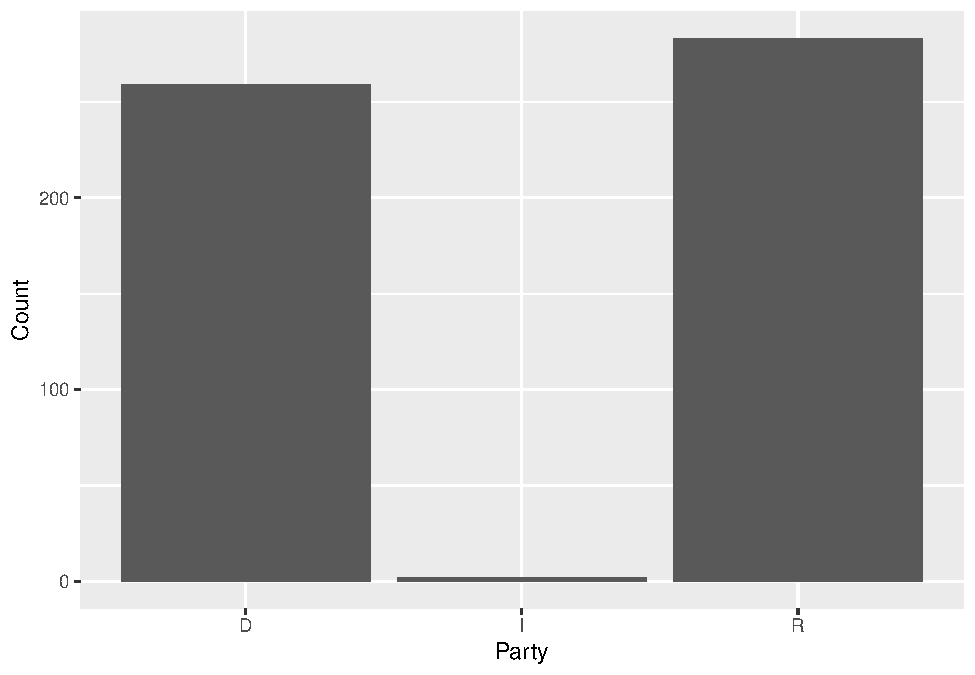
\includegraphics{bookdown-R-Essentials_files/figure-latex/unnamed-chunk-77-1.pdf}

\begin{Shaded}
\begin{Highlighting}[]
\NormalTok{ds <-}\StringTok{ }\NormalTok{ds1 }\OperatorTok\StringTok{ }\KeywordTok{group_by}\NormalTok{(party,chamber)}
\CommentTok{#}
\KeywordTok{ggplot}\NormalTok{(}\DataTypeTok{data=}\NormalTok{ds, }\KeywordTok{aes}\NormalTok{(}\DataTypeTok{x=}\NormalTok{chamber)) }\OperatorTok{+}\StringTok{ }\KeywordTok{geom_bar}\NormalTok{(}\KeywordTok{aes}\NormalTok{(}\DataTypeTok{fill=}\NormalTok{party),}\DataTypeTok{position=}\StringTok{"dodge"}\NormalTok{) }\OperatorTok{+}
\StringTok{  }\KeywordTok{labs}\NormalTok{(}\DataTypeTok{x=}\StringTok{"Chamber"}\NormalTok{, }\DataTypeTok{y=}\StringTok{"Count"}\NormalTok{)}
\end{Highlighting}
\end{Shaded}

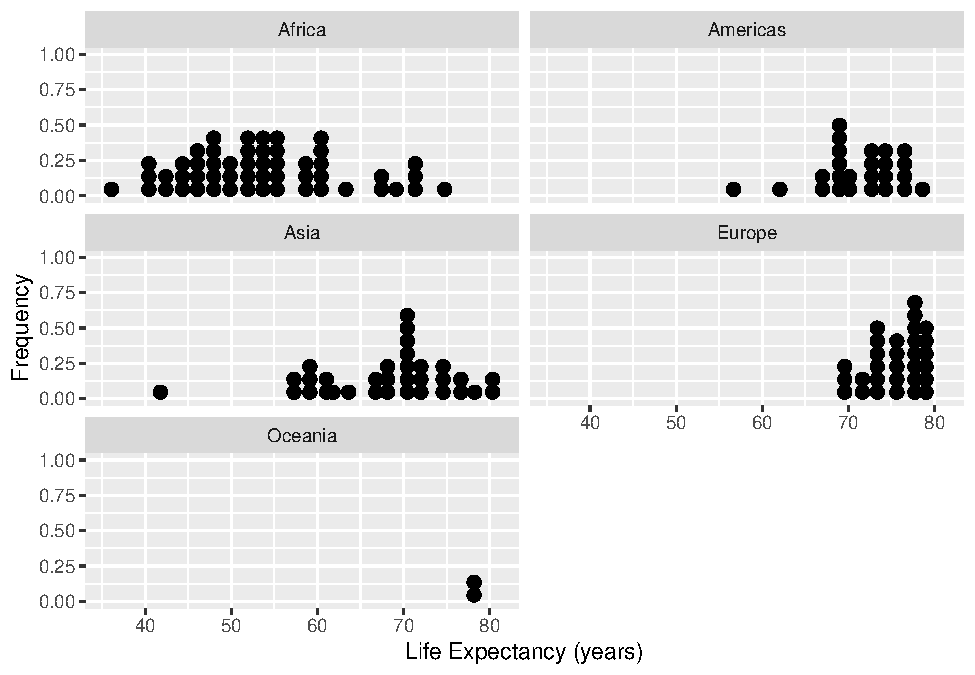
\includegraphics{bookdown-R-Essentials_files/figure-latex/unnamed-chunk-78-1.pdf}

\begin{Shaded}
\begin{Highlighting}[]
\CommentTok{#}
\KeywordTok{ggplot}\NormalTok{(}\DataTypeTok{data=}\NormalTok{ds, }\KeywordTok{aes}\NormalTok{(}\DataTypeTok{x=}\NormalTok{party)) }\OperatorTok{+}\StringTok{ }
\StringTok{  }\KeywordTok{geom_bar}\NormalTok{(}\KeywordTok{aes}\NormalTok{(}\DataTypeTok{fill=}\NormalTok{party)) }\OperatorTok{+}
\StringTok{  }\KeywordTok{facet_wrap}\NormalTok{( }\OperatorTok{~}\StringTok{ }\NormalTok{chamber) }\OperatorTok{+}
\StringTok{  }\KeywordTok{labs}\NormalTok{(}\DataTypeTok{x=}\StringTok{"Party"}\NormalTok{, }\DataTypeTok{y=}\StringTok{"Count"}\NormalTok{)}
\end{Highlighting}
\end{Shaded}

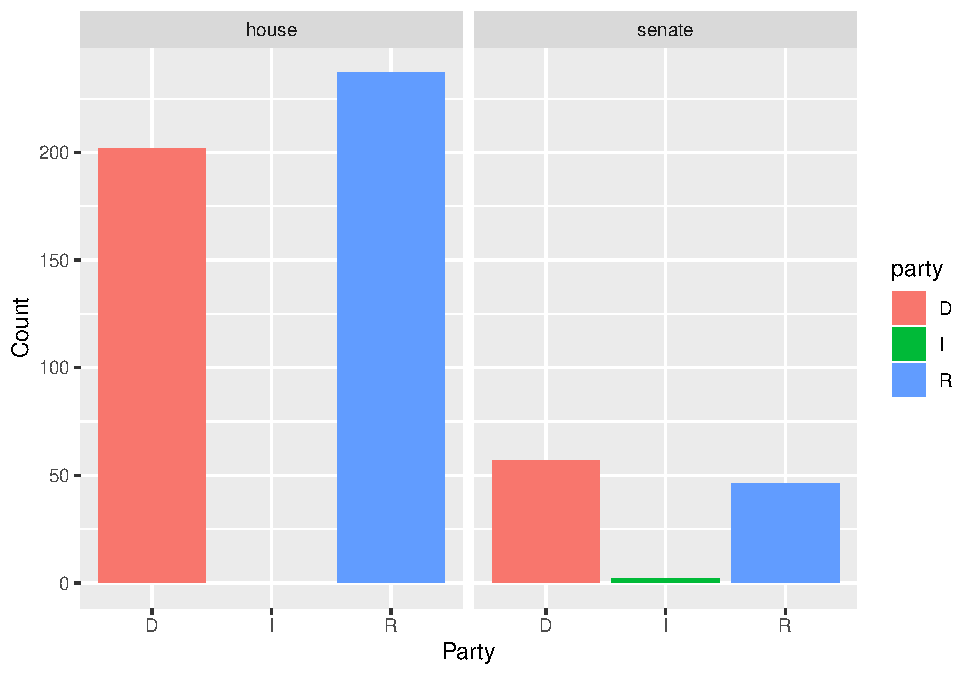
\includegraphics{bookdown-R-Essentials_files/figure-latex/unnamed-chunk-78-2.pdf}

\begin{Shaded}
\begin{Highlighting}[]
\CommentTok{#  The next display attempts to use percentages on the vertical axis defined within chamber.}
\CommentTok{# This means the next command must list chamber as the FIRST group_by variable.}
\NormalTok{ds <-}\StringTok{ }\NormalTok{ds1 }\OperatorTok\StringTok{ }\KeywordTok{group_by}\NormalTok{(chamber,party)  }\OperatorTok
\StringTok{   }\KeywordTok{summarise}\NormalTok{ (}\DataTypeTok{n =} \KeywordTok{n}\NormalTok{()) }\OperatorTok
\StringTok{  }\KeywordTok{mutate}\NormalTok{(}\DataTypeTok{pct =} \DecValTok{100}\OperatorTok{*}\NormalTok{n }\OperatorTok{/}\StringTok{ }\KeywordTok{sum}\NormalTok{(n)) }
\CommentTok{#}
\NormalTok{ds}
\end{Highlighting}
\end{Shaded}

\begin{verbatim}
## # A tibble: 5 x 4
## # Groups:   chamber [2]
##   chamber party     n   pct
##   <fct>   <fct> <int> <dbl>
## 1 house   D       202 46.0 
## 2 house   R       237 54.0 
## 3 senate  D        57 54.3 
## 4 senate  I         2  1.90
## 5 senate  R        46 43.8
\end{verbatim}

\begin{Shaded}
\begin{Highlighting}[]
\CommentTok{#}
\KeywordTok{ggplot}\NormalTok{(}\DataTypeTok{data=}\NormalTok{ds, }\KeywordTok{aes}\NormalTok{(}\DataTypeTok{x=}\NormalTok{party, }\DataTypeTok{y=}\NormalTok{pct)) }\OperatorTok{+}\StringTok{ }\KeywordTok{geom_bar}\NormalTok{(}\KeywordTok{aes}\NormalTok{(}\DataTypeTok{fill=}\NormalTok{party),}\DataTypeTok{stat=}\StringTok{"identity"}\NormalTok{) }\OperatorTok{+}
\StringTok{  }\KeywordTok{facet_wrap}\NormalTok{( }\OperatorTok{~}\StringTok{ }\NormalTok{chamber) }\OperatorTok{+}
\StringTok{  }\KeywordTok{labs}\NormalTok{(}\DataTypeTok{x=}\StringTok{"Party"}\NormalTok{, }\DataTypeTok{y=}\StringTok{"Percent"}\NormalTok{)}
\end{Highlighting}
\end{Shaded}

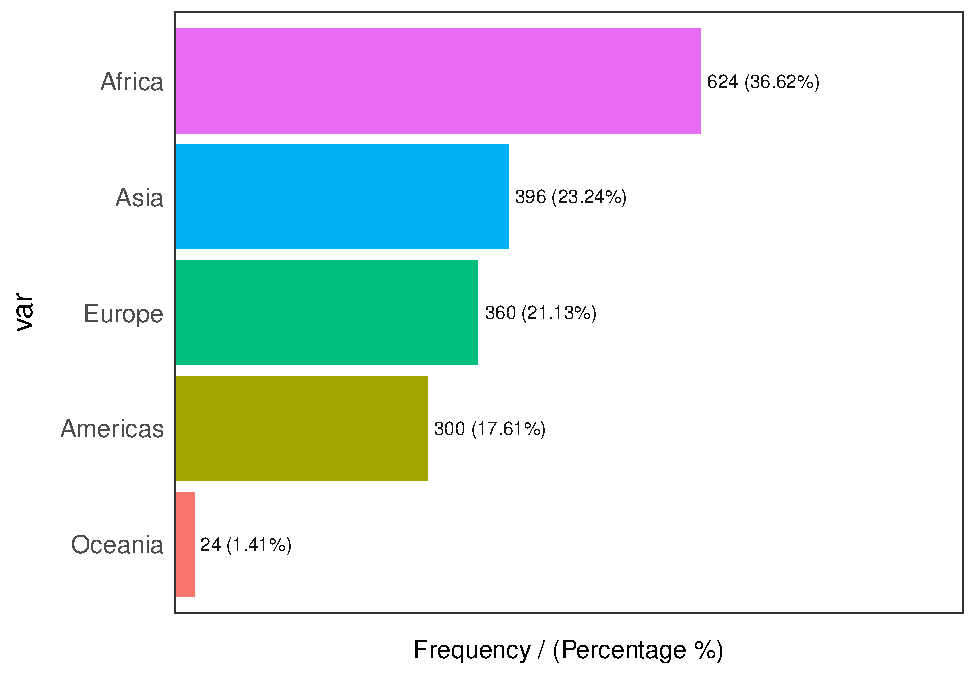
\includegraphics{bookdown-R-Essentials_files/figure-latex/unnamed-chunk-79-1.pdf}

\begin{Shaded}
\begin{Highlighting}[]
\NormalTok{ds1 <-}\StringTok{ }\NormalTok{congage }\OperatorTok\StringTok{ }\KeywordTok{filter}\NormalTok{(congress }\OperatorTok{>}\StringTok{ }\DecValTok{112}\NormalTok{) }\OperatorTok\StringTok{ }\KeywordTok{select}\NormalTok{(congress,chamber,state,party,incumbent,age) }\OperatorTok
\StringTok{ }\KeywordTok{mutate}\NormalTok{(}\DataTypeTok{party =} \KeywordTok{factor}\NormalTok{(party,}\DataTypeTok{levels=}\KeywordTok{c}\NormalTok{(}\StringTok{"D"}\NormalTok{,}\StringTok{"I"}\NormalTok{,}\StringTok{"R"}\NormalTok{)),}
                    \DataTypeTok{chamber =} \KeywordTok{factor}\NormalTok{(chamber)) }\OperatorTok\StringTok{ }
\StringTok{  }\KeywordTok{na.omit}\NormalTok{()}
\CommentTok{#}
\NormalTok{ds <-}\StringTok{ }\NormalTok{ds1 }\OperatorTok\StringTok{ }\KeywordTok{group_by}\NormalTok{(chamber,party)  }\OperatorTok
\StringTok{   }\KeywordTok{summarise}\NormalTok{ (}\DataTypeTok{n =} \KeywordTok{n}\NormalTok{()) }\OperatorTok
\StringTok{  }\KeywordTok{mutate}\NormalTok{(}\DataTypeTok{pct =} \DecValTok{100}\OperatorTok{*}\NormalTok{n }\OperatorTok{/}\StringTok{ }\KeywordTok{sum}\NormalTok{(n)) }
\CommentTok{#}
\KeywordTok{ggplot}\NormalTok{(}\DataTypeTok{data=}\NormalTok{ds, }\DataTypeTok{mapping=}\KeywordTok{aes}\NormalTok{(}\DataTypeTok{x=}\NormalTok{chamber,}\DataTypeTok{y=}\NormalTok{pct,}\DataTypeTok{fill=}\NormalTok{party)) }\OperatorTok{+}\StringTok{ }
\StringTok{  }\KeywordTok{geom_col}\NormalTok{() }\OperatorTok{+}
\StringTok{  }\KeywordTok{labs}\NormalTok{(}\DataTypeTok{x=}\StringTok{"Chamber"}\NormalTok{, }\DataTypeTok{y=}\StringTok{"Percent"}\NormalTok{)}
\end{Highlighting}
\end{Shaded}

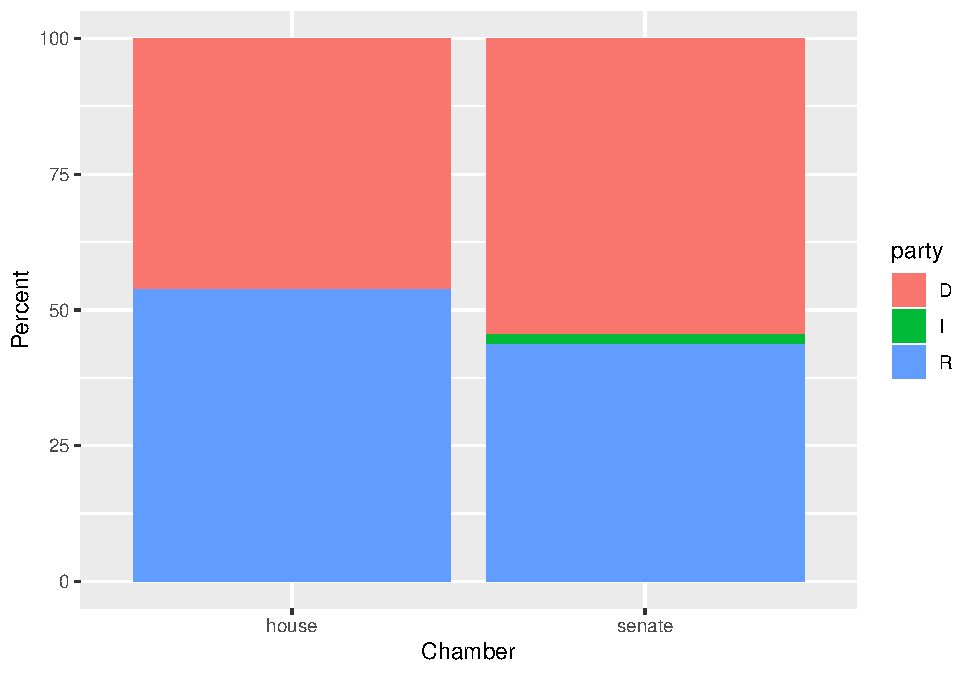
\includegraphics{bookdown-R-Essentials_files/figure-latex/unnamed-chunk-80-1.pdf}

\begin{Shaded}
\begin{Highlighting}[]
\NormalTok{ds1 <-}\StringTok{ }\NormalTok{congage }\OperatorTok\StringTok{ }\KeywordTok{filter}\NormalTok{(congress }\OperatorTok{>}\StringTok{ }\DecValTok{112}\NormalTok{) }\OperatorTok\StringTok{ }\KeywordTok{select}\NormalTok{(congress,chamber,state,party,incumbent,age) }\OperatorTok
\StringTok{ }\KeywordTok{mutate}\NormalTok{(}\DataTypeTok{party =} \KeywordTok{factor}\NormalTok{(party,}\DataTypeTok{levels=}\KeywordTok{c}\NormalTok{(}\StringTok{"D"}\NormalTok{,}\StringTok{"I"}\NormalTok{,}\StringTok{"R"}\NormalTok{)),}
                    \DataTypeTok{chamber =} \KeywordTok{factor}\NormalTok{(chamber)) }\OperatorTok\StringTok{ }
\StringTok{  }\KeywordTok{na.omit}\NormalTok{()}
\CommentTok{#}
\NormalTok{ds1 }\OperatorTok\StringTok{ }\KeywordTok{group_by}\NormalTok{(chamber,party)  }\OperatorTok
\StringTok{   }\KeywordTok{summarise}\NormalTok{ (}\DataTypeTok{n =} \KeywordTok{n}\NormalTok{()) }\OperatorTok
\StringTok{  }\KeywordTok{mutate}\NormalTok{(}\DataTypeTok{pct =} \DecValTok{100}\OperatorTok{*}\NormalTok{n }\OperatorTok{/}\StringTok{ }\KeywordTok{sum}\NormalTok{(n)) }\OperatorTok
\KeywordTok{ggplot}\NormalTok{( }\DataTypeTok{mapping=}\KeywordTok{aes}\NormalTok{(}\DataTypeTok{x=}\NormalTok{chamber,}\DataTypeTok{y=}\NormalTok{pct,}\DataTypeTok{fill=}\NormalTok{party)) }\OperatorTok{+}\StringTok{ }
\StringTok{  }\KeywordTok{geom_col}\NormalTok{() }\OperatorTok{+}
\StringTok{  }\KeywordTok{coord_flip}\NormalTok{() }\OperatorTok{+}
\StringTok{  }\KeywordTok{labs}\NormalTok{(}\DataTypeTok{x=}\StringTok{"Chamber"}\NormalTok{, }\DataTypeTok{y=}\StringTok{"Percent"}\NormalTok{)}
\end{Highlighting}
\end{Shaded}

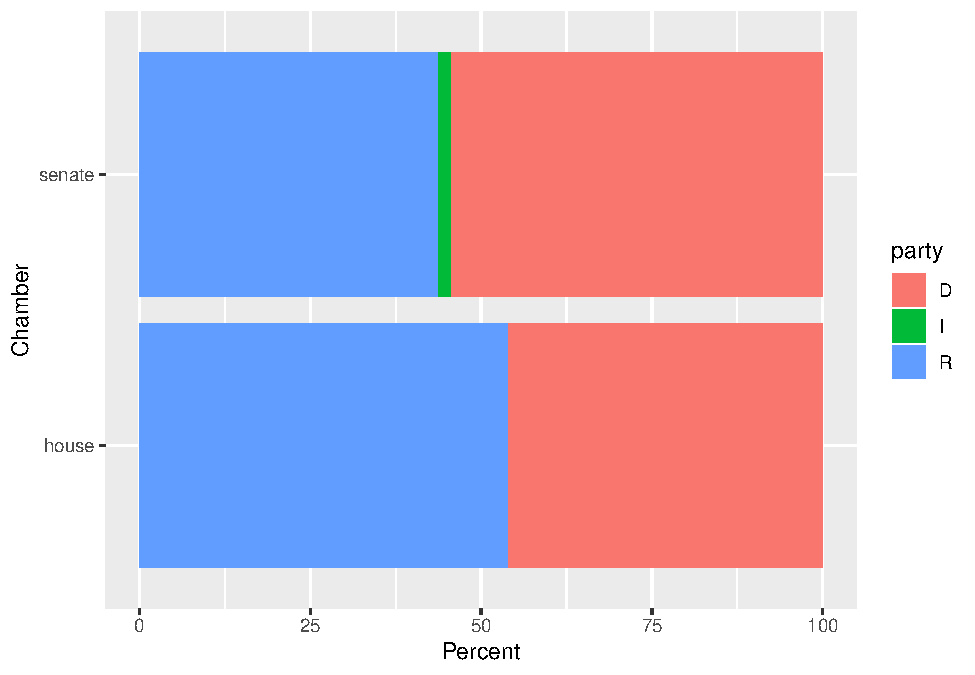
\includegraphics{bookdown-R-Essentials_files/figure-latex/unnamed-chunk-81-1.pdf}

\bibliography{book.bib,packages.bib}

\end{document}
